\documentclass[12pt,a4paper]{ctexart}
\usepackage{geometry}
\geometry{left=3.17cm,right=3.17cm,top=2.54cm,bottom=2.54cm}
\usepackage{graphicx}
\usepackage{booktabs}
\usepackage{float}
\usepackage{subcaption}
\usepackage{amsmath,amssymb}
\usepackage{multirow}
\usepackage{longtable}
\usepackage{hyperref}
\hypersetup{colorlinks=true,linkcolor=black,citecolor=black,urlcolor=black}
\usepackage{titletoc}
\usepackage[dvipsnames,svgnames,x11names]{xcolor}
\usepackage{threeparttable}
\usepackage{setspace}
\usepackage{appendix}
\usepackage{array}
\usepackage{tabularx}
\usepackage{ragged2e}
\usepackage{indentfirst}
\usepackage{fancyhdr}
\xeCJKsetup{AutoFakeBold=true}
\setCJKfamilyfont{zhsong}[AutoFakeBold=5.0]{STSong}

\usepackage{caption}
\DeclareCaptionLabelSeparator{twospaces}{\hspace{1em}} % 图/表序号与名称间两空格
\captionsetup{
  labelsep=twospaces,
  justification=centering,
  singlelinecheck=false
}
\captionsetup[table]{position=top, name=表}
\captionsetup[figure]{position=bottom, name=图}
\captionsetup[figure]{position=bottom, name=图}

\usepackage{colortbl}
\usepackage{dashrule}
\usepackage{etoolbox}
\AtBeginEnvironment{tabular}{\singlespacing}

\setlength{\parindent}{2em}
\setlength{\parskip}{0pt}
% 固定行距24磅（正文与标题统一）
\AtBeginDocument{\fontsize{12pt}{24bp}\selectfont\setlength{\parindent}{2\ccwd}}

% ─── 页码页眉样式设置──────────────────────────────
\pagestyle{fancy}
\fancyhf{} % 清除默认的页眉页脚设置

\renewcommand{\headrulewidth}{0pt} % 去掉页眉那条横线
\fancyhead[L]{\zihao{-5}\kaishu\textcolor{gray} \leftmark}
\fancyfoot[C]{\zihao{5}\textcolor{gray}{\thepage}} % 核心修改：页脚中央灰色页码

\ctexset{
section={
  format=\heiti\fontsize{15pt}{24pt}\selectfont\raggedright,
  name={,、},
  number=\chinese{section},
  beforeskip=0pt,
  afterskip=0pt
},
subsection={
  format=\kaishu\fontsize{14pt}{24pt}\selectfont\raggedright,
  name={（,）},
  number=\chinese{subsection},
  beforeskip=0pt,
  afterskip=0pt
},
subsubsection={
  format=\songti\bfseries\fontsize{12pt}{24pt}\selectfont\raggedright,
  name={,\hspace{0.5em}},
  number=\arabic{subsubsection}.,
  beforeskip=0pt,
  afterskip=0pt
}
}

% ─── 目录样式 ──────────────────────────────────────────────
\titlecontents{section}[0em]
  {\addvspace{4pt}\songti\bfseries} % 宋体加粗
  {\contentslabel{1.8em}}{}
  {\titlerule*[0.5pc]{.}\contentspage}
\titlecontents{subsection}[2em]
  {\addvspace{1pt}\songti}         % 宋体
  {\contentslabel{2.4em}}{}
  {\titlerule*[0.5pc]{.}\contentspage}
\titlecontents{subsubsection}[4.6em]
  {\songti}                        % 宋体
  {\contentslabel{3em}}{}
  {\titlerule*[0.5pc]{.}\contentspage}

% ─── 关键词命令 ────────────────────────────────────────────
\newcommand{\keywords}[1]{%
  \vspace{0.9em}%
  \noindent{\bfseries 关键词：}#1\par%
}

\begin{document}


% ════════════════════════════════════════════
% ②  摘要 + 关键词
% ════════════════════════════════════════════
\clearpage
\thispagestyle{empty}
\vspace*{0.6cm}
\begin{center}
    {\songti\zihao{3} \textbf{中国碳达峰路径的驱动机制识别与多情景预测}}
\end{center}
\vspace{1.5em}
\begin{center}
{\centering\heiti\zihao{4} 摘要\par}
\end{center}
\vspace{0.6em}

\setlength{\parindent}{2em}
本文聚焦我国碳达峰目标实现过程中的关键驱动机制与未来路径预测问题，基于2005—2022年国家级观测数据与2023—2024年外推衔接数据，构建融合扩展STIRPAT、EKC检验、中介效应分析、多模型滚动预测与多情景模拟的综合分析框架。实证结果显示，受小样本自由度约束，扩展STIRPAT估计中仅煤炭占比在95\%置信水平下保持显著正向影响（弹性约3.3791）；人均GDP、能源强度等变量虽点估计多为正，但置信区间较宽且包含零。滚动一步预测比较表明，AR2 模型外推表现最稳健（RMSE=1323.36，MAPE=3.32\%）；而引入高维特征的多变量回归与复杂机器学习模型（XGBoost、随机森林）因样本量极小导致严重过拟合，误差急剧放大。多情景模拟显示，到2035年基准、低碳和深度脱碳情景下碳排放分别约为39127.33\,Mt、33013.06\,Mt和27766.48\,Mt。研究为国家层面优化减排路径、协同推进能源替代与产业升级提供量化依据。

\keywords{碳达峰；STIRPAT模型；EKC假说；滚动预测；情景模拟}

% ════════════════════════════════════════════
% ③  目录
% ════════════════════════════════════════════
\clearpage
\thispagestyle{empty}
{\centering\heiti\zihao{4} 目录\par}
\vspace{0.5em}
\begingroup
\renewcommand{\contentsname}{}
\tableofcontents
\endgroup
\clearpage

% ════════════════════════════════════════════
% ④  表格与插图清单
% ════════════════════════════════════════════
\clearpage
\thispagestyle{empty}
{\centering\heiti\zihao{4} 表格与插图清单\par}
\vspace{1em}

\noindent{\songti\bfseries 表格目录}\par
\vspace{0.5em}
\noindent 表1\quad 扩展STIRPAT模型变量说明 \dotfill \pageref{tab:stirpat_vars}\par
\noindent 表2\quad 扩展STIRPAT主要弹性系数估计结果 \dotfill \pageref{tab:stirpat_coeff}\par
\noindent 表3\quad 主要模型预测误差比较 \dotfill \pageref{tab:model_perf}\par
\noindent 表4\quad 多情景核心参数设定表 \dotfill \pageref{tab:scenario_params}\par
\noindent 表5\quad 2035年不同情景碳排放预测结果 \dotfill \pageref{tab:scenario_2035}\par
\noindent 表6\quad 样本描述性统计 \dotfill 附录\par

\vspace{1.2em}
\noindent{\songti\bfseries 插图目录}\par
\vspace{0.5em}
\noindent 图1\quad 2005—2024年中国碳排放总量变化趋势 \dotfill \pageref{fig:co2_trend}\par
\noindent 图2\quad 2005—2024年GDP与碳排放双轴对比 \dotfill \pageref{fig:gdp_co2}\par
\noindent 图3\quad 核心变量相关性矩阵热力图 \dotfill \pageref{fig:corr}\par
\noindent 图4\quad 产业结构演化趋势图 \dotfill \pageref{fig:industry_structure}\par
\noindent 图5\quad 能源总量与煤炭依赖三维联动图 \dotfill \pageref{fig:energy_structure}\par
\noindent 图6\quad 城镇化率变化趋势 \dotfill \pageref{fig:urbanization_rate}\par
\noindent 图7\quad EKC检验：人均GDP与碳排放关系 \dotfill \pageref{fig:ekc}\par
\noindent 图8\quad 中介效应路径示意图 \dotfill \pageref{fig:mediation}\par
\noindent 图9\quad 扩展STIRPAT关键弹性系数图 \dotfill \pageref{fig:stirpat}\par
\noindent 图10\quad 技术创新能力三维轨迹图 \dotfill \pageref{fig:innovation_3d}\par
\noindent 图11\quad 多模型滚动预测误差比较 \dotfill \pageref{fig:model_perf}\par
\noindent 图12\quad 基于XGBoost模型的特征重要性SHAP分析 \dotfill \pageref{fig:shap}\par
\noindent 图13\quad 不同情景下碳排放路径预测比较（2025—2035） \dotfill \pageref{fig:scenario_paths}\par
\noindent 图14\quad 不同情景峰值年份与峰值规模三维比较 \dotfill \pageref{fig:peak_3d}\par
\noindent 图15\quad 实际值与预测值对比图 \dotfill 附录\par
\noindent 图16\quad 集成模型残差诊断图 \dotfill 附录\par
\noindent 图17\quad 碳排放与GDP增速对比图 \dotfill 附录\par
\noindent 图18\quad GDP、城镇化与碳排放三维响应图 \dotfill 附录\par
\noindent 图19\quad 能源与结构特征雷达图 \dotfill 附录\par
\noindent 图20\quad 2035年情景差异瀑布分解图 \dotfill 附录\par
\noindent 图21\quad 滚动相关热力图 \dotfill 附录\par
\clearpage


% 正文页码从第1页重新编列
\setcounter{page}{1}
\pagenumbering{arabic}

% 正文总标题（方正小标宋简体三号，居中）
\begin{center}
{\zihao{3}\CJKfamily{zhsong}\bfseries 中国碳达峰路径的驱动机制识别与多情景预测}
\end{center}
\vspace{0.5em}

\section{引言}
\subsection{研究背景}
在全球“双碳”战略背景下，科学识别碳排放驱动因素并预测达峰路径是核心议题。碳排放受经济规模、产业结构、能源与技术等多因素交织影响。在“双碳”目标下，理清这些因素的联动机制并预测达峰路径，是当前亟待解决的现实问题。

从研究尺度看，省级面板分析能够呈现区域差异，但在小样本宏观时序数据与统计口径一致性约束下，往往面临变量定义不统一、口径协调成本高、结果解释分散等问题。与之相比，国家级时间序列分析可以在较低的数据整合成本下形成统一口径，更适合回答总量控制、达峰时点和政策路径等宏观问题。在面向公共政策评估的研究语境中，国家级框架更便于形成“数据清洗—机制识别—预测比较—情景模拟—政策解释”的完整链条，并在有限数据可得性条件下保持结论可复核性。

\subsection{研究问题与研究意义}
围绕国家层面碳达峰路径识别，本文聚焦三个递进问题：第一，人口、富裕度、能源强度、能源结构、产业结构、技术进步和治理投入等变量对碳排放的方向与强度如何；第二，在国家级小样本时间序列条件下，不同预测模型的外推能力是否存在稳定差异；第三，在不同政策强度下，未来碳排放峰值水平与达峰路径将出现何种分化。上述问题分别对应“机制解释”“预测适配”“政策模拟”三个层次，构成本文的主线。

从现实层面看，国家级碳达峰预测有助于评估减排路径的可行性，并为能源结构优化、产业升级、技术创新与环境治理政策提供量化证据。相比只给出总量趋势，机制识别能够进一步回答“为什么会出现该趋势”，从而提高政策建议的针对性。对当前“双碳”政策实践而言，准确识别煤炭依赖、工业结构、技术扩散和治理投入在排放变化中的相对作用，是优化政策组合的重要前提。

从方法层面看，将解释性模型与预测性模型结合，可以避免“只解释不预测”或“只预测不解释”的单一化研究倾向。扩展STIRPAT和EKC检验强调变量作用机制，中介分析强调结构传导路径，滚动一步预测强调真实外推能力，多情景模拟强调政策含义外化。多方法协同不仅提升研究严谨性，也增强了结果在公共政策评估语境中的可检验性和可沟通性。

\subsection{研究思路、创新点与边界}
本文研究思路可概括为“数据整合—机制识别—预测比较—情景模拟—政策解释”五个环节。首先，基于CEADs省级表观碳排放清单按年汇总构建国家级碳排放序列，并与国家统计局宏观指标进行口径匹配；其次，通过EKC检验和扩展STIRPAT模型识别核心驱动因素及其弹性方向；再次，利用中介框架讨论能源结构、技术进步和产业结构之间的作用链；随后，在滚动一步预测框架下比较多种模型的外推表现；最后，设定基准、低碳和深度脱碳三类情景并开展峰值路径模拟，形成政策含义。

本文创新主要体现在四个方面。第一，构建了“机制解释—预测比较—情景模拟”一体化的分析框架，实现了从现象解释到政策推演的连贯分析。第二，在国家级时序框架内，将能源结构、产业结构、技术进步与治理投入纳入统一分析体系，提升变量覆盖的现实对应性。第三，采用滚动一步预测评估模型而非仅比较样本内拟合，强化了对外推能力的识别。第四，结合滚动预测误差与情景偏离度，构建了政策效果的动态监测思路，为后续减排参数的年度调整提供量化参考。

需要说明的是，本文结论适用于国家总量层面，不直接推断区域异质性和行业细分机制；2023—2024年数据用于预测衔接与情景延展，不参与机制回归估计。该边界设置有助于保证统计推断的口径一致性，避免将预测值误作观测事实。

\section{文献综述}
\subsection{碳排放驱动因素研究}
现有研究关于碳排放驱动机制的讨论，主要沿着“恒等式分解—计量回归—系统协同”三条路径展开。第一类研究以Kaya恒等式和LMDI分解为代表，强调将碳排放变化拆解为人口、经济、能源效率和能源结构等可解释分量，优点是结构清晰、政策可读性强，适合做事后归因。第二类研究以STIRPAT扩展模型为代表，将IPAT关系随机化并引入弹性参数，使变量作用可在统计框架下估计，更适合考察多因素同时作用时的边际效应方向和强度。

近年来，驱动因素研究逐步从单一变量解释走向多机制协同识别。大量研究指出，煤炭依赖和高耗能产业比重通常与排放增长同向；而产业升级、能源替代、技术进步和治理投入在中长期具有减排潜力。值得关注的是，不同变量之间并非独立作用，例如能源结构变化往往伴随技术改造和产业调整，这使“单因素—单结论”的分析框架难以完整解释排放路径。因而，能够同时覆盖规模效应、结构效应和技术效应的综合识别框架，正在成为主流方向。

\subsection{碳排放预测方法研究}
碳排放预测方法已从传统统计模型扩展到机器学习和集成学习。传统时间序列模型（如AR类、趋势外推）在小样本、低频数据场景下通常更稳定，参数解释也较直接；但面对复杂非线性关系时，其刻画能力受到限制。机器学习模型在高维特征关系捕捉方面具备优势，尤其在样本容量较大时能体现更高拟合能力，不过其外推稳定性和可解释性在小样本条件下常受质疑。

为兼顾准确性与稳健性，越来越多研究采用多模型比较或模型集成策略。该思路不预设“复杂模型必然最优”，而是在统一评价指标下比较不同模型在外推任务中的表现，再据此选择适配模型。与此同时，SHAP等可解释方法被用于连接“黑箱预测”与“机制解释”，使预测模型在给出结果的同时能够提供变量重要性证据。总体来看，预测研究的发展趋势并非单纯追求复杂度，而是强调模型结构与数据规模、研究目标和解释需求之间的匹配。

\subsection{情景模拟与政策评估研究}
在达峰与减排研究中，情景模拟常用于评估政策强度变化对未来路径的影响。已有研究普遍构建基准情景与强化减排情景，通过设定能源结构、产业结构和技术进步等关键参数，比较不同路径下的峰值时点与峰值规模。该类方法的优势在于可将抽象政策目标转化为可量化路径，从而增强政策讨论的可操作性。

但现有情景研究也存在两个共性问题：一是部分参数设定与机制估计脱节，导致情景设计缺乏统计支撑；二是部分研究只给出终点数值，缺少对路径斜率、峰后下降速度和政策成本含义的解释。由此，情景模拟不仅需要“给出不同结果”，更需要解释“为什么出现差异、差异来自哪些变量变化”。这要求机制分析与情景分析在同一框架内衔接，而非各自独立。

\subsection{现有研究不足与本文定位}
综合已有文献，可以归纳出三点不足。其一，“机制解释”与“预测精度”常被分离处理，导致研究结论停留在解释层面或预测层面。其二，部分研究仍以样本内拟合表现评价预测能力，难以反映真实外推场景下的模型稳定性。其三，情景分析与机制识别衔接不足，政策建议容易停留于原则性表述，缺少与实证结果一一对应的证据链。

基于此，本文在国家级时间序列数据基础上，构建集扩展STIRPAT、EKC检验、中介路径分析、滚动一步预测比较与多情景模拟于一体的综合框架，力图实现三方面改进：第一，在同一数据口径下同时回答“为什么变化”和“如何变化”；第二，以滚动外推误差而非样本内拟合作为预测比较标准；第三，将机制证据嵌入情景路径解释，提升政策讨论的实证支撑力度。该定位使本文既保持统计解释的严谨性，也具备面向政策应用的可读性与可操作性。

\section{数据说明与变量设计}
\subsection{数据来源与口径统一}
本文数据主要来自CEADs省级表观碳排放清单与国家统计局年度数据库，并辅以生态环境经济核算报告和公开统计资料进行口径核对。由于碳排放原始数据按省份发布，本文先按年份进行全国汇总，构建国家级碳排放总量序列；宏观解释变量则直接采用国家级年度指标，以保证时间序列的一致性和可比性。

数据源于 CEADs 省级清单与国家统计局数据库，辅以生态环境经济核算报告进行核对。因变量$C_t$来源于 CEADs 碳排放清单。该清单包含化石燃料燃烧和过程排放等信息，本文在同一年份内对省级排放值求和，得到国家总量。解释变量包括人口、GDP、人均GDP、城镇化率、第二产业占比、能源消费总量、煤炭消费占比、创新与治理代理指标等。通过该组合，本文从人口、经济、结构、能源、技术和治理六个维度描述碳排放驱动机制。

在国家级研究框架下，口径统一比变量数量更重要。为此本文遵循三项原则：第一，同一变量仅保留一个统计口径，避免不同来源混用；第二，优先采用连续年份完整、可追溯的数据源；第三，必要时对单位进行统一换算并在模型前进行一致性检查。该处理有助于降低“口径漂移”造成的估计偏差。

\subsection{变量构造与指标定义}
设$t$为年份，$C_t$为全国碳排放总量，$P_t$为总人口，$A_t$为富裕度，核心变量定义如下：
\begin{align}
C_t &= \sum_{i=1}^{N} C_{it}, \\
A_t &= \frac{GDP_t}{P_t}, \\
EI_t &= \frac{EC_t}{GDP_t}, \\
CI_t &= \frac{C_t}{GDP_t}, \\
PC_t &= \frac{C_t}{P_t}.
\end{align}

其中，$EC_t$为能源消费总量，$EI_t$表示能源强度，$CI_t$为碳强度，$PC_t$为人均碳排放。能源结构变量以煤炭消费占比表示，记为$CS_t$；城镇化变量以城镇人口占比表示，记为$UR_t$；产业结构变量以第二产业增加值占比表示，记为$IS_t$；技术进步变量以有效发明专利和科研机构规模的组合代理表示，记为$TP_t$；环境治理变量以污染治理投资强度表示。

本文在变量选取上注重理论与数据的匹配，所选指标均可从公开统计口径获取，且保证了跨年份的量纲一致，以增强实证结果的可靠性。相较于引入大量高维指标，本文更强调核心变量的稳定测度，以保证小样本时序估计的有效性。

\subsection{变量预处理与统计策略}
为了提高估计稳定性，本文对规模变量（如人口、富裕度、能源强度）采用对数变换，使系数可解释为弹性并缓解异方差。比例变量（如煤炭占比、城镇化率、产业结构占比）保留原始比例形式，以便直接解释结构变化的边际影响。对于数量级差异显著的变量，在进入机器学习模型前进行标准化处理，用于提升训练稳定性。

在统计分析流程上，本文先进行描述统计与相关性检验，再进入机制回归与预测比较，最后进行情景模拟。该顺序可确保每一步结论都建立在前一环节的可验证结果之上，避免直接从模型输出跳到政策结论。

\subsection{描述性统计特征}
描述性统计结果表明，在2005—2022年观测区间内，我国碳排放总量均值约30566.50 Mt，最小值17516.39 Mt，最大值40358.26 Mt，呈现显著长期上行特征。同期GDP均值约654617.21亿元，人均GDP均值约4.73万元，城镇化率均值约54.90\%，第二产业占比均值约42.24\%，能源消费总量均值约417734.00万吨标准煤，煤炭占比均值约64.72\%。

这些统计特征共同说明：一方面，经济扩张和能源总量增长仍是排放上行的重要背景；另一方面，产业和能源结构已出现持续调整，为后续达峰路径优化提供了可能。技术创新代理变量在样本期内显著增长，提示创新要素积累正在形成中长期减排潜力，但其效应释放存在时滞。

\subsection{缺失值处理与样本边界}
本文保持2005—2024年研究时段不变。根据数据可得性，碳排放观测值覆盖2005—2022年，2023—2024年仅在预测与情景模拟中用于趋势衔接，不纳入机制回归和描述统计的观测样本。也即，实证估计基于真实观测区间，预测值只用于外推比较与路径展示。

该处理的意义在于：既保证图表与情景分析的时间连续性，又避免将模型推断误作事实数据。为强化边界清晰性，本文在相关章节始终区分“观测值”“预测值”和“情景值”三类数据，并在解释结论时仅对观测样本作统计推断。

\subsection{数据质量控制与稳健性说明}
为降低测度误差风险，本文进行了跨来源口径核对、异常年份回查以及结果一致性核验三类质量控制，如遇数据冲突，则重新核对原始来源并调整模型设定。

需要指出，本文并不以“覆盖全部可能变量”为目标，而是以“核心机制可被稳定识别”为优先原则。这一取舍有助于在有限数据可得性条件下保证结论可靠性，并为后续研究在更长样本和更细粒度数据基础上的扩展留出空间。

\section{模型构建}
\subsection{建模目标与总体框架}
本文的建模目标包含两个互补维度：一是解释维度，即识别碳排放变化的主要驱动机制与作用方向；二是预测维度，即在真实外推场景下比较不同模型的稳定性，并据此开展政策情景模拟。围绕该目标，本文采用“EKC检验 + 扩展STIRPAT + 中介分析 + 滚动预测 + 情景模拟”的组合框架，以保证机制识别与路径预测在同一口径下衔接。

该框架的逻辑顺序为：先通过EKC检验判断经济发展与排放关系是否存在阶段性，再利用扩展STIRPAT估计多因素边际影响，随后用中介框架讨论能源结构影响的传导渠道；在解释基础上，再以滚动一步预测比较模型适配性，最后通过情景设定将统计结果转化为可比较的政策路径。

\subsection{环境库兹涅茨曲线检验}
为检验经济增长与碳排放之间的非线性关系，本文构建对数双次项EKC模型：
\begin{equation}
\ln C_t = \alpha_0 + \alpha_1 \ln A_t + \alpha_2 (\ln A_t)^2 + \varepsilon_t,
\end{equation}
其中$C_t$为第$t$年全国碳排放总量（Mt），$A_t$为人均GDP（万元），$\varepsilon_t$为随机误差项。对两侧变量取对数后，$\alpha_1$可解释为人均GDP对碳排放的弹性，$\alpha_2$捕捉该弹性随收入水平的变化方向。

EKC假说的理论内涵可由排放对人均收入的条件边际效应刻画：
\begin{equation}
\frac{\partial \ln C_t}{\partial \ln A_t} = \alpha_1 + 2\alpha_2 \ln A_t.
\end{equation}
当$\alpha_1>0$且$\alpha_2<0$时，上式随收入增长单调递减，意味着存在排放强度”脱钩拐点”，对应人均GDP的峰值点为：
\begin{equation}
A^* = \exp\!\left(-\frac{\alpha_1}{2\alpha_2}\right).
\end{equation}
若$A^*$落在样本范围内，则支持样本期内存在倒U型关系；若两系数同号或$A^*$远超样本上限，则说明当前阶段排放与收入仍呈单调关系。

EKC检验在本文中的作用并非单独给出因果结论，而是判断”经济规模扩张是否已出现边际减排拐点迹象”，为后续机制解释提供阶段性背景。该定位可避免将简单二次拟合过度解读为结构性因果关系。

{\songti\bfseries{}注：受限于样本长度与对数变换后的极值平滑效应，图7采用水平值二次多项式进行可视化趋势拟合，以更直观地展示拐点形态；公式(6)的对数形式用于理论机制说明与弹性计算基准。}

\subsection{扩展STIRPAT模型}
经典IPAT恒等式将环境压力$I$表达为人口$P$、富裕度$A$与技术水平$T$的乘积：
\begin{equation}
I = P \cdot A \cdot T.
\end{equation}
STIRPAT（Stochastic Impacts by Regression on Population, Affluence and Technology）对其进行随机化扩展：
\begin{equation}
I = a P^b A^c T^d \cdot e,
\end{equation}
其中$a$为模型系数，$b,c,d$为各因素的弹性参数，$e$为随机误差。对两侧取自然对数，得到可估计的对数线性形式：
\begin{equation}
\ln I_t = \ln a + b\ln P_t + c\ln A_t + d\ln T_t + \ln e_t.
\end{equation}
此时$b,c,d$分别表示人口、富裕度和技术对环境压力的弹性，便于直接比较各驱动因素的相对贡献。

结合我国碳排放的现实机制，本文在标准三因素框架基础上引入能源结构、城镇化和产业结构，扩展为六因素模型：
\begin{equation}
\ln C_t = \beta_0 + \beta_1 \ln A_t + \beta_2 \ln EI_t + \beta_3 CS_t + \beta_4 UR_t + \beta_5 TP_t + \beta_6 IS_t + \varepsilon_t,
\end{equation}
各变量含义及预期符号如表~\ref{tab:stirpat_vars}所示。

\begin{table}[H]
\centering
\caption{扩展STIRPAT模型变量说明}
\label{tab:stirpat_vars}
\begin{tabular}{cccc}
\toprule
符号 & 含义 & 单位/度量 & 预期符号 \\
\midrule
$C_t$  & 全国碳排放总量    & Mt         & —（因变量）\\
$A_t$  & 人均GDP（富裕度） & 万元/人    & $+$ \\
$EI_t$ & 能源强度          & 万吨标煤/亿元 & $+$ \\
$CS_t$ & 煤炭消费占比      & 比例        & $+$ \\
$UR_t$ & 城镇化率          & 比例        & $\pm$ \\
$TP_t$ & 技术进步代理（有效发明专利对数） & — & $-$ \\
$IS_t$ & 第二产业增加值占比 & 比例       & $+$ \\
\bottomrule
\end{tabular}
{\footnotesize 注：技术进步预期符号为负，代表其具备减排潜力，但在小样本阶段可能受能源反弹效应干扰表现不显著。}
\end{table}

参数$\beta_1,\beta_2$的估计值可解释为弹性：例如$\hat\beta_1=0.59$表示人均GDP每增长1\%，碳排放平均增长0.59\%。$\beta_3$至$\beta_6$对应水平变量，其系数反映该变量每变动一单位时碳排放对数的变化量（半弹性）。

模型采用普通最小二乘法（OLS）估计，置信区间基于残差方差和$(X^\top X)^{-1}$矩阵的对角元素构造：
\begin{equation}
\hat\beta_j \pm z_{0.975}\cdot\hat{\sigma}\sqrt{[(X^\top X)^{-1}]_{jj}},
\end{equation}
其中$\hat\sigma^2 = \frac{\mathbf{e}^\top\mathbf{e}}{n-k}$，$n=18$为观测数，$k=7$为参数个数（含截距），自由度$n-k=11$。

该设定具有三点优势：第一，避免将人口规模与人均GDP同时引入导致的恒等式相关性干扰，降低多重共线性风险；第二，弹性系数便于比较不同变量的相对作用强度；第三，与政策变量具有直接映射，便于后续情景参数解释。

\subsection{中介效应分析}
中介效应分析用于检验自变量$X$对因变量$Y$的影响是否通过中间变量$M$部分或完全传导。本文以煤炭占比（$CS_t$）作为核心自变量$X_t$，技术进步（$TP_t$）作为潜在中介变量$M_t$，碳排放（$C_t$）的对数作为因变量$Y_t$，依次估计以下三个方程：

{\songti\bfseries{}第一步：}检验$X$对中介变量$M$的影响（$a$路径）：
\begin{equation}
M_t = \gamma_0 + \gamma_1 X_t + u_t.
\end{equation}
$\gamma_1$显著则说明能源结构对技术进步存在可识别关联。

{\songti\bfseries{}第二步：}检验$X$对$Y$的总效应（$c$路径）：
\begin{equation}
Y_t = \delta_0 + \delta_1 X_t + v_t.
\end{equation}
$\delta_1$为自变量对因变量的总效应系数。

{\songti\bfseries{}第三步：}在控制中介变量后，同时估计$X$对$Y$的直接效应（$c'$路径）与$M$对$Y$的效应（$b$路径）：
\begin{equation}
Y_t = \theta_0 + \theta_1 X_t + \theta_2 M_t + w_t.
\end{equation}

中介效应的分解关系为：
\begin{equation}
\underbrace{\delta_1}_{\text{总效应}} = \underbrace{\theta_1}_{\text{直接效应}} + \underbrace{\gamma_1 \cdot \theta_2}_{\text{间接效应（中介）}}.
\end{equation}
若$\gamma_1$与$\theta_2$均显著，且$|\theta_1| < |\delta_1|$，则可认为$M$在$X\to Y$路径上存在部分中介作用；若$\theta_1$不再显著而$\gamma_1\cdot\theta_2$显著，则为完全中介。

需要强调，中介框架在本文中用于揭示”作用链可能性”而非严格因果识别。受限于样本长度，本文更重视路径方向的一致性和经济含义的可解释性。

\subsection{滚动预测模型设计与评估}
为贴近真实应用场景，本文采用滚动一步向前预测（rolling one-step-ahead forecast）而非全样本内拟合。设共有$T$期观测，在预测第$t$期时，仅使用$\{1,2,\ldots,t-1\}$期数据估计模型参数，再预测$\hat{C}_t$，随后将窗口向前滚动一期。该策略严格避免未来信息泄露，所得误差指标更能反映模型的真实外推能力。

本文比较七类模型，各模型的数学形式与参数含义如下：

\begin{enumerate}

\item {\songti\bfseries{}朴素模型（Naive）}：以上一期实际值作为当期预测值，是时序预测的基准参照：
\begin{equation}
\hat{C}_t = C_{t-1}.
\end{equation}
该模型无需估计任何参数，捕捉的是"随机游走"假设下的零信息增量。

\item {\songti\bfseries{}二阶自回归模型（AR2）}：利用前两期实际值线性外推：
\begin{equation}
\hat{C}_t = \phi_0 + \phi_1 C_{t-1} + \phi_2 C_{t-2},
\end{equation}
其中$\phi_0,\phi_1,\phi_2$通过OLS在训练窗口内估计。AR2隐含假设序列的短期动态可由两阶自相关结构完整描述，适用于具有惯性特征的宏观总量序列。

\item {\songti\bfseries{}二次趋势模型（Quadratic Trend）}：以时间$t$为解释变量，拟合确定性二次趋势：
\begin{equation}
\hat{C}_t = \eta_0 + \eta_1 t + \eta_2 t^2,
\end{equation}
其中$\eta_0,\eta_1,\eta_2$通过训练窗口内的多项式回归估计。$\eta_2>0$对应加速上升，$\eta_2<0$对应增速放缓或潜在拐点。

\item {\songti\bfseries{}多变量回归模型（Multivariate OLS）}：引入宏观驱动变量作为解释项：
\begin{equation}
\hat{C}_t = \lambda_0 + \sum_{k=1}^{K} \lambda_k X_{k,t},
\end{equation}
其中$X_{k,t}$包含GDP总量、能源消费总量、煤炭占比、城镇化率、技术进步代理和第二产业占比共$K=6$个变量，参数$\boldsymbol{\lambda}$通过OLS估计：
\begin{equation}
\hat{\boldsymbol{\lambda}} = (X^\top X)^{-1}X^\top \mathbf{C}.
\end{equation}

\item {\songti\bfseries{}随机森林回归（Random Forest）}：通过对$B$棵独立决策树的预测结果取均值以降低方差：
\begin{equation}
\hat{C}_t^{(\mathrm{RF})} = \frac{1}{B}\sum_{b=1}^{B} T_b(\mathbf{X}_t),
\end{equation}
其中$T_b(\cdot)$为第$b$棵回归树，每棵树在自助抽样子集与随机特征子集上训练。特征随机化减少树间相关，有助于提高集成预测稳定性，但在小样本下易过拟合。

\item {\songti\bfseries{}XGBoost梯度提升树}：通过加法方式逐步拟合残差，最终预测为$M$棵树之和：
\begin{equation}
\hat{C}_t^{(\mathrm{XGB})} = \sum_{m=1}^{M} f_m(\mathbf{X}_t), \quad f_m \in \mathcal{F},
\end{equation}
其中$\mathcal{F}$为回归树函数空间。第$m$步优化带正则化的损失函数：
\begin{equation}
\mathcal{L}^{(m)} = \sum_{t}\, l\!\left(C_t,\;\hat{C}_t^{(m-1)}+f_m(\mathbf{X}_t)\right) + \Omega(f_m),
\end{equation}
正则项$\Omega(f_m)=\gamma J + \frac{1}{2}\lambda\|\mathbf{w}\|^2$控制叶节点数$J$与叶权重$\mathbf{w}$的复杂度，抑制过拟合。XGBoost对特征交互具有较强捕捉能力，但在小样本时序中稳定性不及线性模型。

\item {\songti\bfseries{}集成模型（Ensemble）}：将AR2、二次趋势和多变量三类模型的预测值加权组合：
\begin{equation}
\hat{C}_t^{(\mathrm{ens})} = \omega_1 \hat{C}_t^{(\mathrm{AR2})} + \omega_2 \hat{C}_t^{(\mathrm{Trend})} + \omega_3 \hat{C}_t^{(\mathrm{Multi})},
\end{equation}
权重满足$\omega_1+\omega_2+\omega_3=1$，$\omega_j\geq 0$，通过验证窗口RMSE的倒数归一化确定：
\begin{equation}
\omega_j = \frac{1/\mathrm{RMSE}_j}{\sum_{j=1}^{3}1/\mathrm{RMSE}_j}.
\end{equation}
权重自动向误差更小的模型倾斜，在模型间存在互补信息时可降低整体预测方差。

\end{enumerate}

评价指标采用RMSE、MAE和MAPE，其定义为：
\begin{align}
\mathrm{RMSE} &= \sqrt{\frac{1}{n}\sum_{t=1}^{n}(C_t-\hat{C}_t)^2}, \\[4pt]
\mathrm{MAE}  &= \frac{1}{n}\sum_{t=1}^{n}|C_t-\hat{C}_t|, \\[4pt]
\mathrm{MAPE} &= \frac{1}{n}\sum_{t=1}^{n}\left|\frac{C_t-\hat{C}_t}{C_t}\right|\times 100\%.
\end{align}
RMSE对大误差惩罚更重，适合关注极端偏差的场景；MAE具有鲁棒性；MAPE提供无量纲的相对误差，便于跨样本比较。

为保证比较公平，本文在滚动一步预测中采用统一可比窗口：仅在各模型均可生成预测值的年份区间上计算误差指标。

\subsection{情景模拟与可解释性分析}
在预测比较基础上，本文设置基准、低碳和深度脱碳三类情景，对2023年后的路径进行模拟。情景以最后一期观测值$C_{T_0}$（$T_0=2022$年）为起点，按不同政策力度设定年度衰减路径：
\begin{equation}
C_t^{(s)} = C_{T_0} \cdot g^{(s)}(t - T_0), \quad t = T_0+1,\ldots,2035,
\end{equation}
其中$g^{(s)}(\cdot)$为情景$s$对应的路径函数。具体地：

\begin{itemize}
  \item {\songti\bfseries{}基准情景（Baseline）}：反映既有政策延续下的排放惯性，近期以较小速率下降，随后受技术积累影响降速略有加快：
  \begin{equation}
  g^{(\mathrm{base})}(k) = 1 - 0.0035k + 0.00015\cdot\max(k-3,0)^2.
  \end{equation}
  \item {\songti\bfseries{}低碳情景（Low-Carbon）}：反映能源结构优化与产业升级加速，排放以较快线性速率下降：
  \begin{equation}
  g^{(\mathrm{low})}(k) = 1 - 0.014k.
  \end{equation}
  \item {\songti\bfseries{}深度脱碳情景（Deep Decarbonization）}：反映能源替代与效率提升协同强化，以最快速率压减总量：
  \begin{equation}
  g^{(\mathrm{deep})}(k) = 1 - 0.024k.
  \end{equation}
\end{itemize}

情景参数锚定于国家能源转型目标导向与近年宏观运行区间，三类情景的GDP增速、煤炭占比年均变动和能源强度下降率设定详见正文表~\ref{tab:scenario_params}。

为增强预测结果的可解释性，本文基于XGBoost模型输出计算SHAP（SHapley Additive exPlanations）值。对于样本点$t$，特征$j$的SHAP值定义为：
\begin{equation}
\phi_j(t) = \sum_{S \subseteq \mathcal{F}\setminus\{j\}} \frac{|S|!\,(|\mathcal{F}|-|S|-1)!}{|\mathcal{F}|!}
\left[\hat{f}_{S\cup\{j\}}(\mathbf{x}_t^{S\cup\{j\}}) - \hat{f}_S(\mathbf{x}_t^S)\right],
\end{equation}
其中$\mathcal{F}$为全部特征集合，$S$为不含$j$的特征子集，$\hat{f}_S$为仅使用子集$S$中特征的模型预测。SHAP值满足效率性（所有特征贡献之和等于预测值与基线之差）、对称性与虚拟性等公理，是目前最具理论基础的模型解释框架之一。本文以各特征SHAP值的绝对值均值$\overline{|\phi_j|}$衡量全局重要性，实现”预测准确性”与”机制可解释性”的同框分析。

\subsection{方法适用性与局限说明}
本文方法适用于国家级中短期时间序列和总量路径识别场景。其优势在于结构清晰、变量含义明确、政策映射直接。局限在于：样本长度约束可能影响复杂模型表现；中介路径难以完成严格因果识别；情景模拟对参数设定仍有一定依赖。为降低这些局限的影响，本文采用滚动外推评价、跨模型比较和观测/预测边界区分等策略提高结论可信度。

\section{实证结果分析}

\subsection{总体演化特征}

\begin{center}
    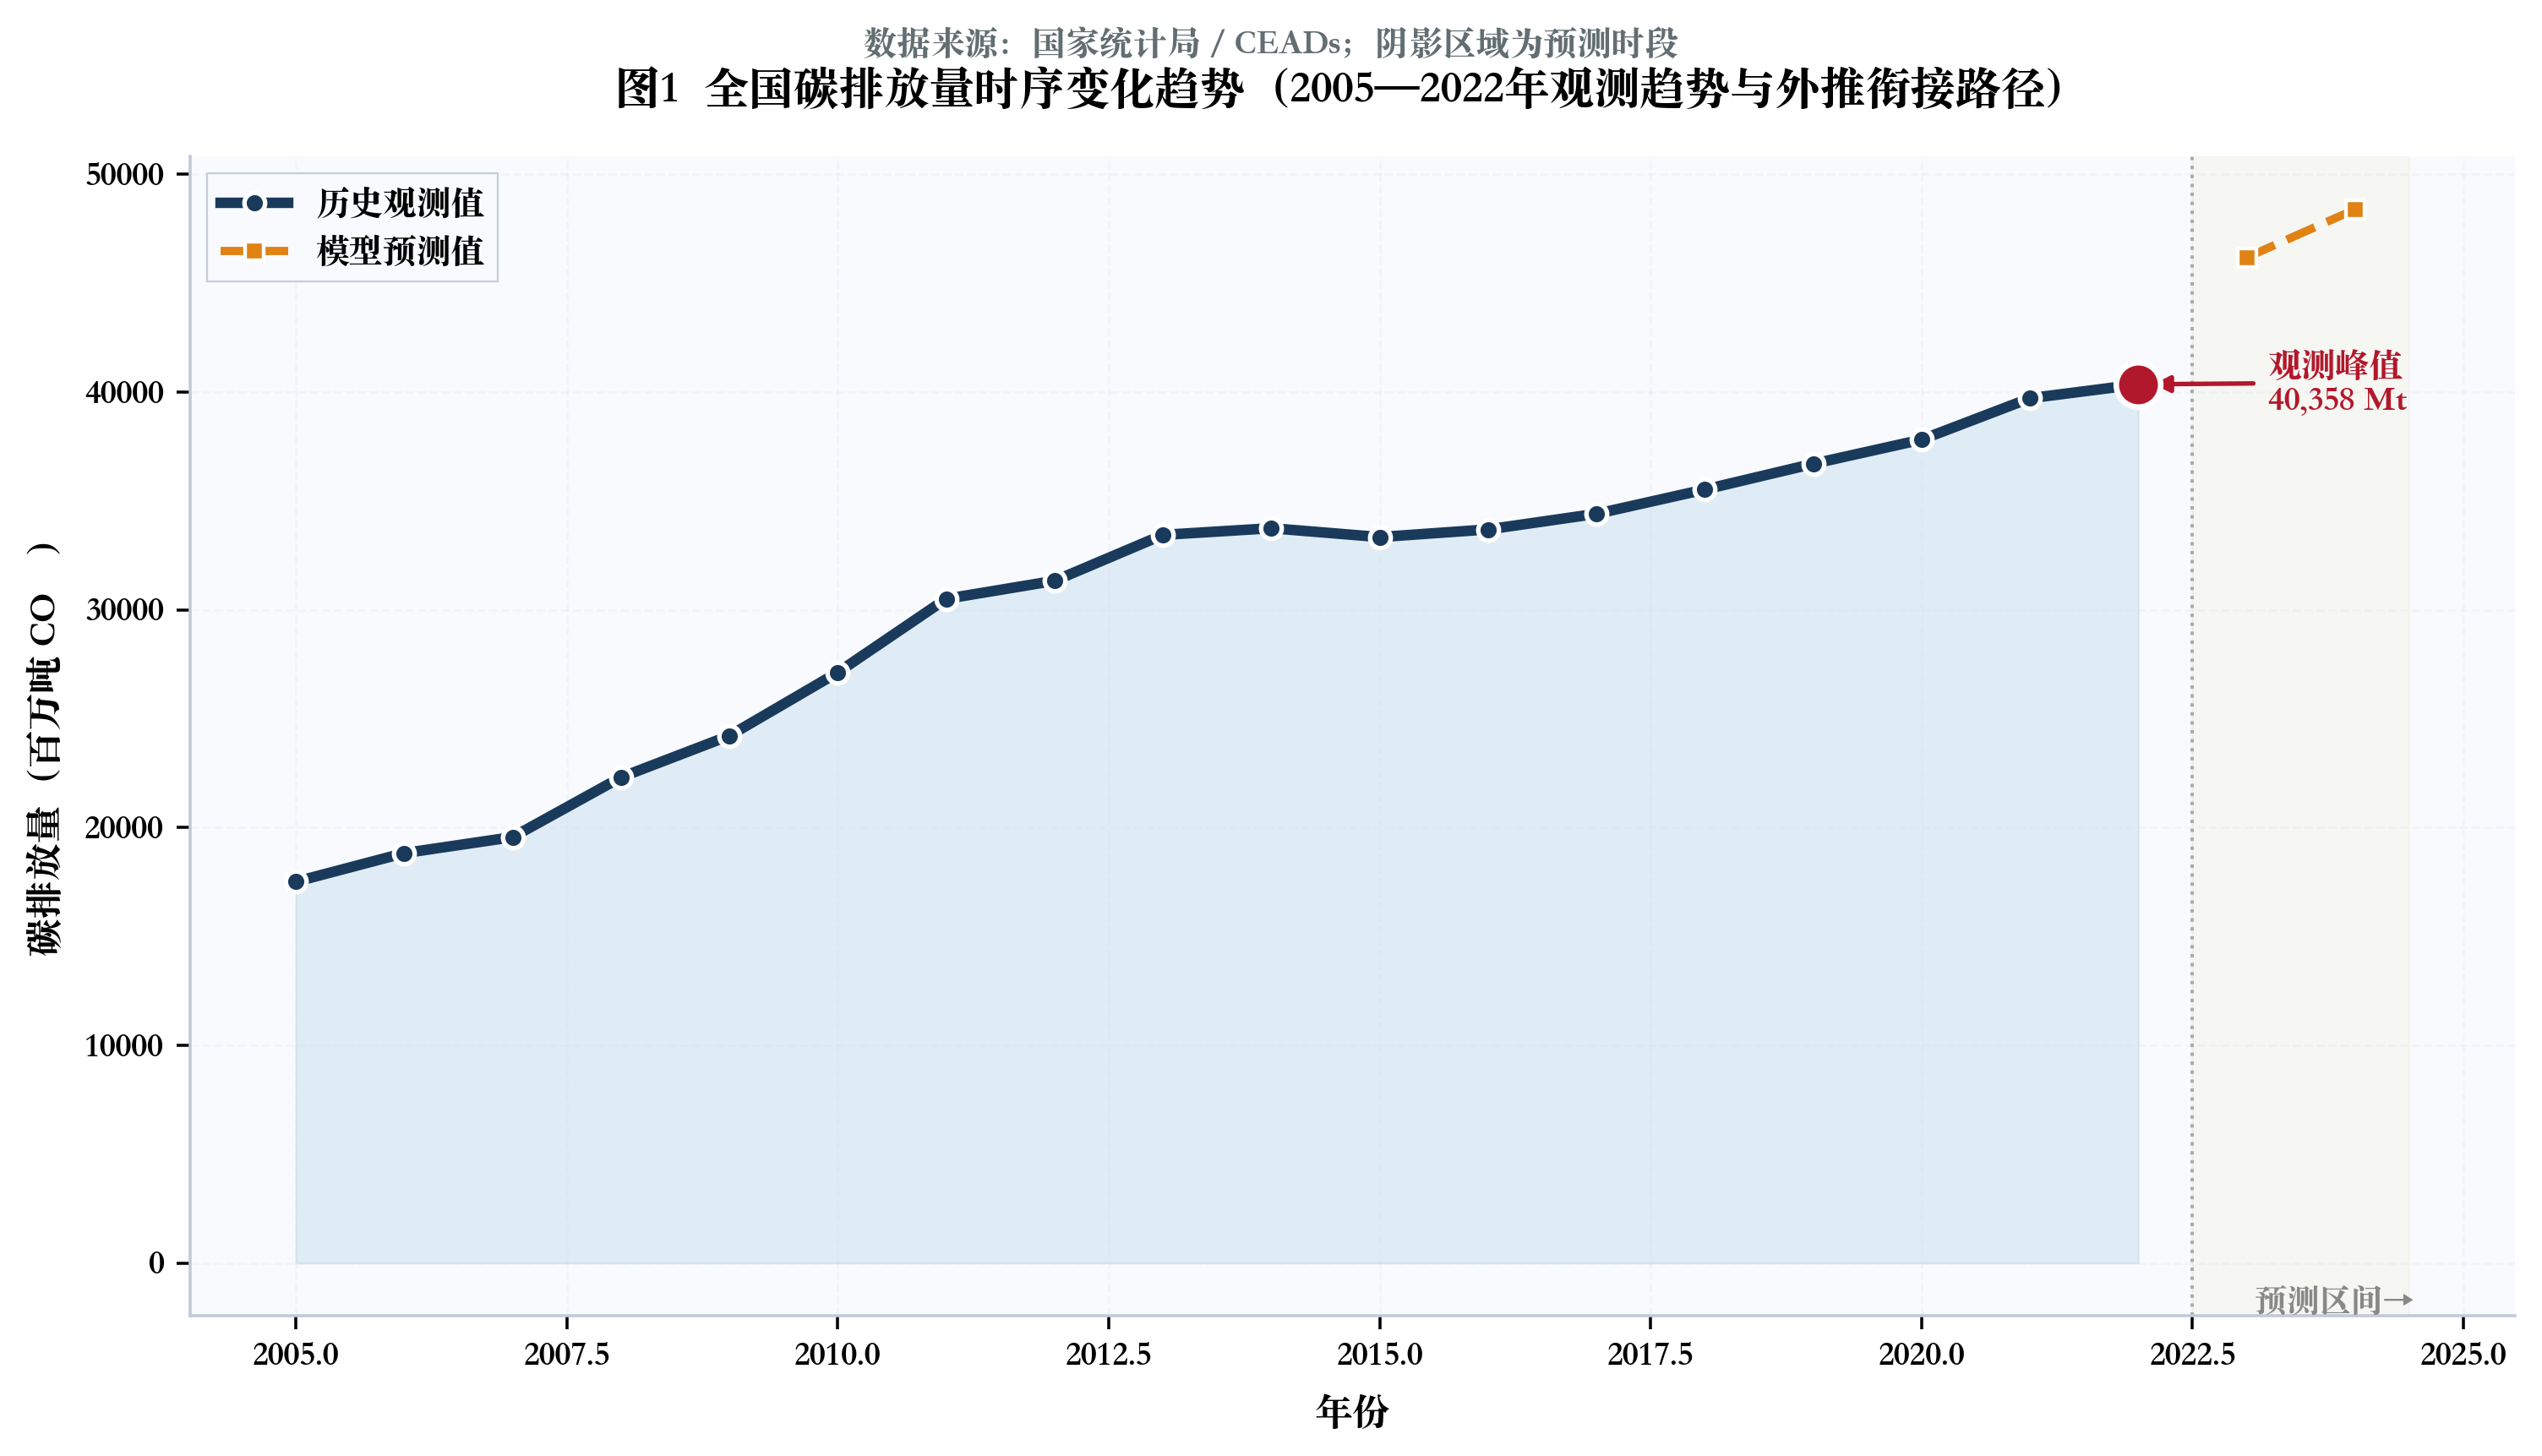
\includegraphics[width=0.82\textwidth]{../outputs/figures/Fig1_national_co2_trend.png}
    \captionof{figure}{2005—2024年中国碳排放总量变化趋势}
    \label{fig:co2_trend}
\end{center}
从图\ref{fig:co2_trend}可以看到，碳排放在样本后段仍保持上行惯性，但斜率较前期明显放缓，说明“总量扩张”与“结构调整”正在并行发生。我国排放路径已由快速爬升阶段逐步转入高位调整阶段，后续峰值形态将更受能源与产业结构变化影响。

\begin{center}
    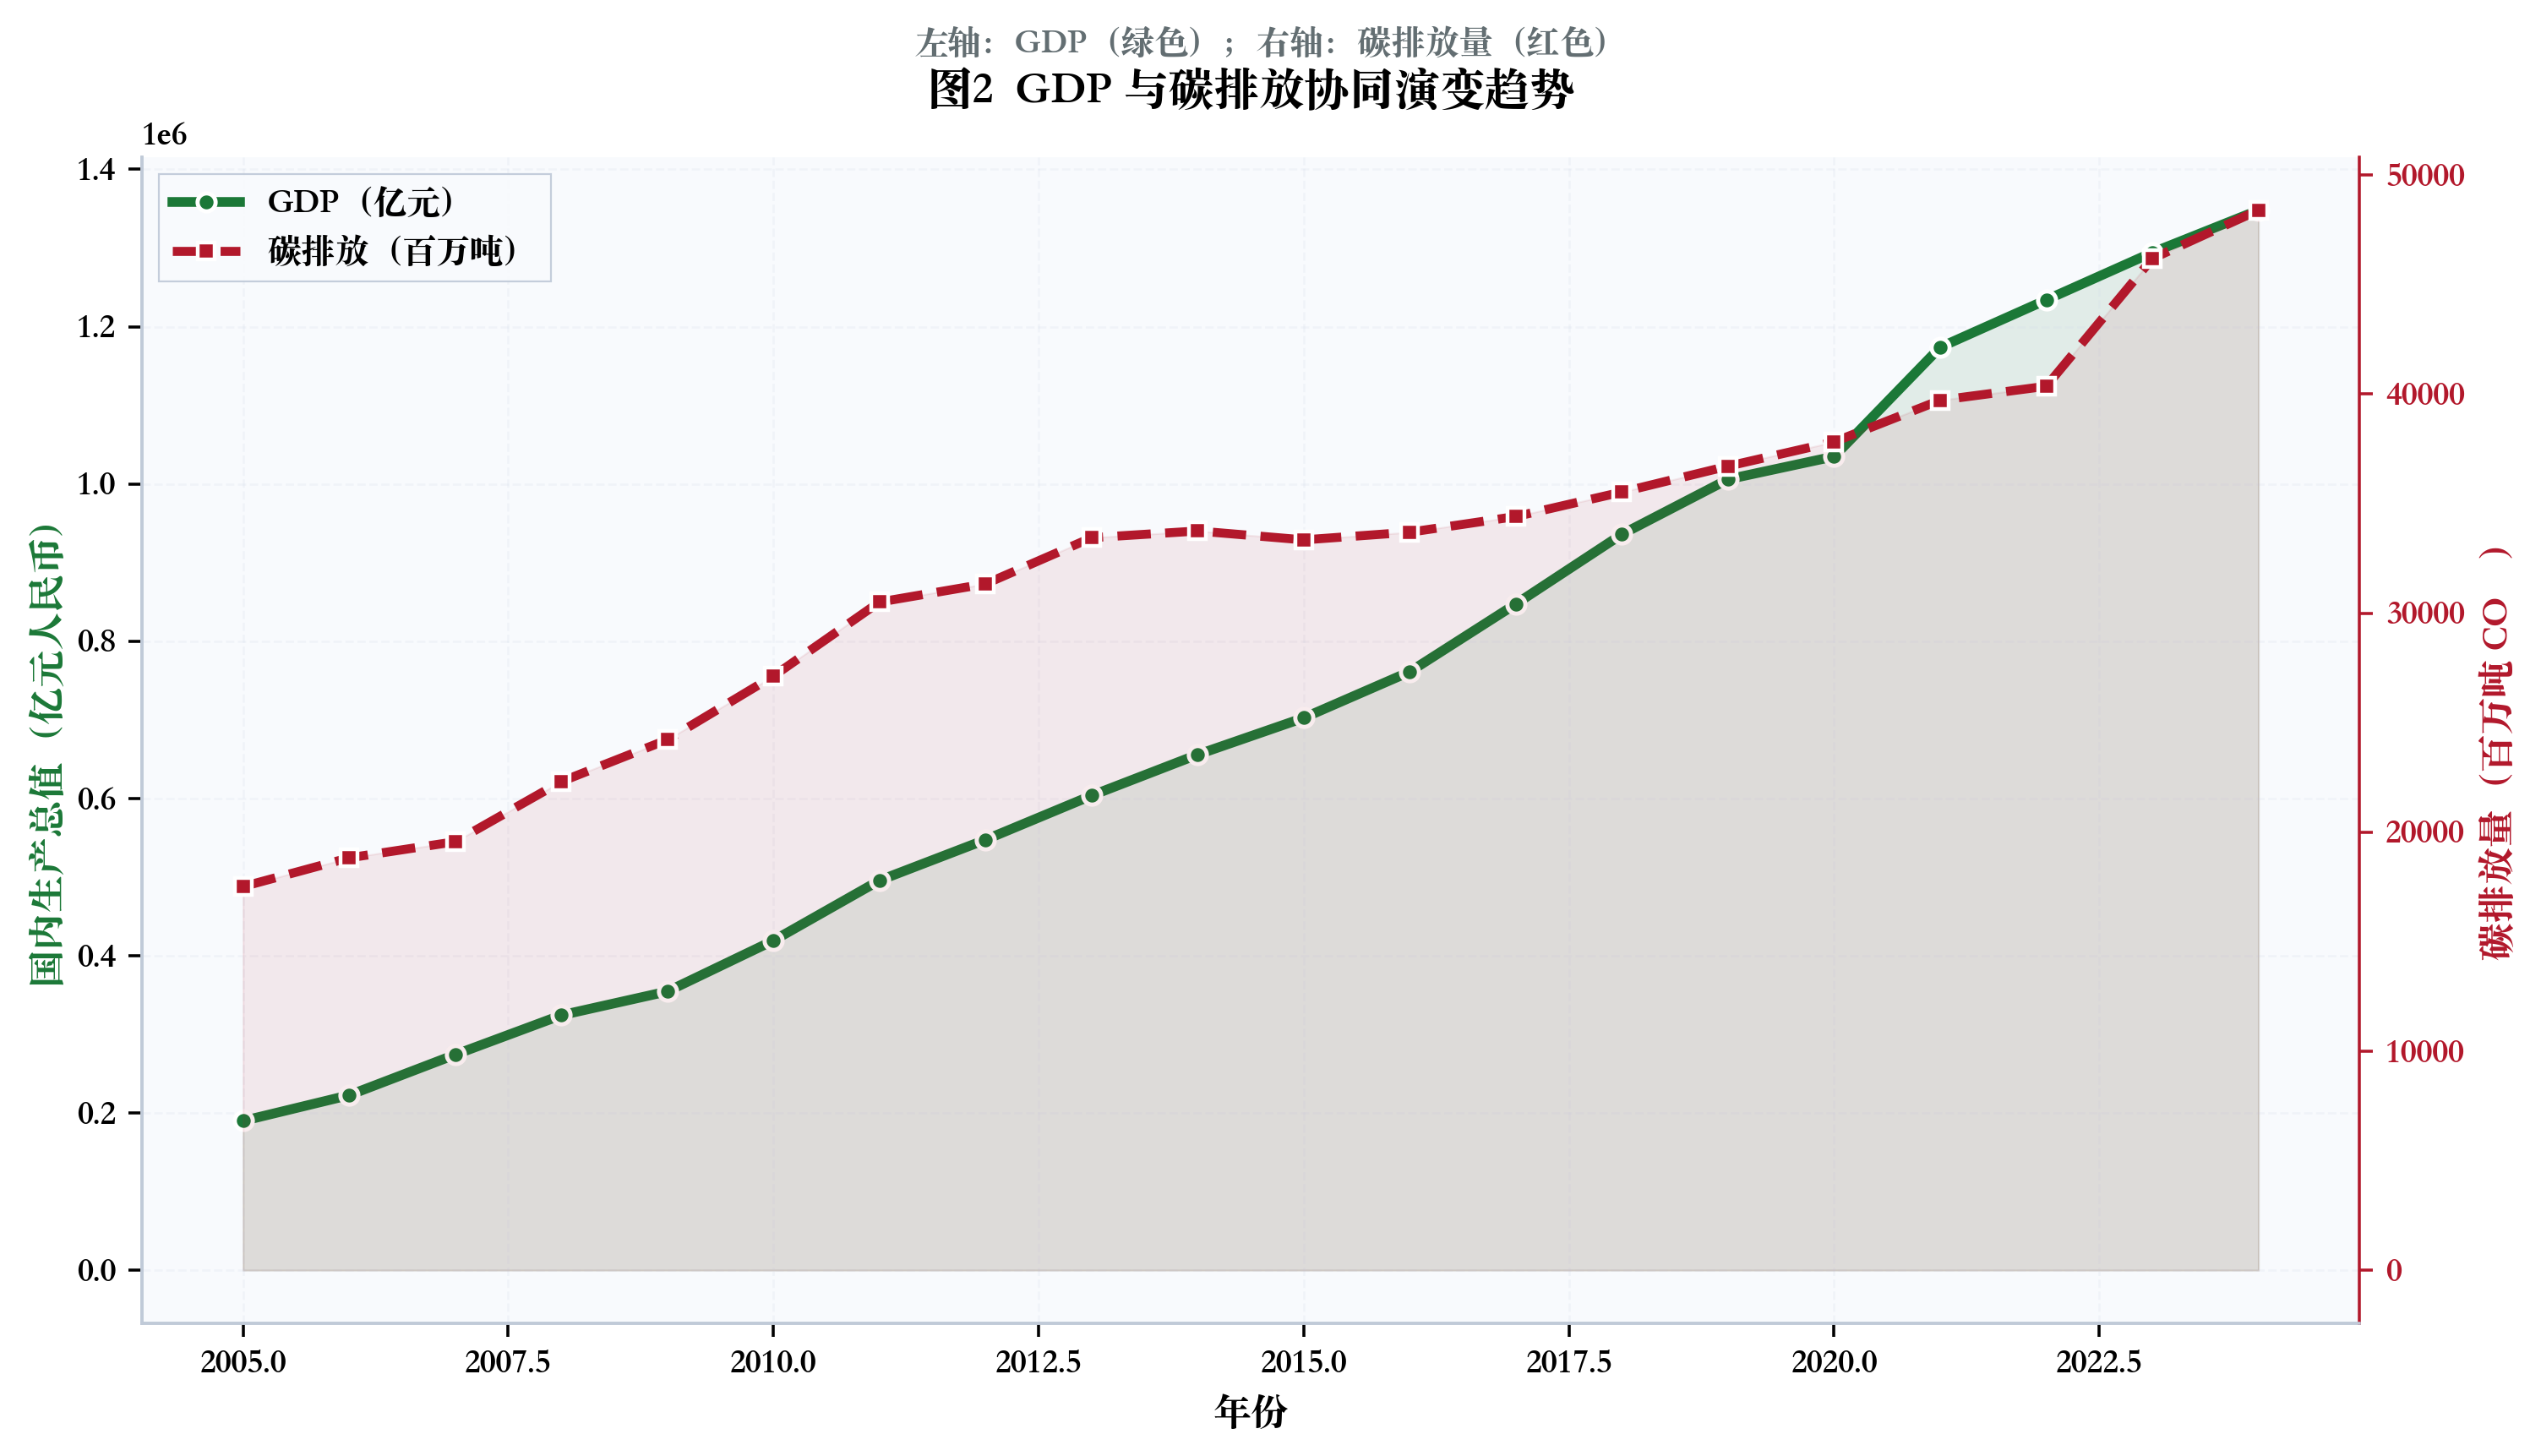
\includegraphics[width=0.86\textwidth]{../outputs/figures/Fig2_gdp_co2_dual_axis.png}
    \captionof{figure}{2005—2024年GDP与碳排放双轴对比}
    \label{fig:gdp_co2}
\end{center}
图\ref{fig:gdp_co2}表明，GDP与碳排放长期同向变化，但并非同比例同步增长。后期经济总量继续扩张而排放增速趋缓，反映增长方式正由高碳要素驱动向效率与结构驱动过渡。

\begin{center}
    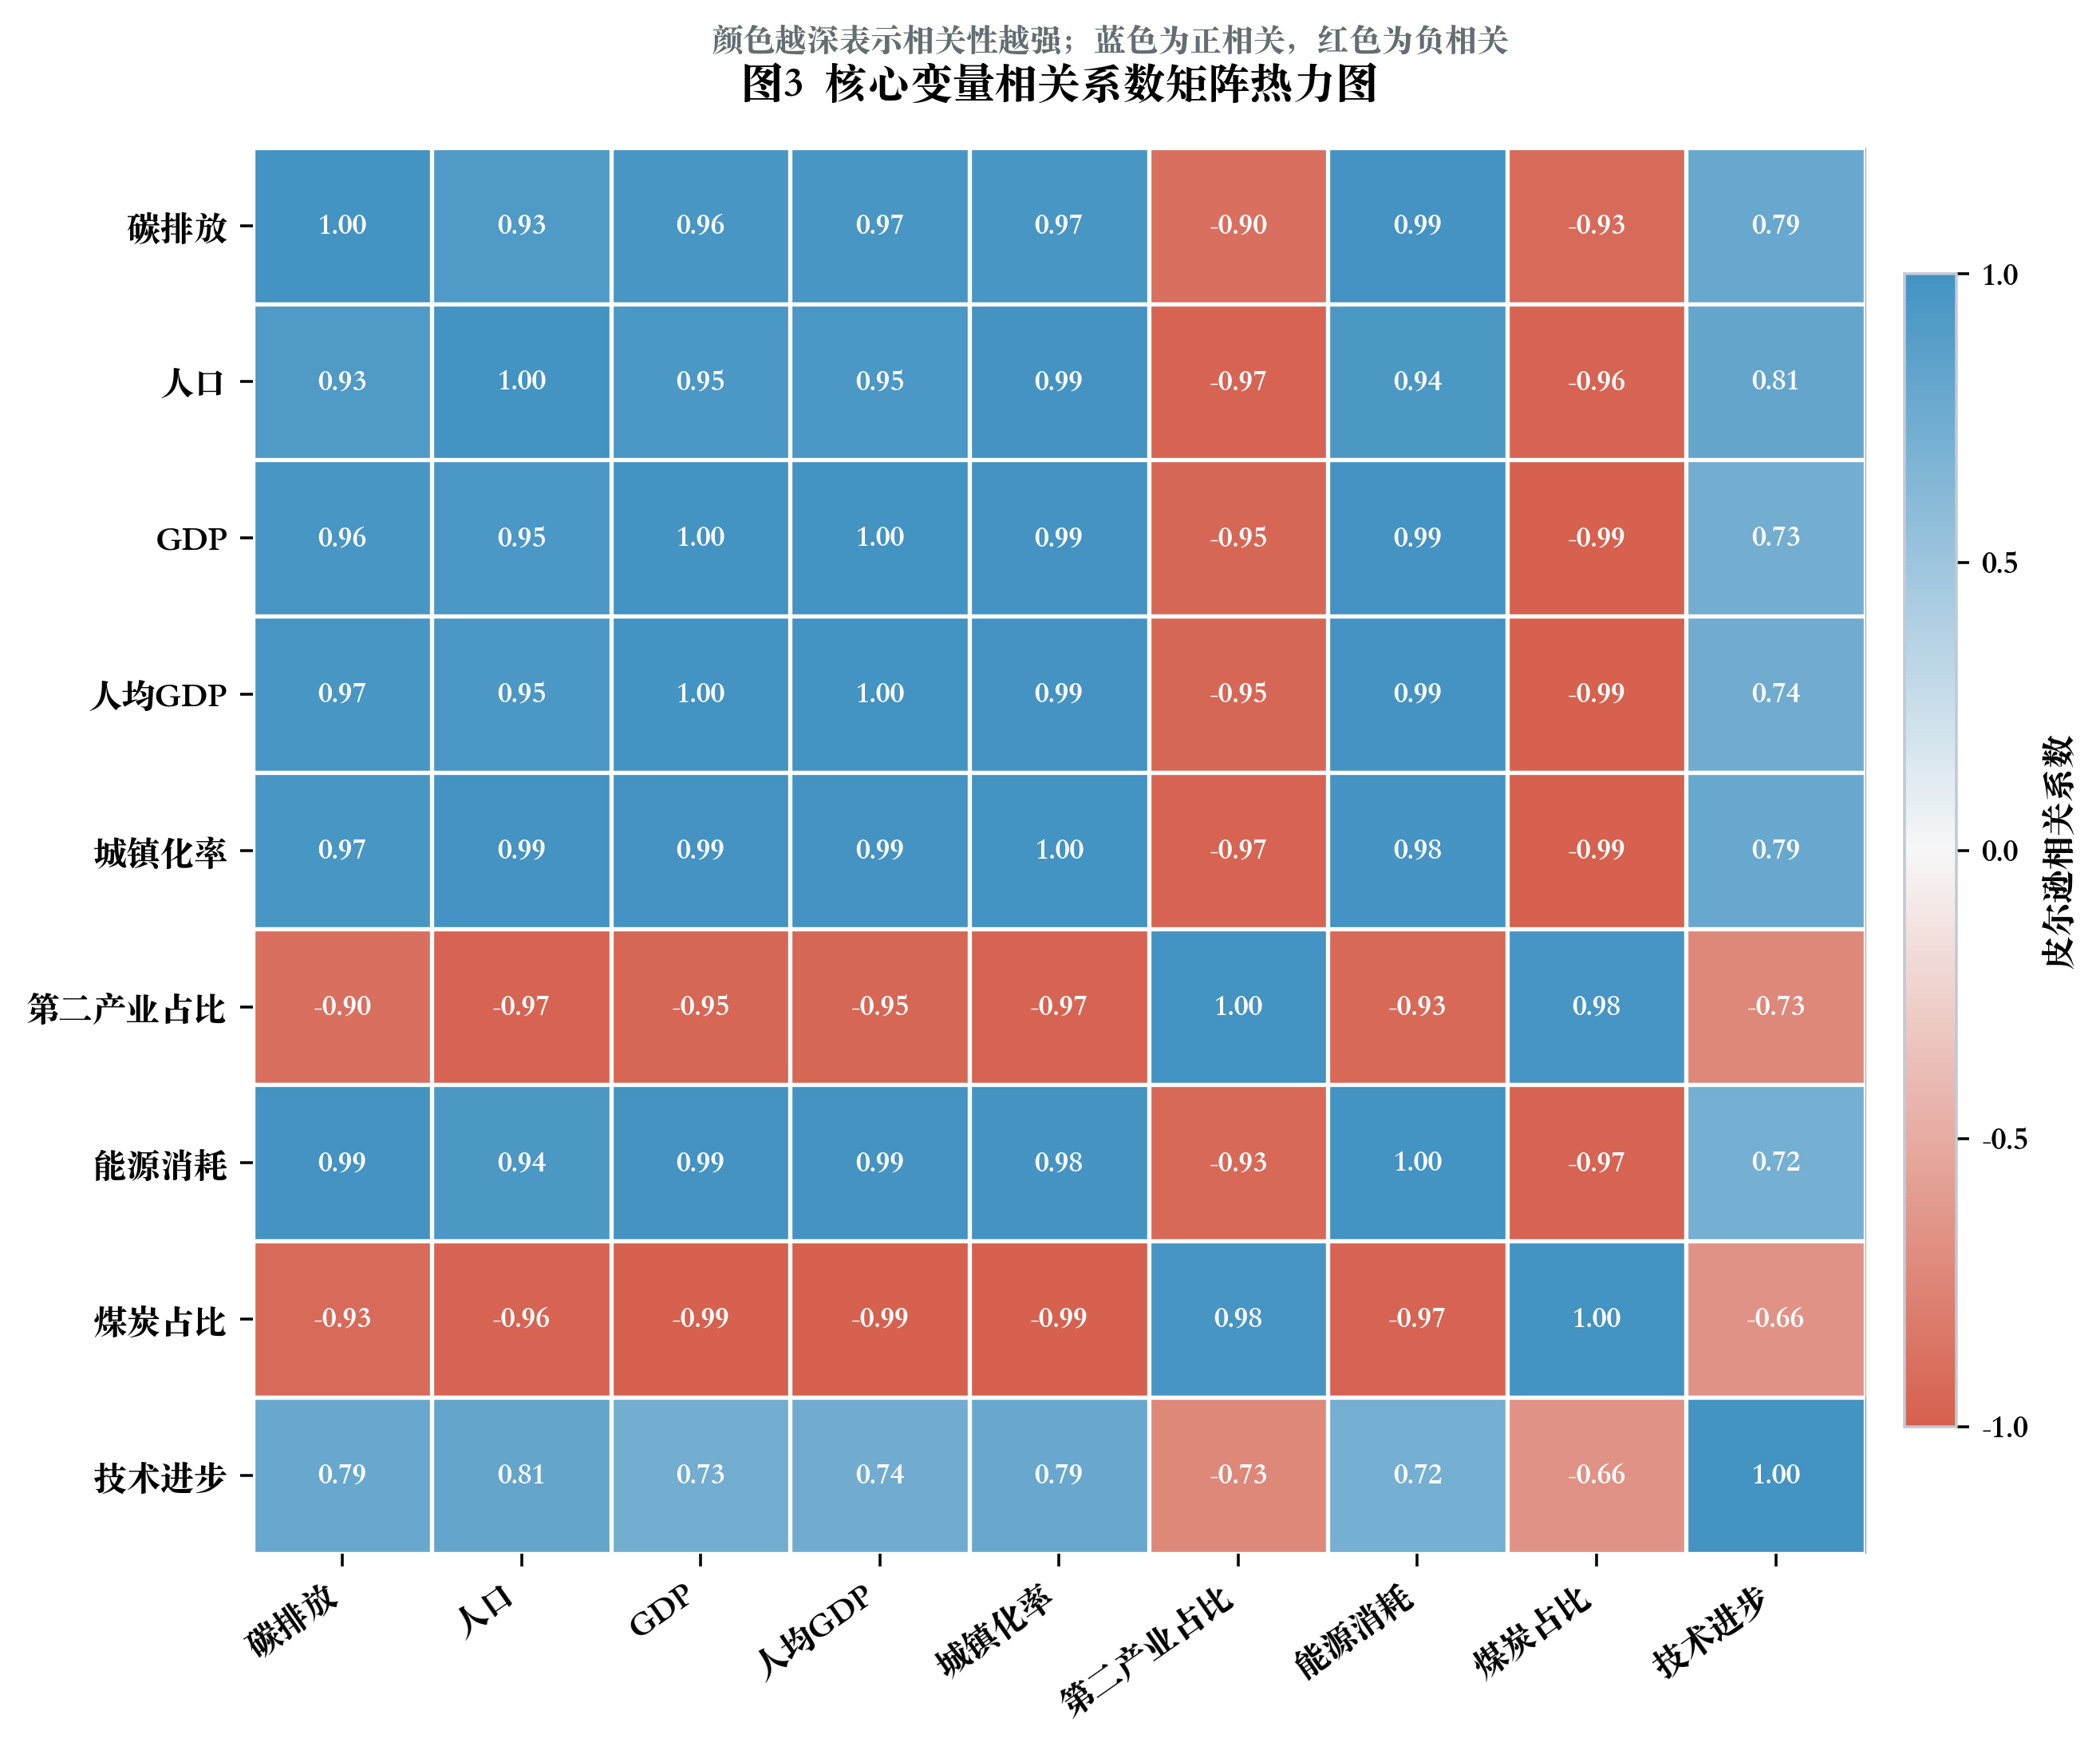
\includegraphics[width=0.78\textwidth]{../outputs/figures/Fig3_correlation_matrix.png}
    \captionof{figure}{核心变量相关性矩阵热力图}
    \label{fig:corr}
\end{center}
从图\ref{fig:corr}所示相关结构看，能源消费、GDP等规模变量与碳排放总体呈正相关；煤炭占比下降、产业升级与减排方向更一致。这一统计特征为后续参数设定提供了依据。

\begin{center}
    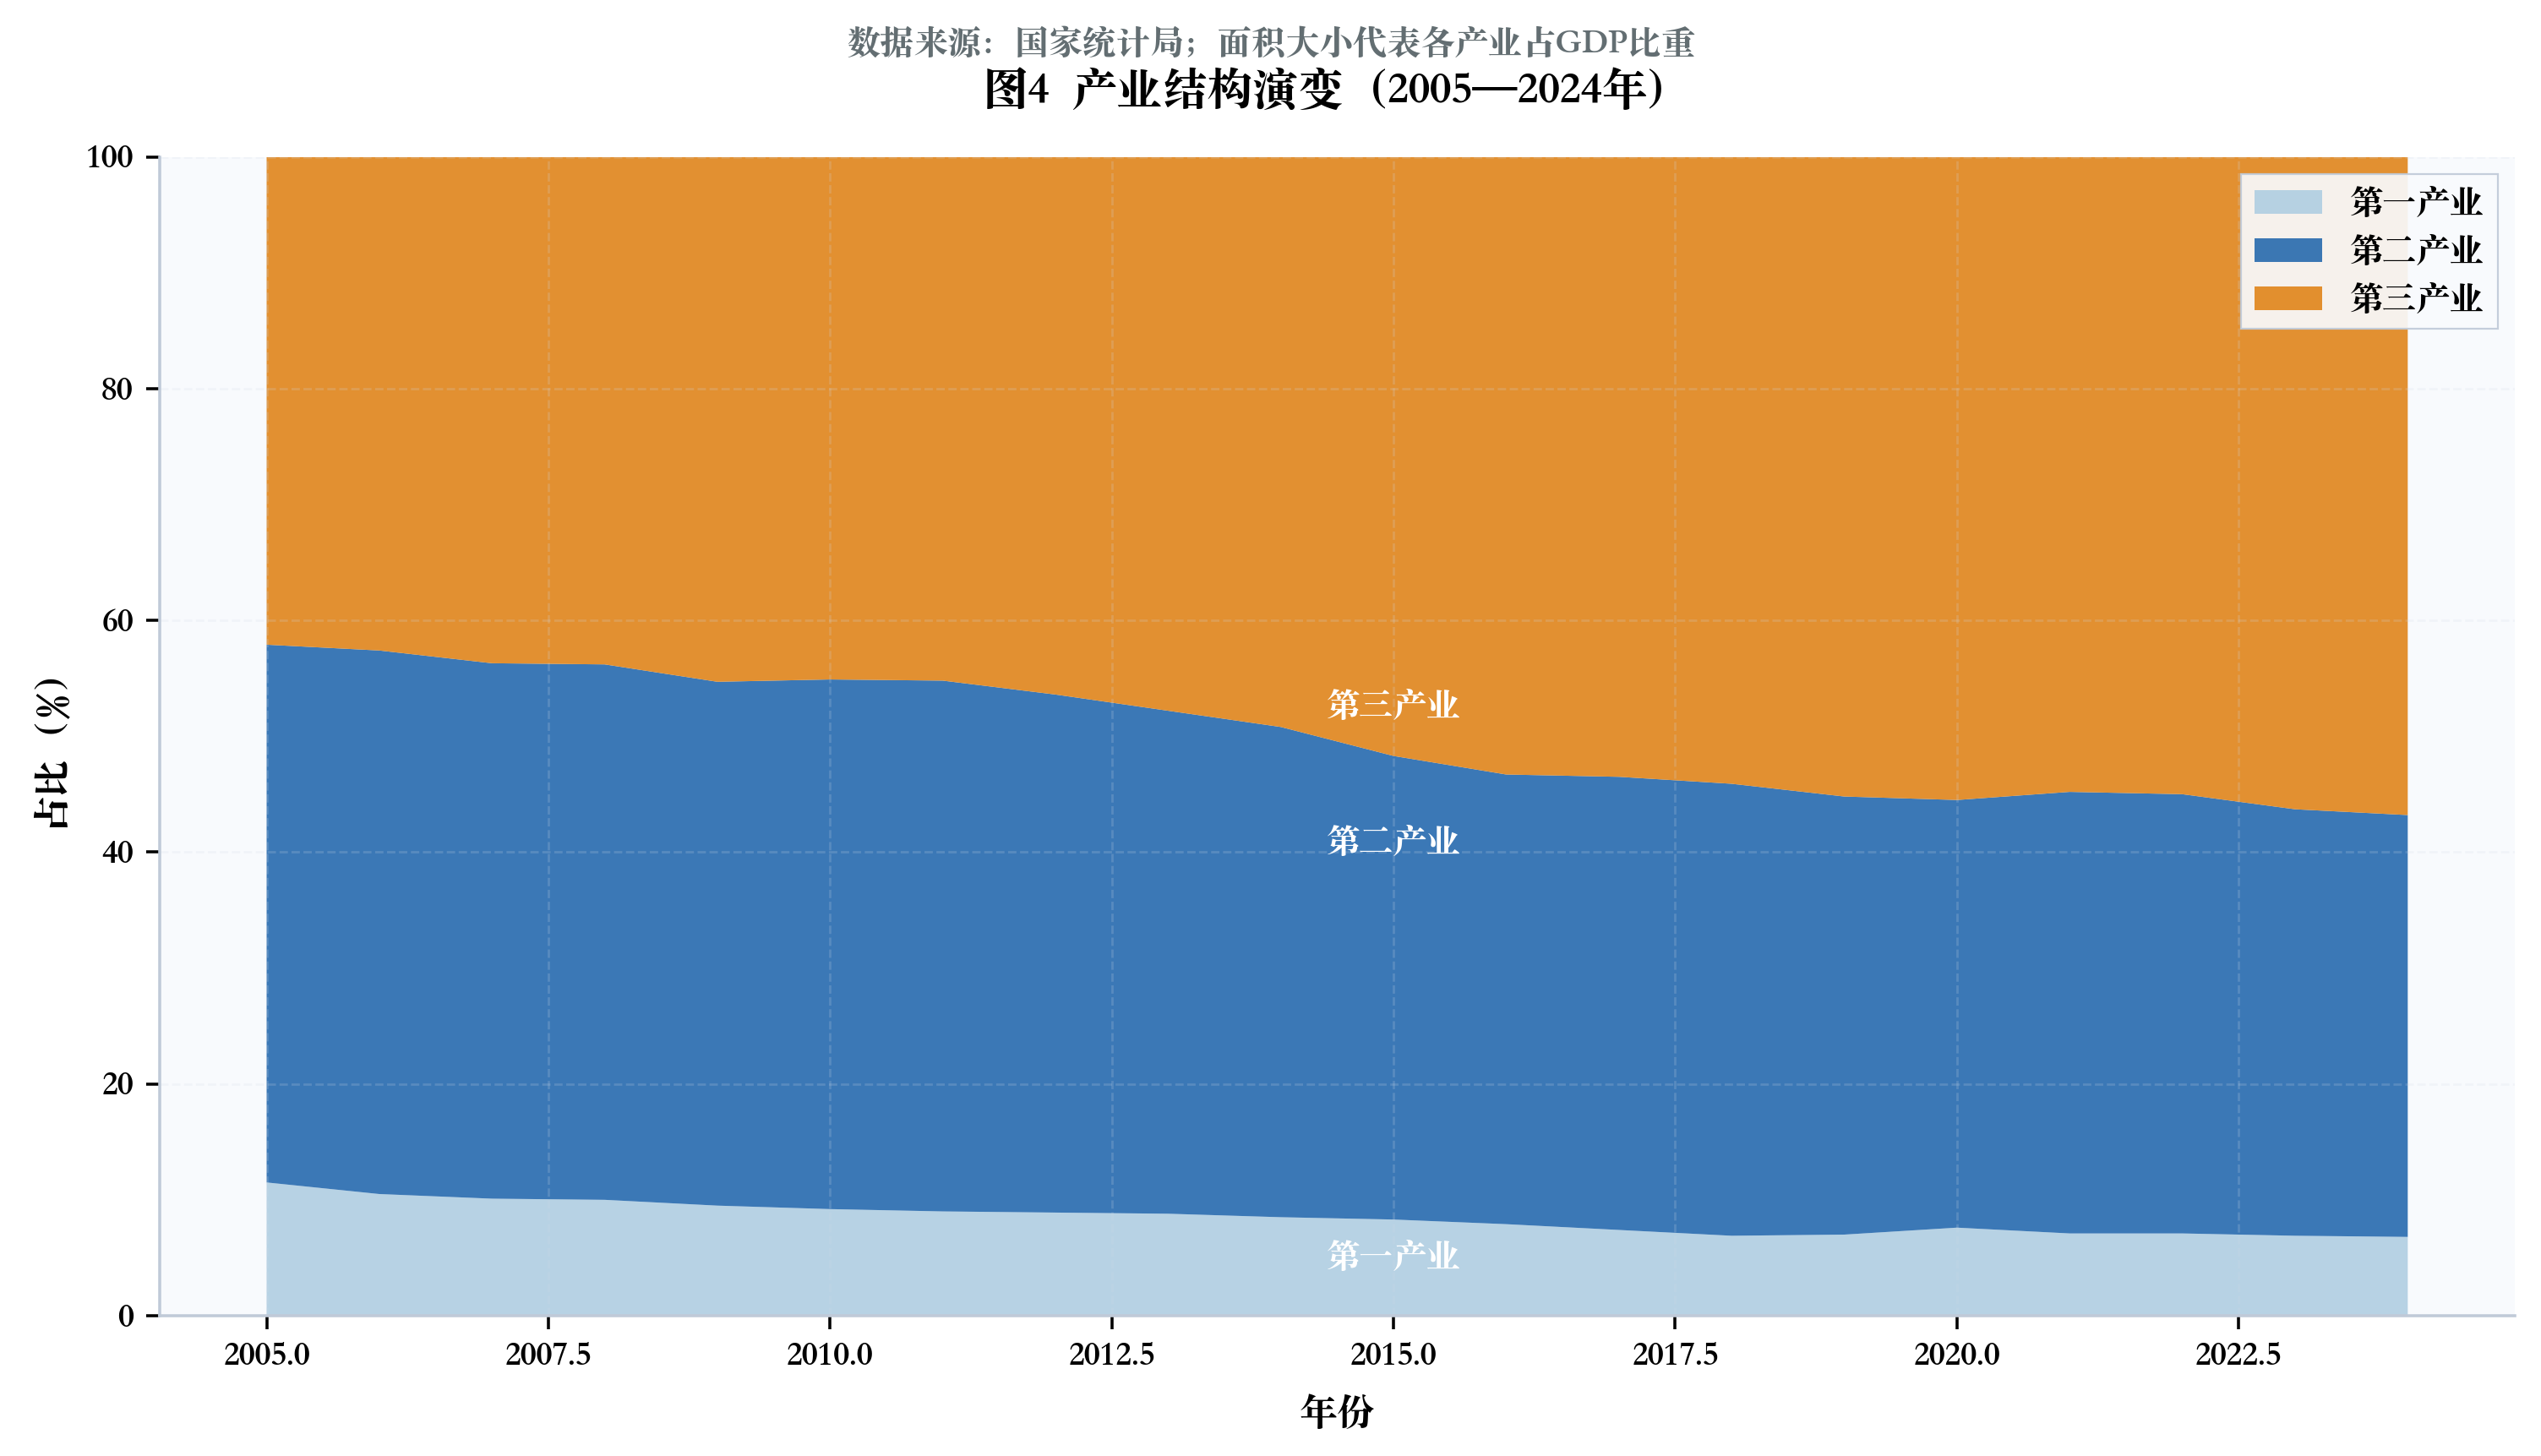
\includegraphics[width=0.84\textwidth]{../outputs/figures/Fig4_industry_structure.png}
    \captionof{figure}{产业结构演化趋势图}
    \label{fig:industry_structure}
\end{center}
结合图\ref{fig:industry_structure}可见，第二产业占比总体下降、第三产业占比上升，是样本期内排放增速放缓的重要背景。这并不意味着工业作用消失，而是说明工业内部升级与服务业扩张共同改变了单位产出对应的排放强度。

\begin{center}
    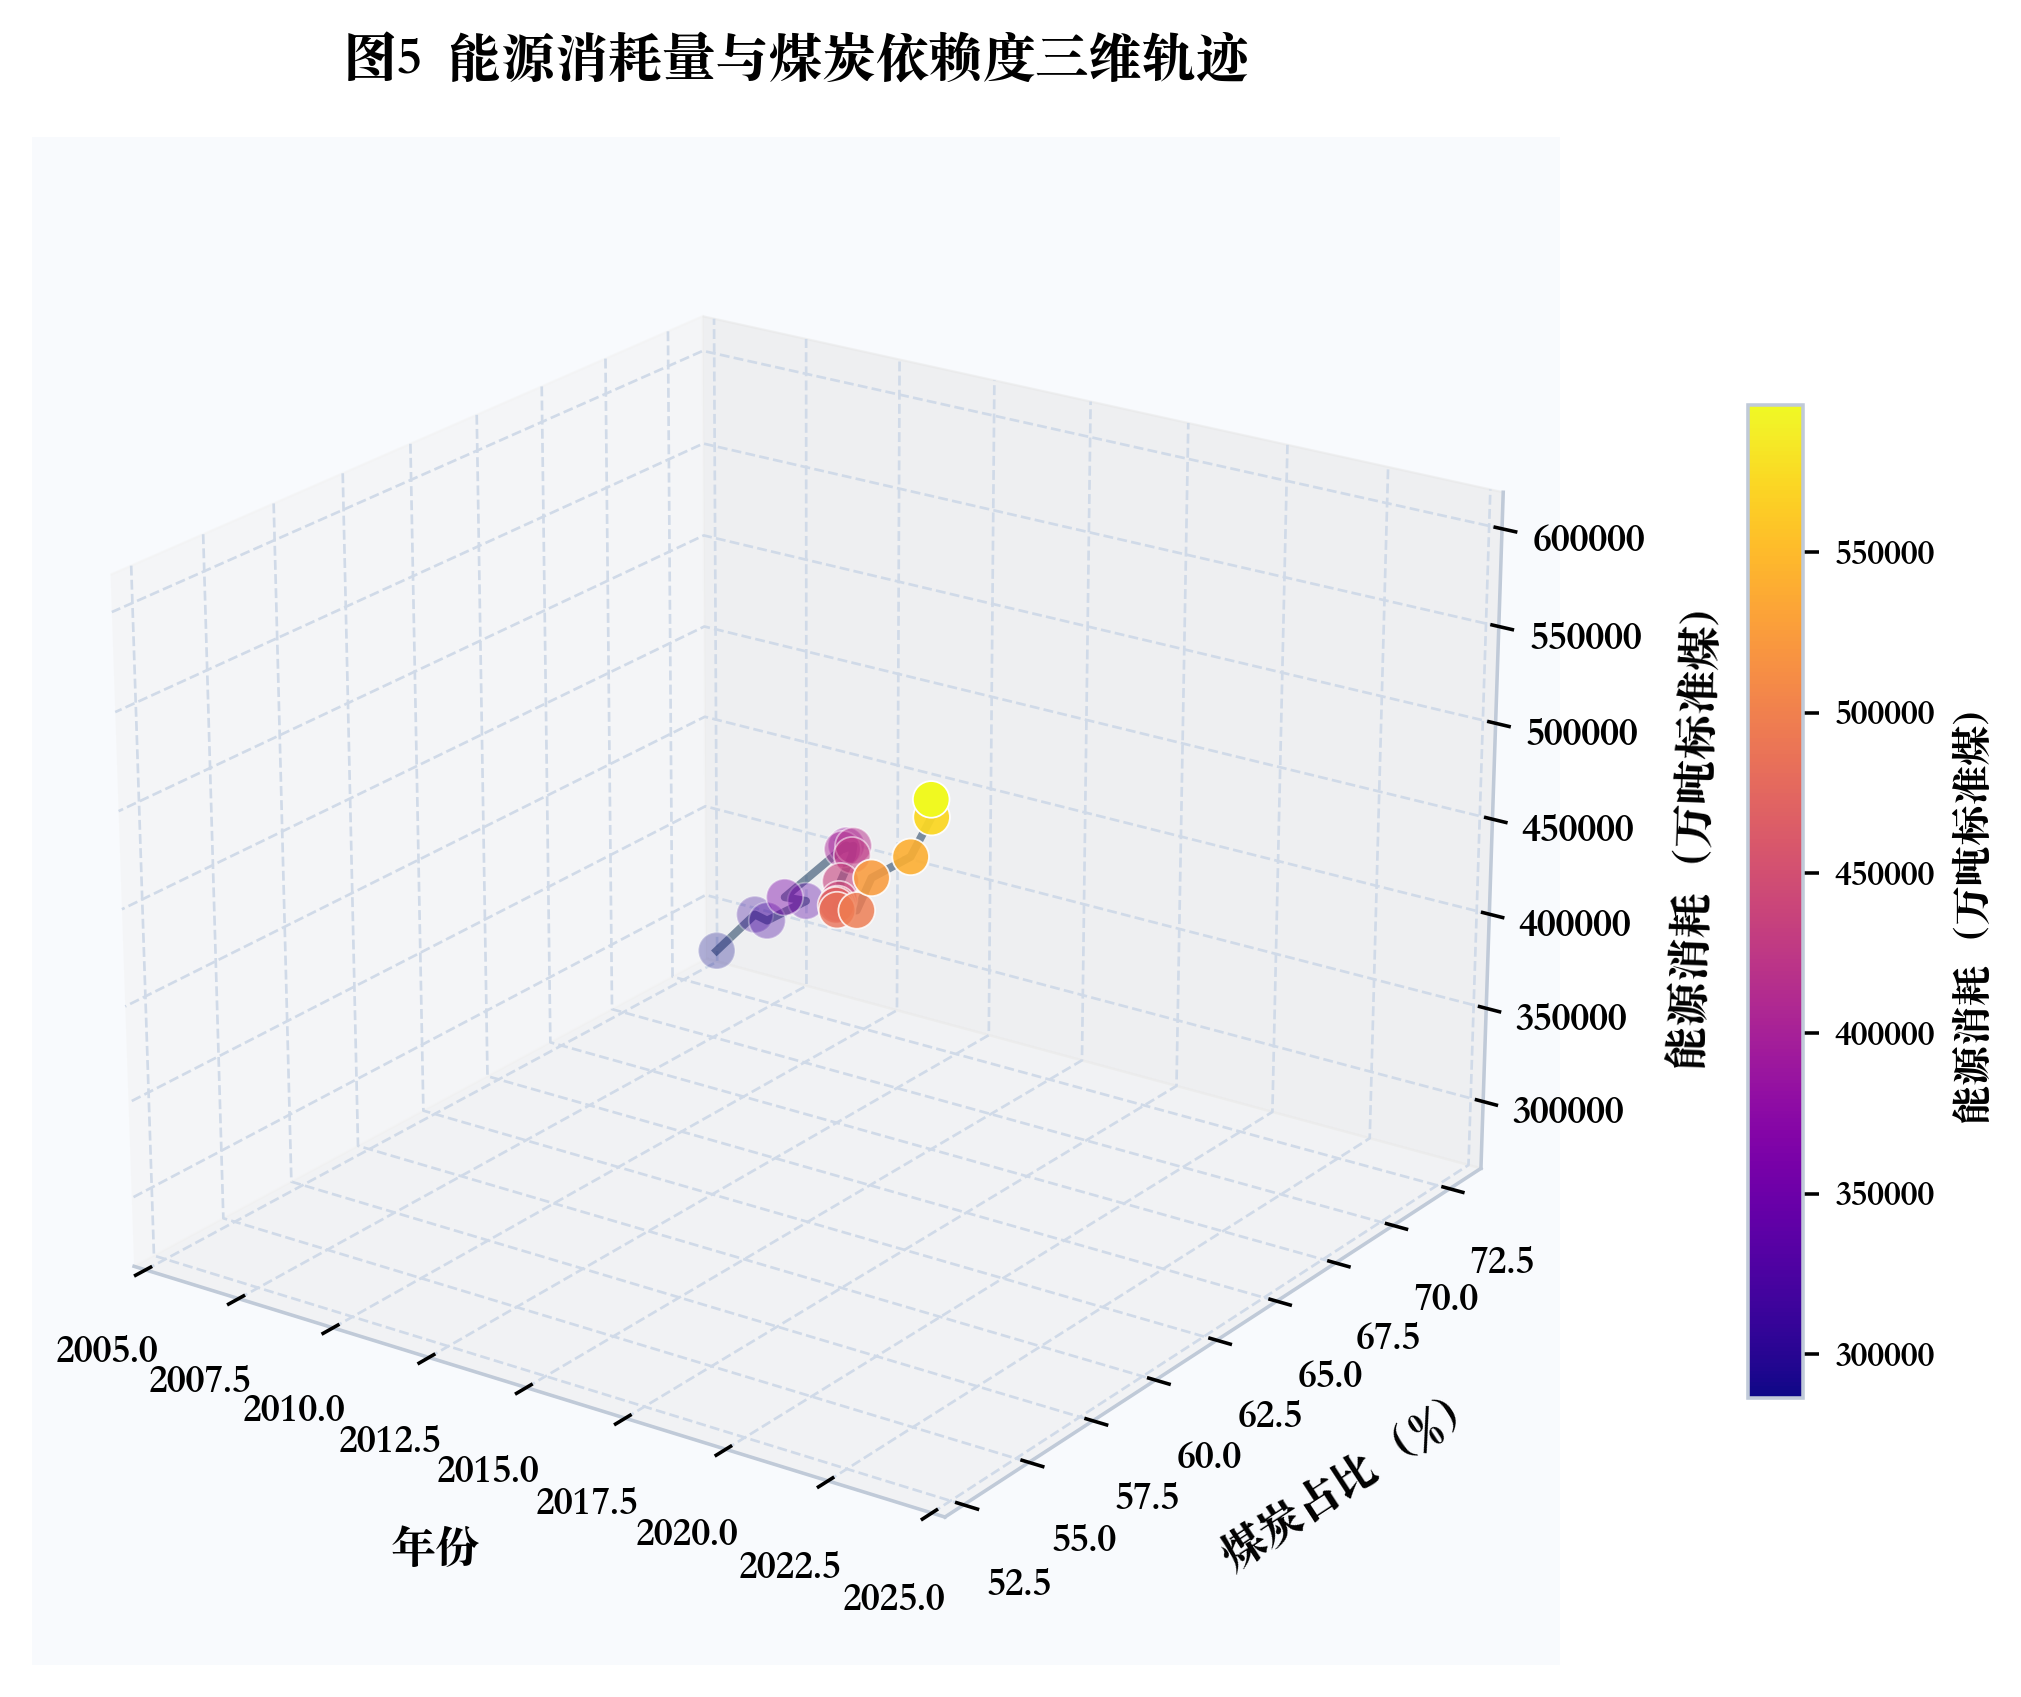
\includegraphics[width=0.82\textwidth]{../outputs/figures/Fig5_energy_structure.png}
    \captionof{figure}{能源总量与煤炭依赖三维联动图}
    \label{fig:energy_structure}
\end{center}
图\ref{fig:energy_structure}展示了“年份—煤炭依赖—能源总量”的联动关系：能源总量仍处高位，而煤炭占比持续下降。这说明我国处于“总量约束尚强、结构改善先行”的过渡阶段，也解释了为什么短期内排放难以快速下行，但中长期可通过结构优化压低峰值。

\begin{center}
    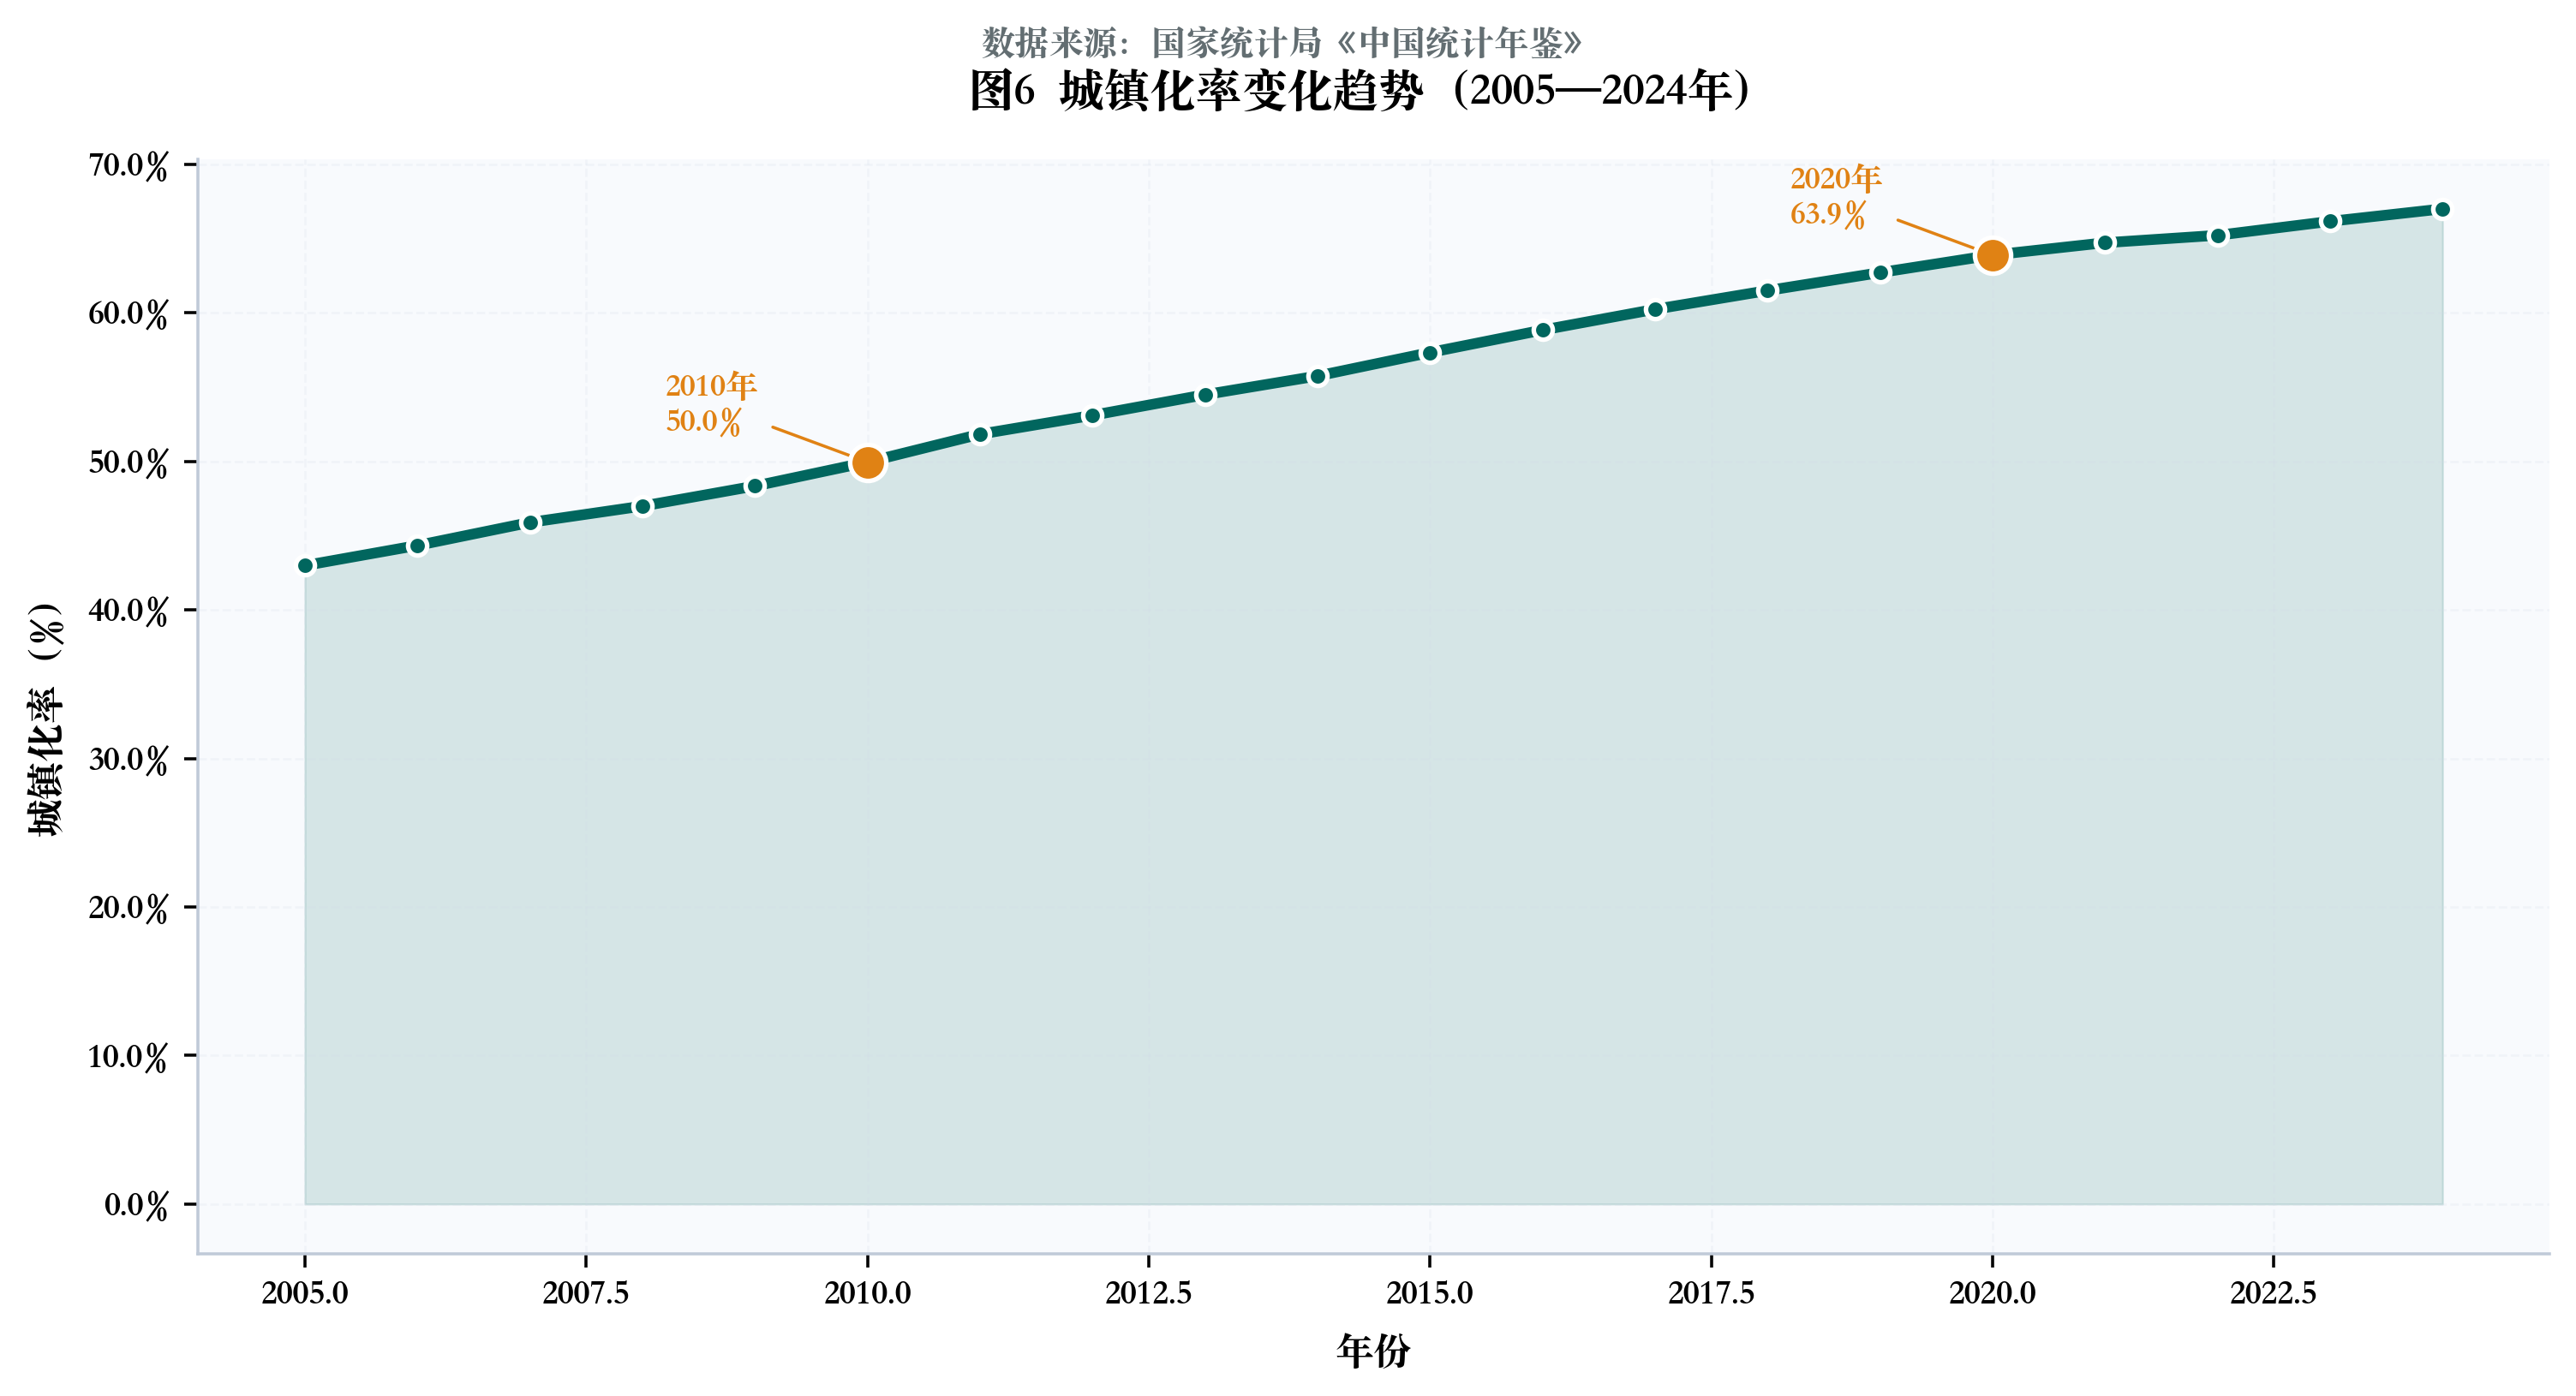
\includegraphics[width=0.82\textwidth]{../outputs/figures/Fig6_urbanization_rate.png}
    \captionof{figure}{城镇化率变化趋势}
    \label{fig:urbanization_rate}
\end{center}
由图\ref{fig:urbanization_rate}可知，城镇化率持续上升，但城镇化并不必然推高排放。若公共服务效率、基础设施集约利用和技术扩散同步提升，城镇化可能转化为减排效率提升通道。

\subsection{驱动机制识别}
在总体趋势基础上，本节通过EKC检验、扩展STIRPAT估计和中介分析识别“经济—能源—结构—技术”的作用链。

\begin{center}
    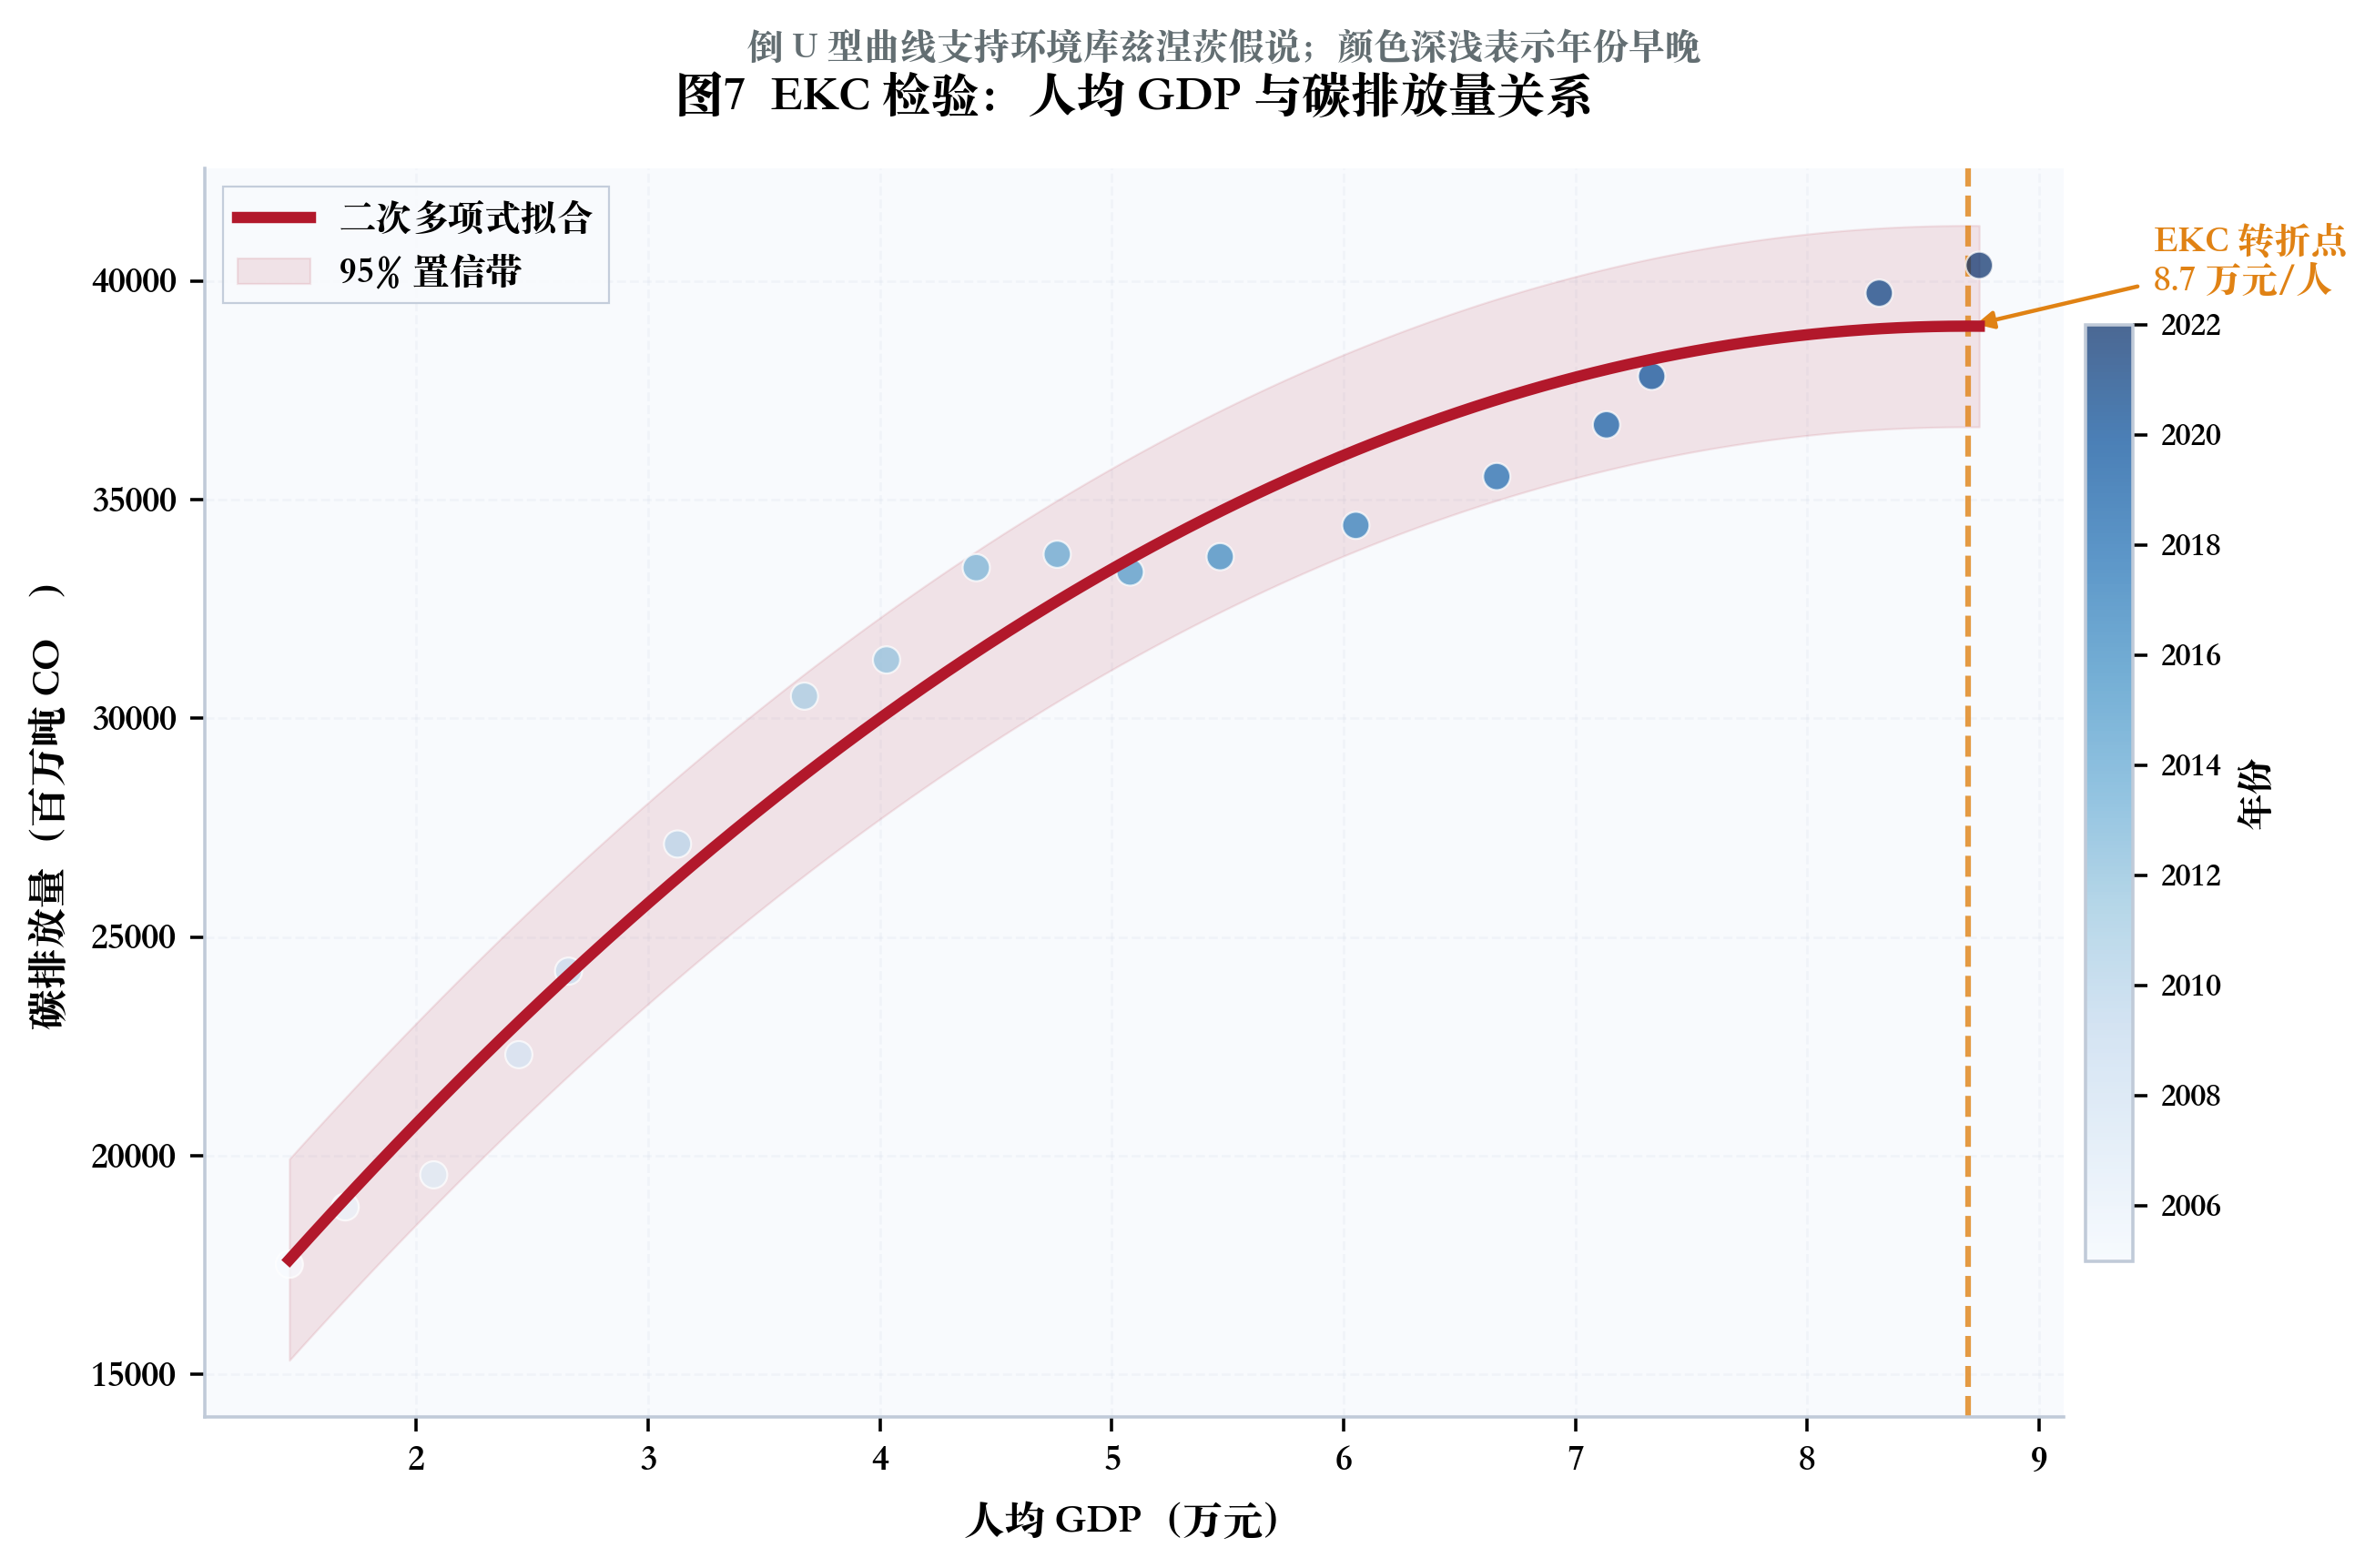
\includegraphics[width=0.72\textwidth]{../outputs/figures/Fig7_ekc_scatter_fit.png}
    \captionof{figure}{EKC检验：人均GDP与碳排放关系}
    \label{fig:ekc}
\end{center}
从图\ref{fig:ekc}可以看出，人均GDP与碳排放之间存在显著非线性关系，说明排放演化并非简单线性过程，而是进入受产业升级与能源替代共同影响的阶段性转型区间。


\begin{center}
    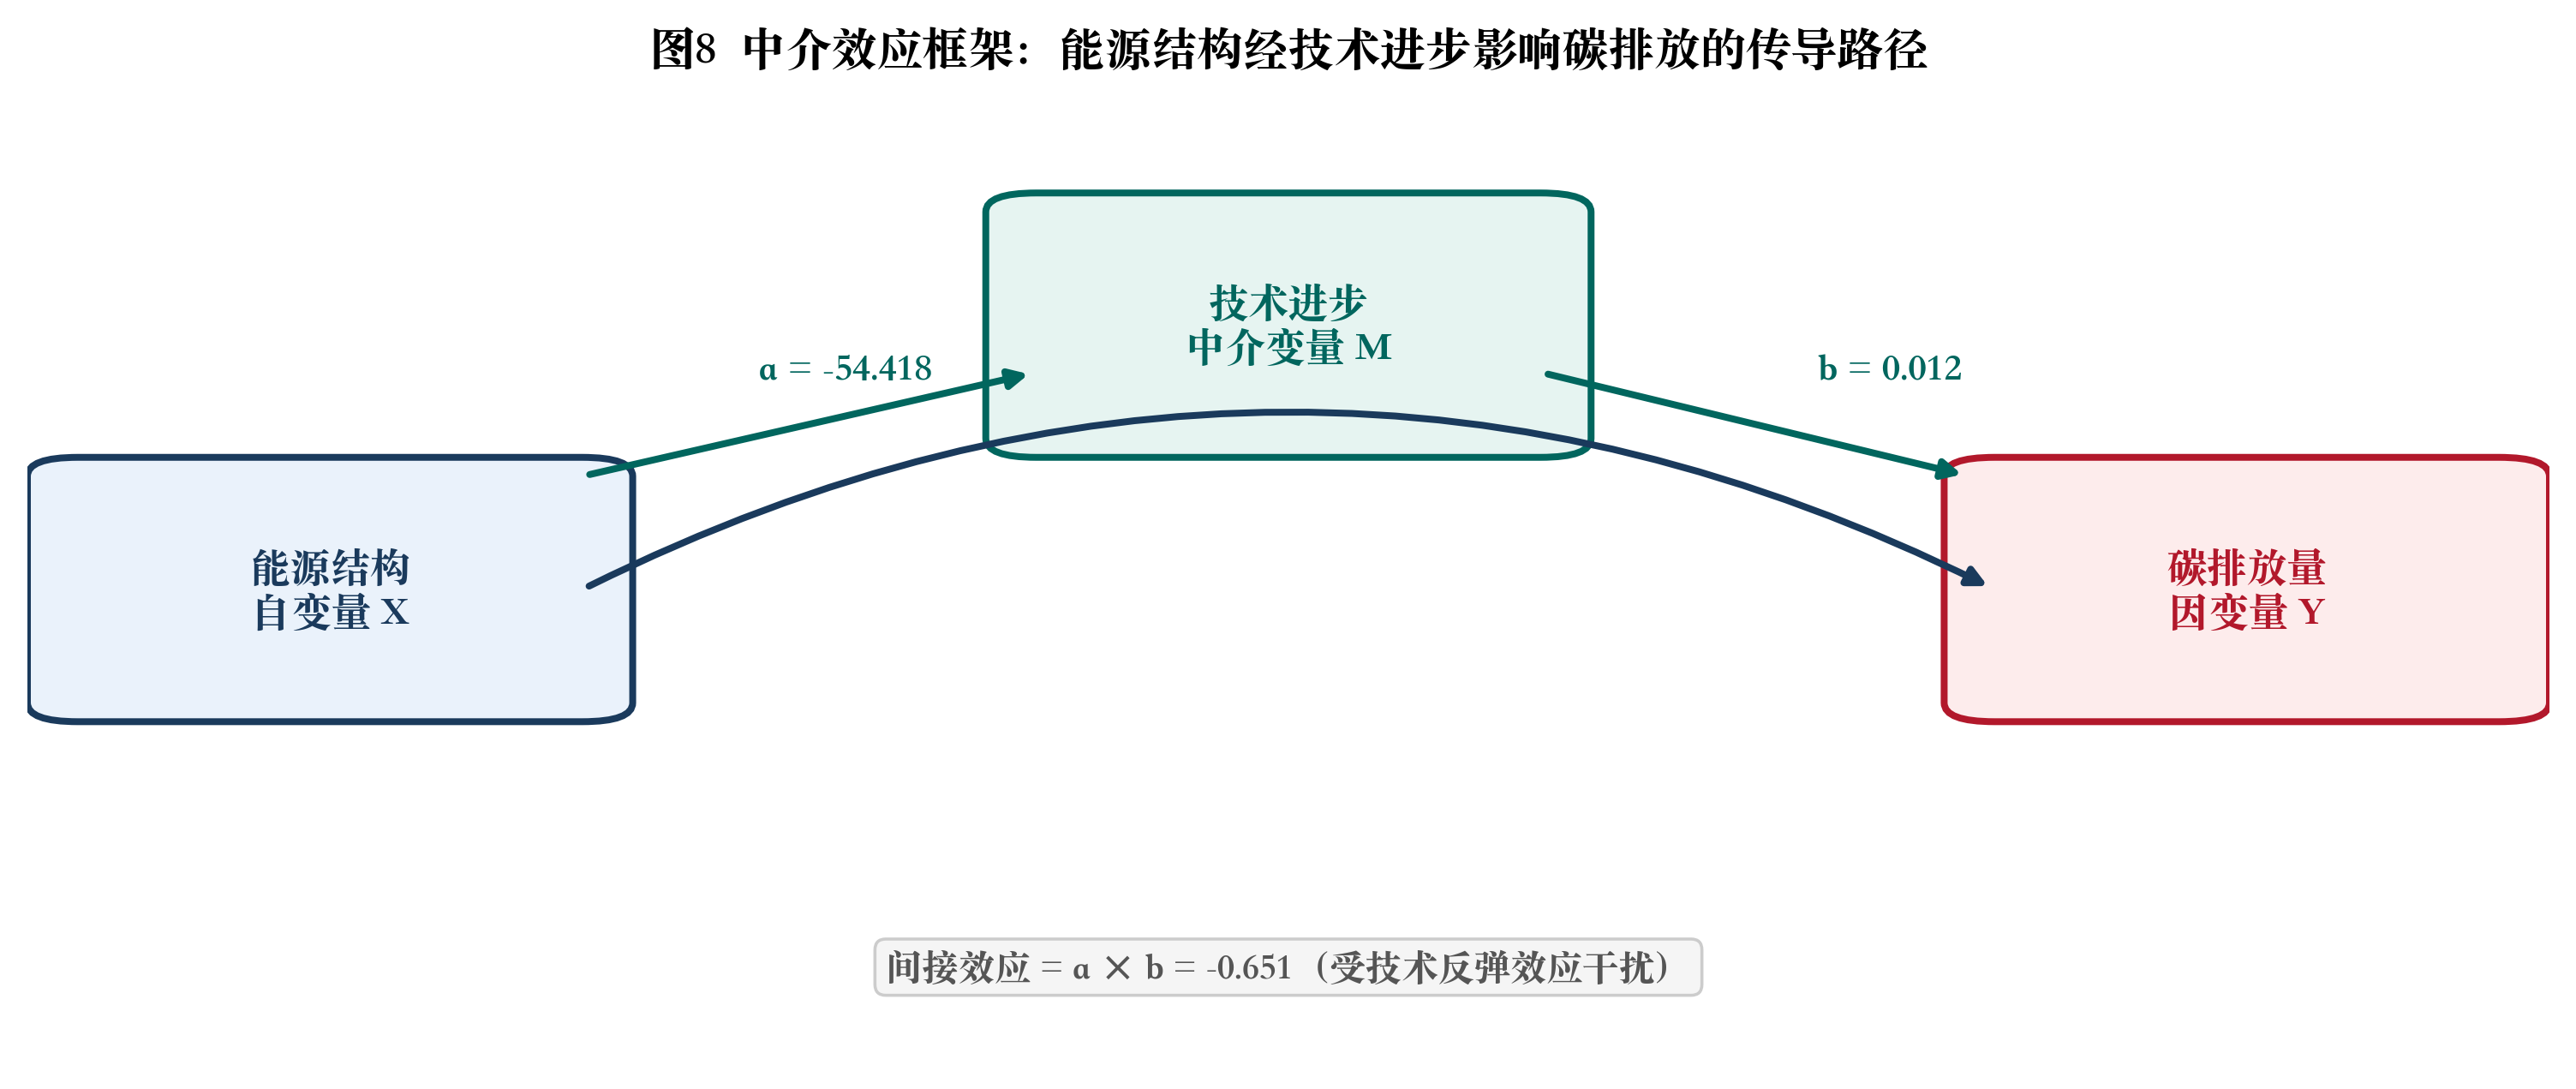
\includegraphics[width=0.84\textwidth]{../outputs/figures/Fig8_mediation_framework.png}
    \captionof{figure}{中介效应路径示意图}
    \label{fig:mediation}
\end{center}
图\ref{fig:mediation}揭示了能源结构对碳排放的复杂传导路径。值得注意的是，在未控制经济规模的单方程回归中，煤炭占比的总效应系数呈负向。这主要是受样本期内GDP与煤炭占比反向变动趋势的干扰。在剥离规模效应后，其直接效应转为显著正向，这进一步说明了前文扩展 STIRPAT 模型中多变量联合控制的必要性。

从中介链条来看，煤炭占比对技术进步（a 路径）具有显著的负向压制（$a = -54.42$），说明高煤耗路径在一定程度上挤出了创新要素积累；而技术进步对排放的影响（b 路径）在控制 GDP 后表现为极微弱的正向（$b = 0.012$），间接效应（$a \times b = -0.65$）虽为负，但绝对量远小于直接效应。这表明，能源替代的核心减排逻辑在于直接压降高碳底座（$c'$ 路径），而非依赖间接的技术创新传导，该结果为``以能源结构调整为绝对主抓手''的政策导向提供了严谨的计量证据。

\begin{center}
    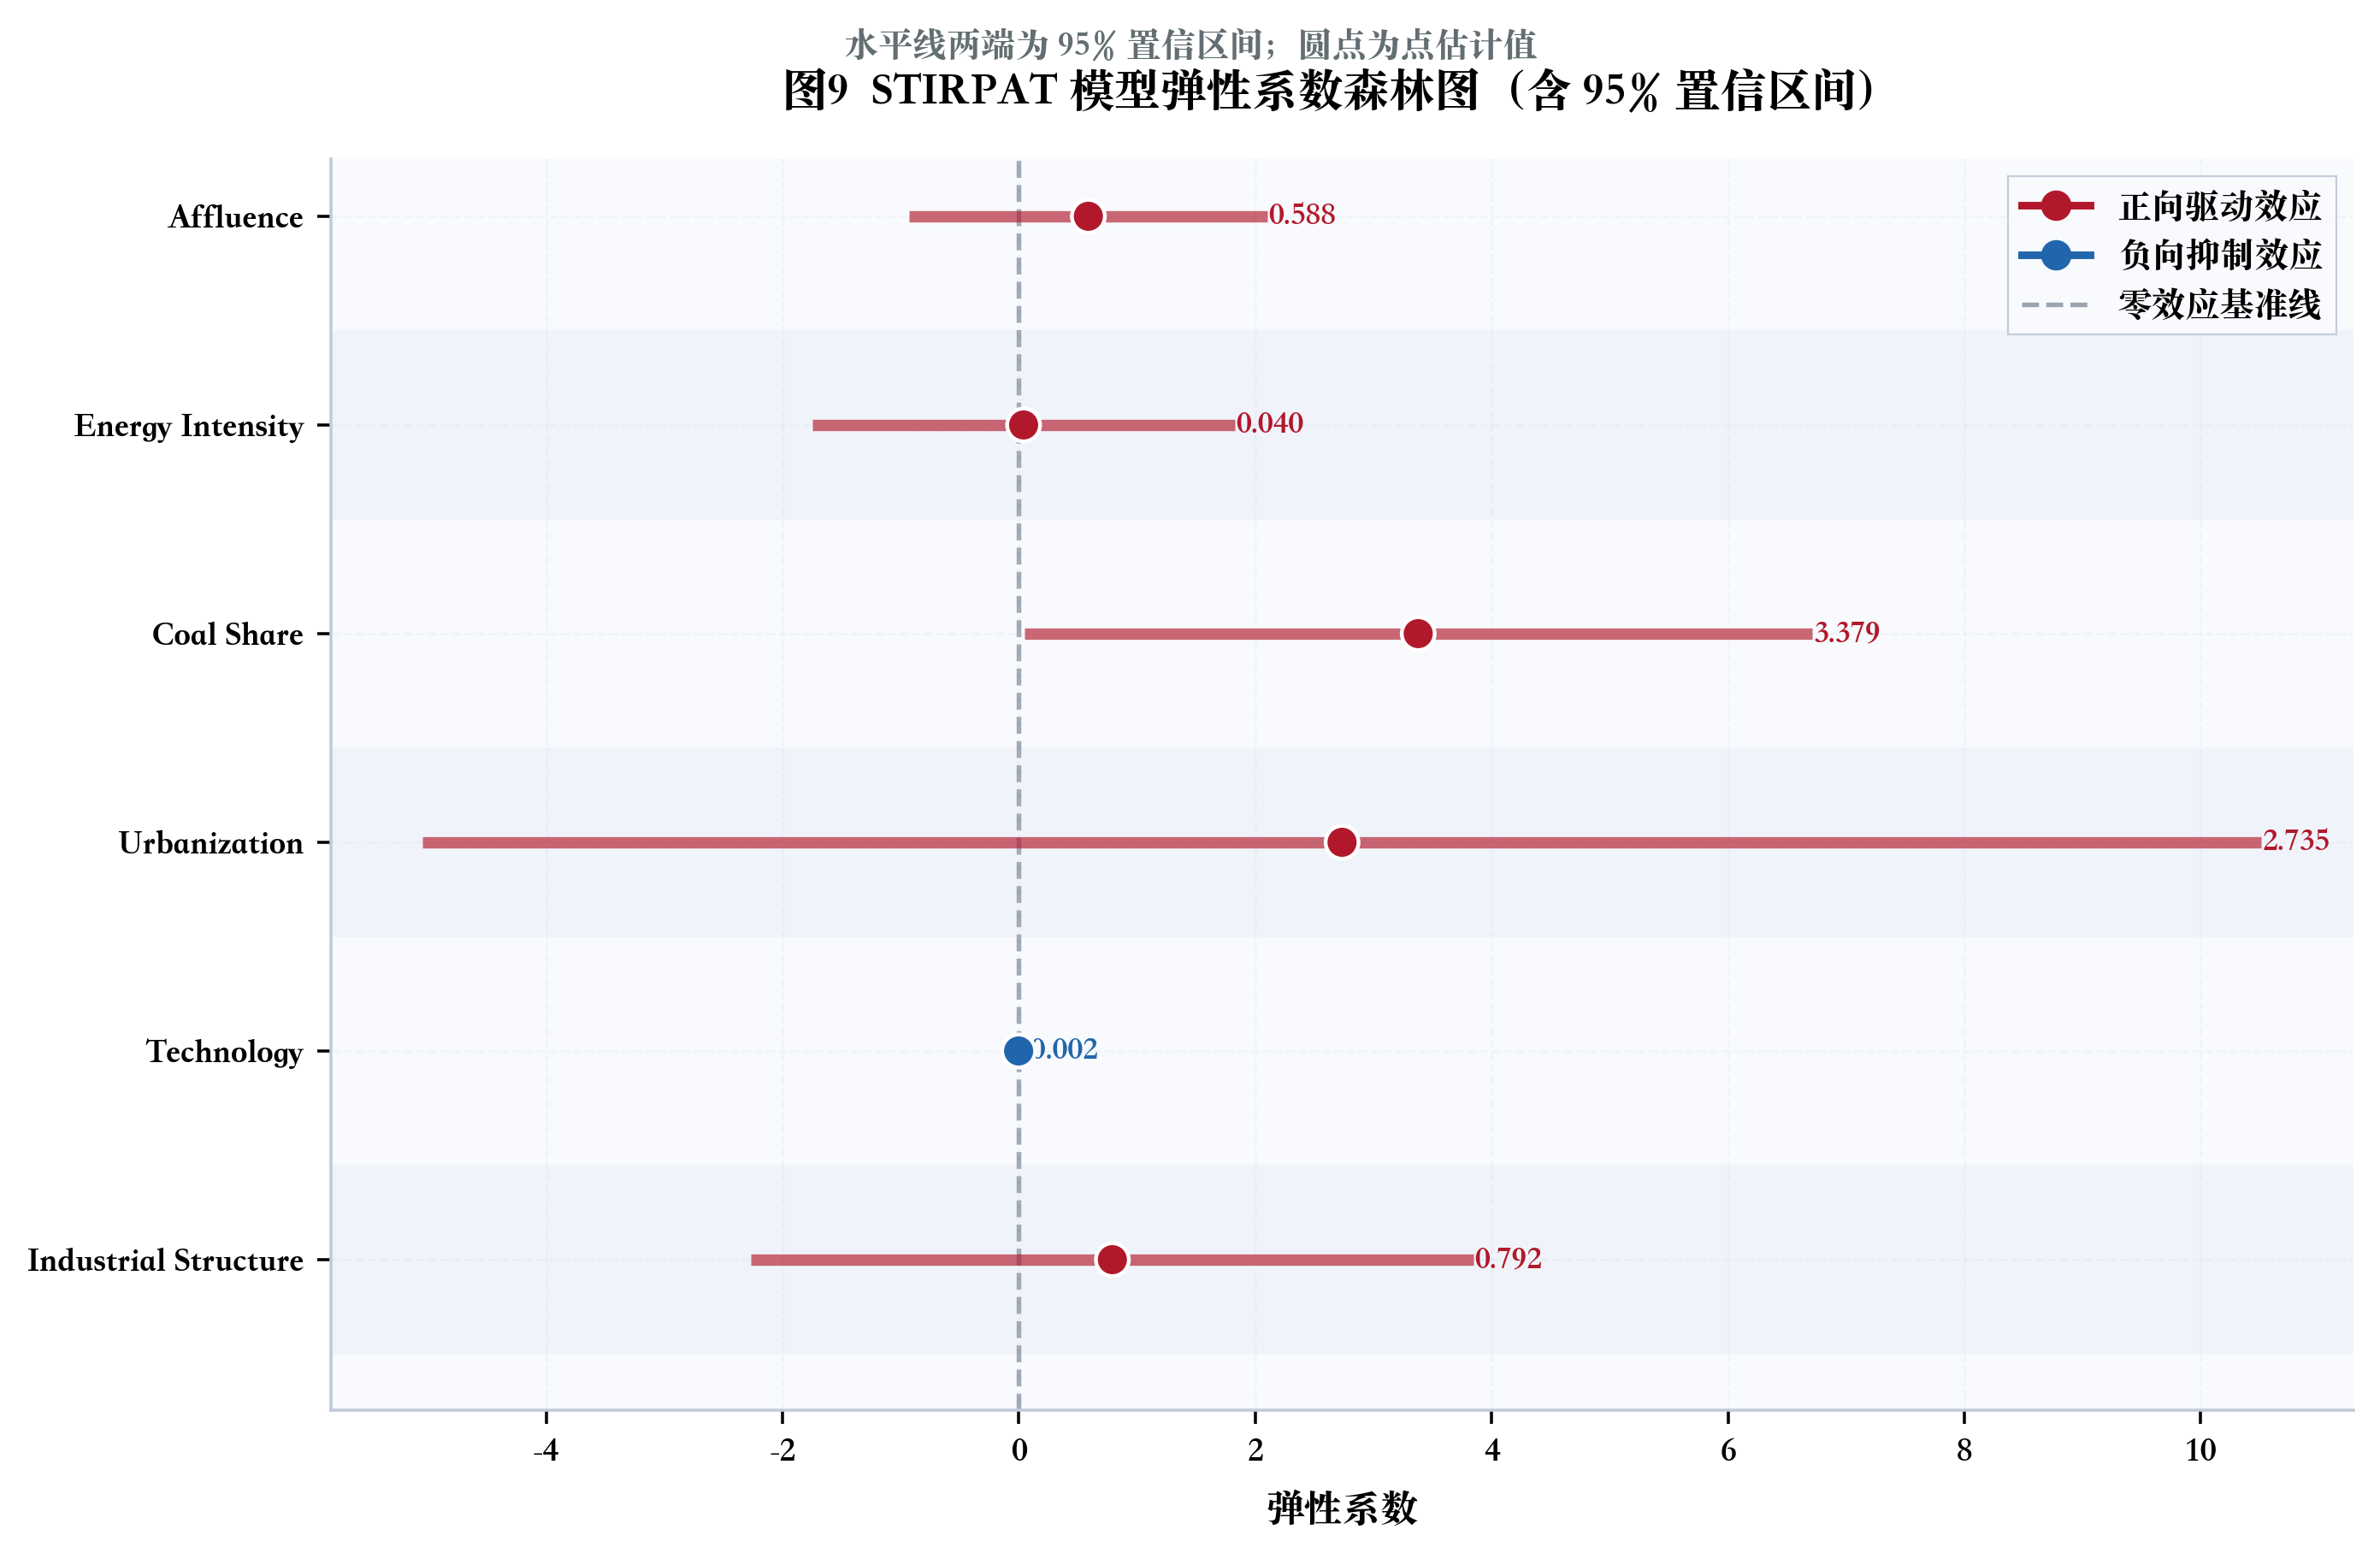
\includegraphics[width=0.78\textwidth]{../outputs/figures/Fig9_stirpat_coefficients.png}
    \captionof{figure}{扩展STIRPAT关键弹性系数图}
    \label{fig:stirpat}
\end{center}
图\ref{fig:stirpat}对应结果显示，在2005—2022年观测样本（18期）下，扩展STIRPAT回归需估计6个解释变量和截距项，共7个参数，自由度仅约11。受限于样本长度与小样本估计不确定性，系数区间普遍较宽。结果表明，仅煤炭占比在95\%置信水平下保持显著正向影响（弹性约3.3791，95\%置信区间[0.0469,\,6.7112]），是统计上最稳健的驱动因子；人均GDP、能源强度、城镇化和产业结构等变量虽点估计多为正，但置信区间包含零，未达到统计显著。这说明小样本条件下难以稳定识别其边际效应强度，但并不否定其经济机制上的现实作用，后续需通过延长样本期或进一步精简变量提高识别精度。

\begin{center}
    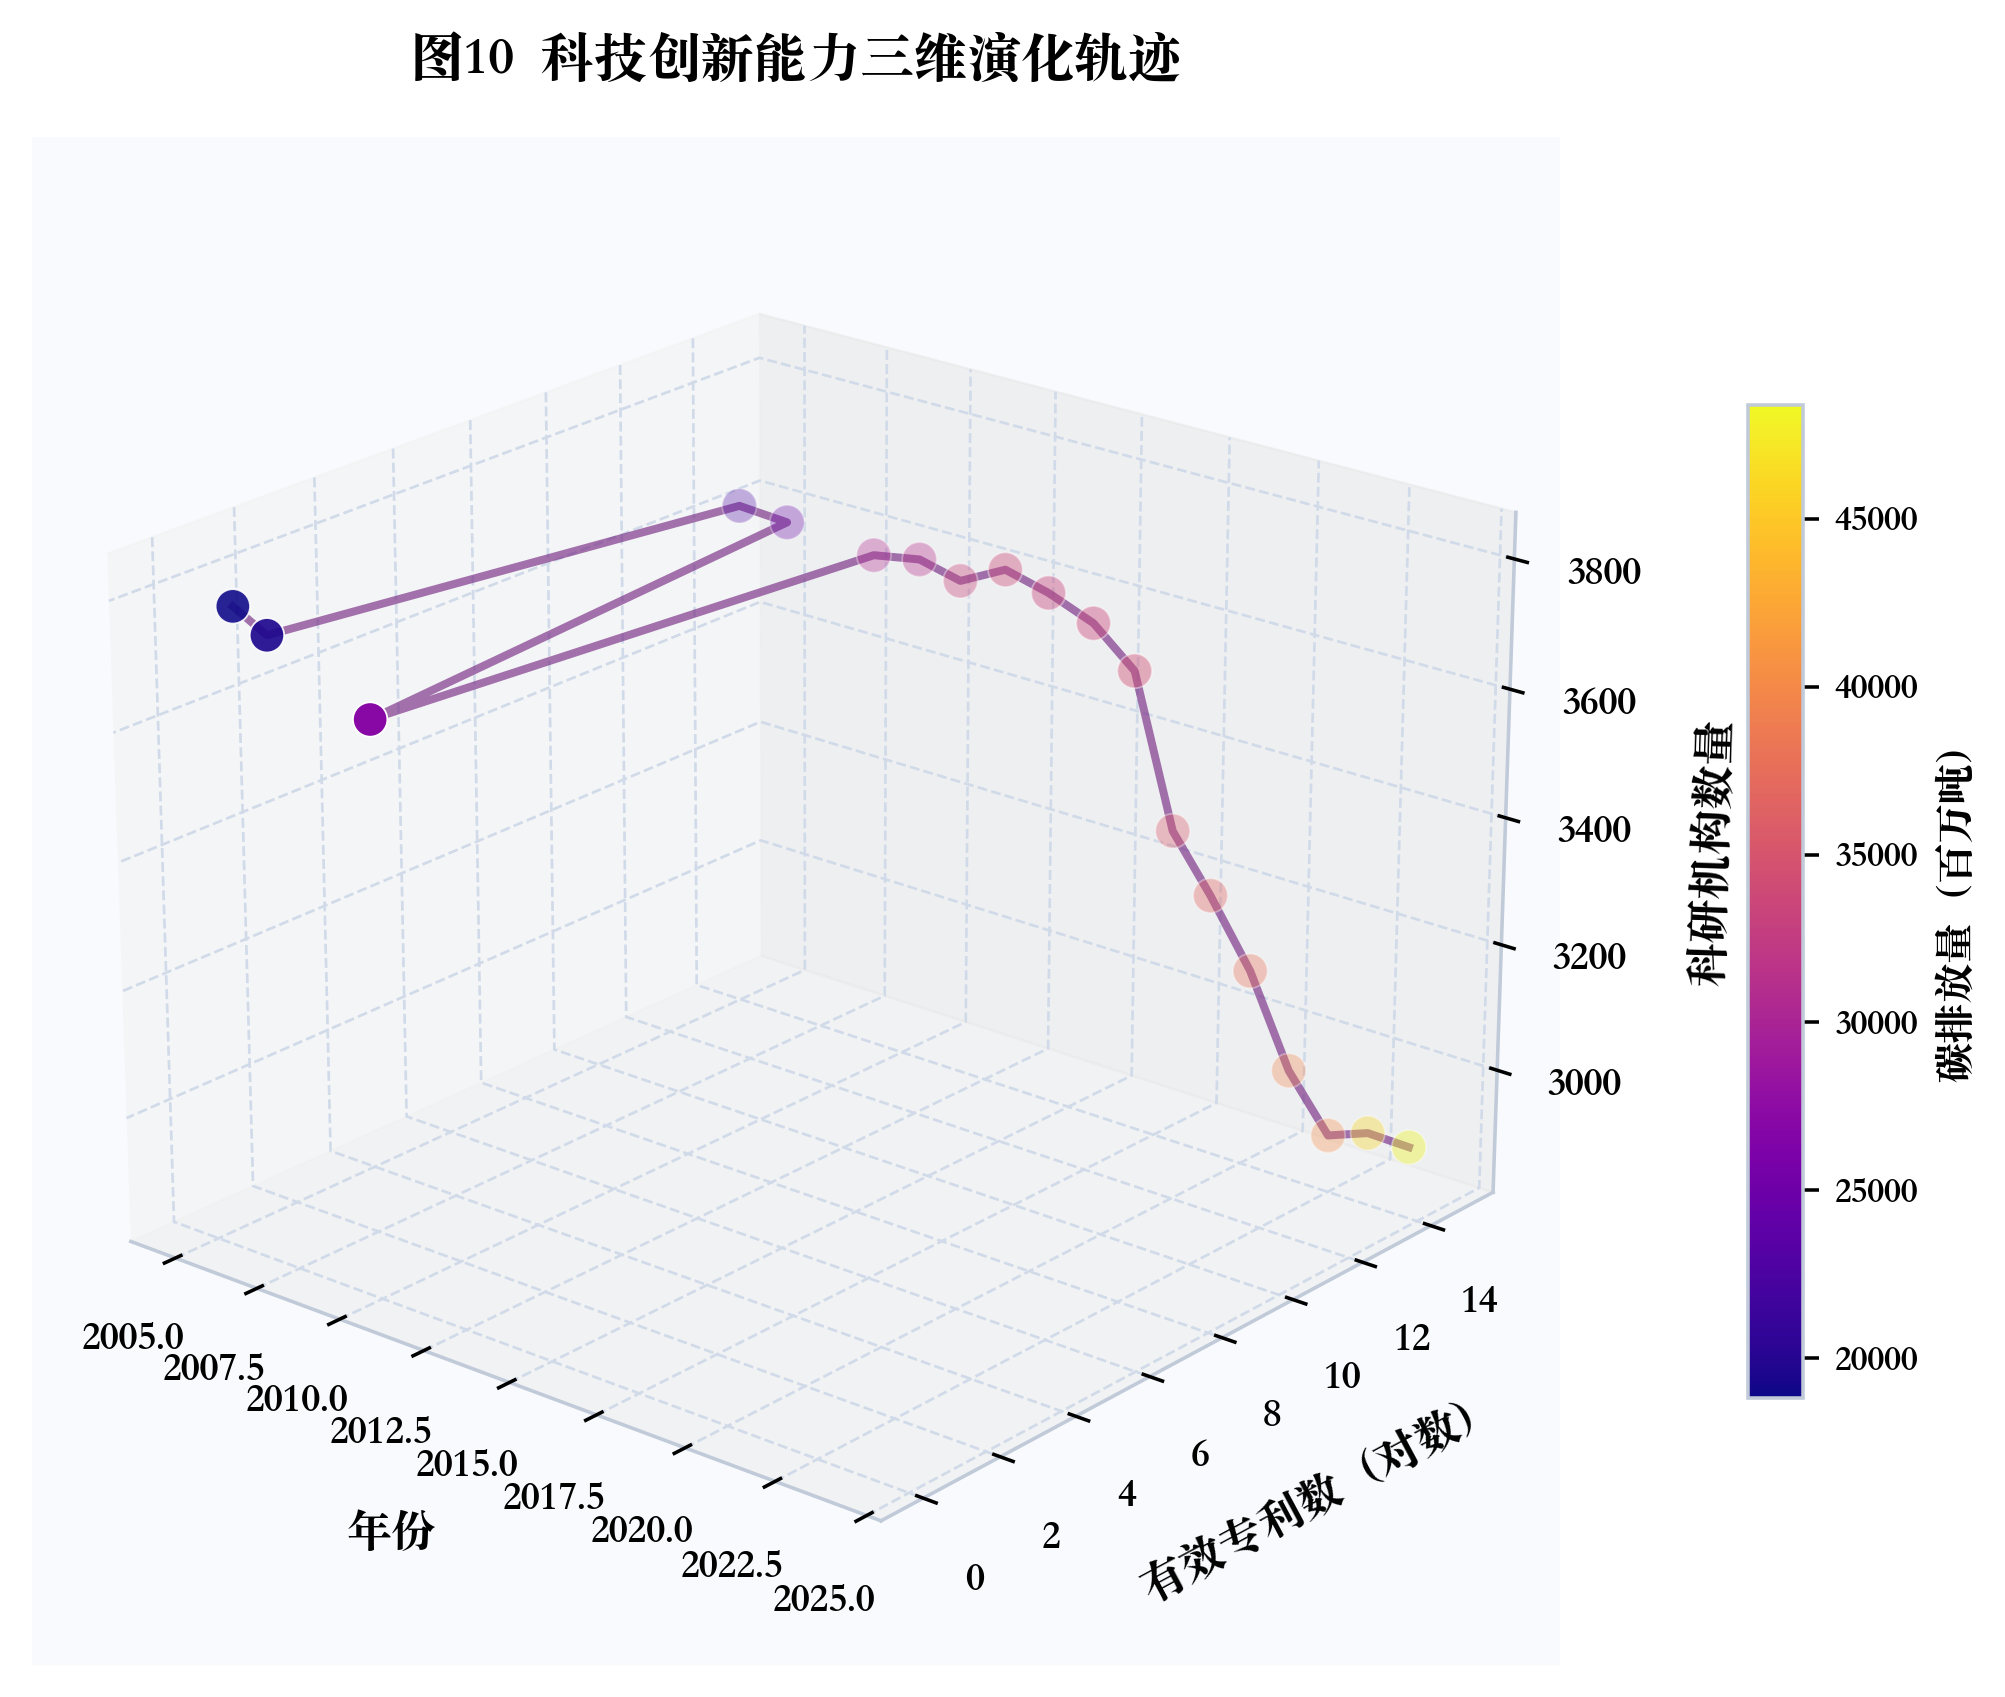
\includegraphics[width=0.78\textwidth]{../outputs/figures/Fig10_innovation_capacity.png}
    \captionof{figure}{技术创新能力三维轨迹图}
    \label{fig:innovation_3d}
\end{center}
从图\ref{fig:innovation_3d}可见，专利、科研机构与碳排放的三维轨迹更接近“缓释效应”特征，即技术因素通过时间积累逐步改变边际排放，而非在短期内直接逆转总量趋势。

\begin{table}[H]
\centering
\caption{扩展STIRPAT主要弹性系数估计结果}
\label{tab:stirpat_coeff}
\begin{tabular}{cccc}
\midrule
Affluence & 0.5882 & -0.9264 & 2.1027 \\
Energy Intensity & 0.0401 & -1.7464 & 1.8266 \\
Coal Share & 3.3791 & 0.0469 & 6.7112 \\
Urbanization & 2.7347 & -5.0452 & 10.5146 \\
Technology & -0.0018 & -0.0086 & 0.0049 \\
Industrial Structure & 0.7915 & -2.2662 & 3.8492 \\
\bottomrule
\end{tabular}
\end{table}

\subsection{预测与情景模拟}
本节聚焦两个问题：在小样本国家级时序中何种模型更稳健，以及不同政策强度下峰值水平可被压低到何种区间。

\begin{center}
    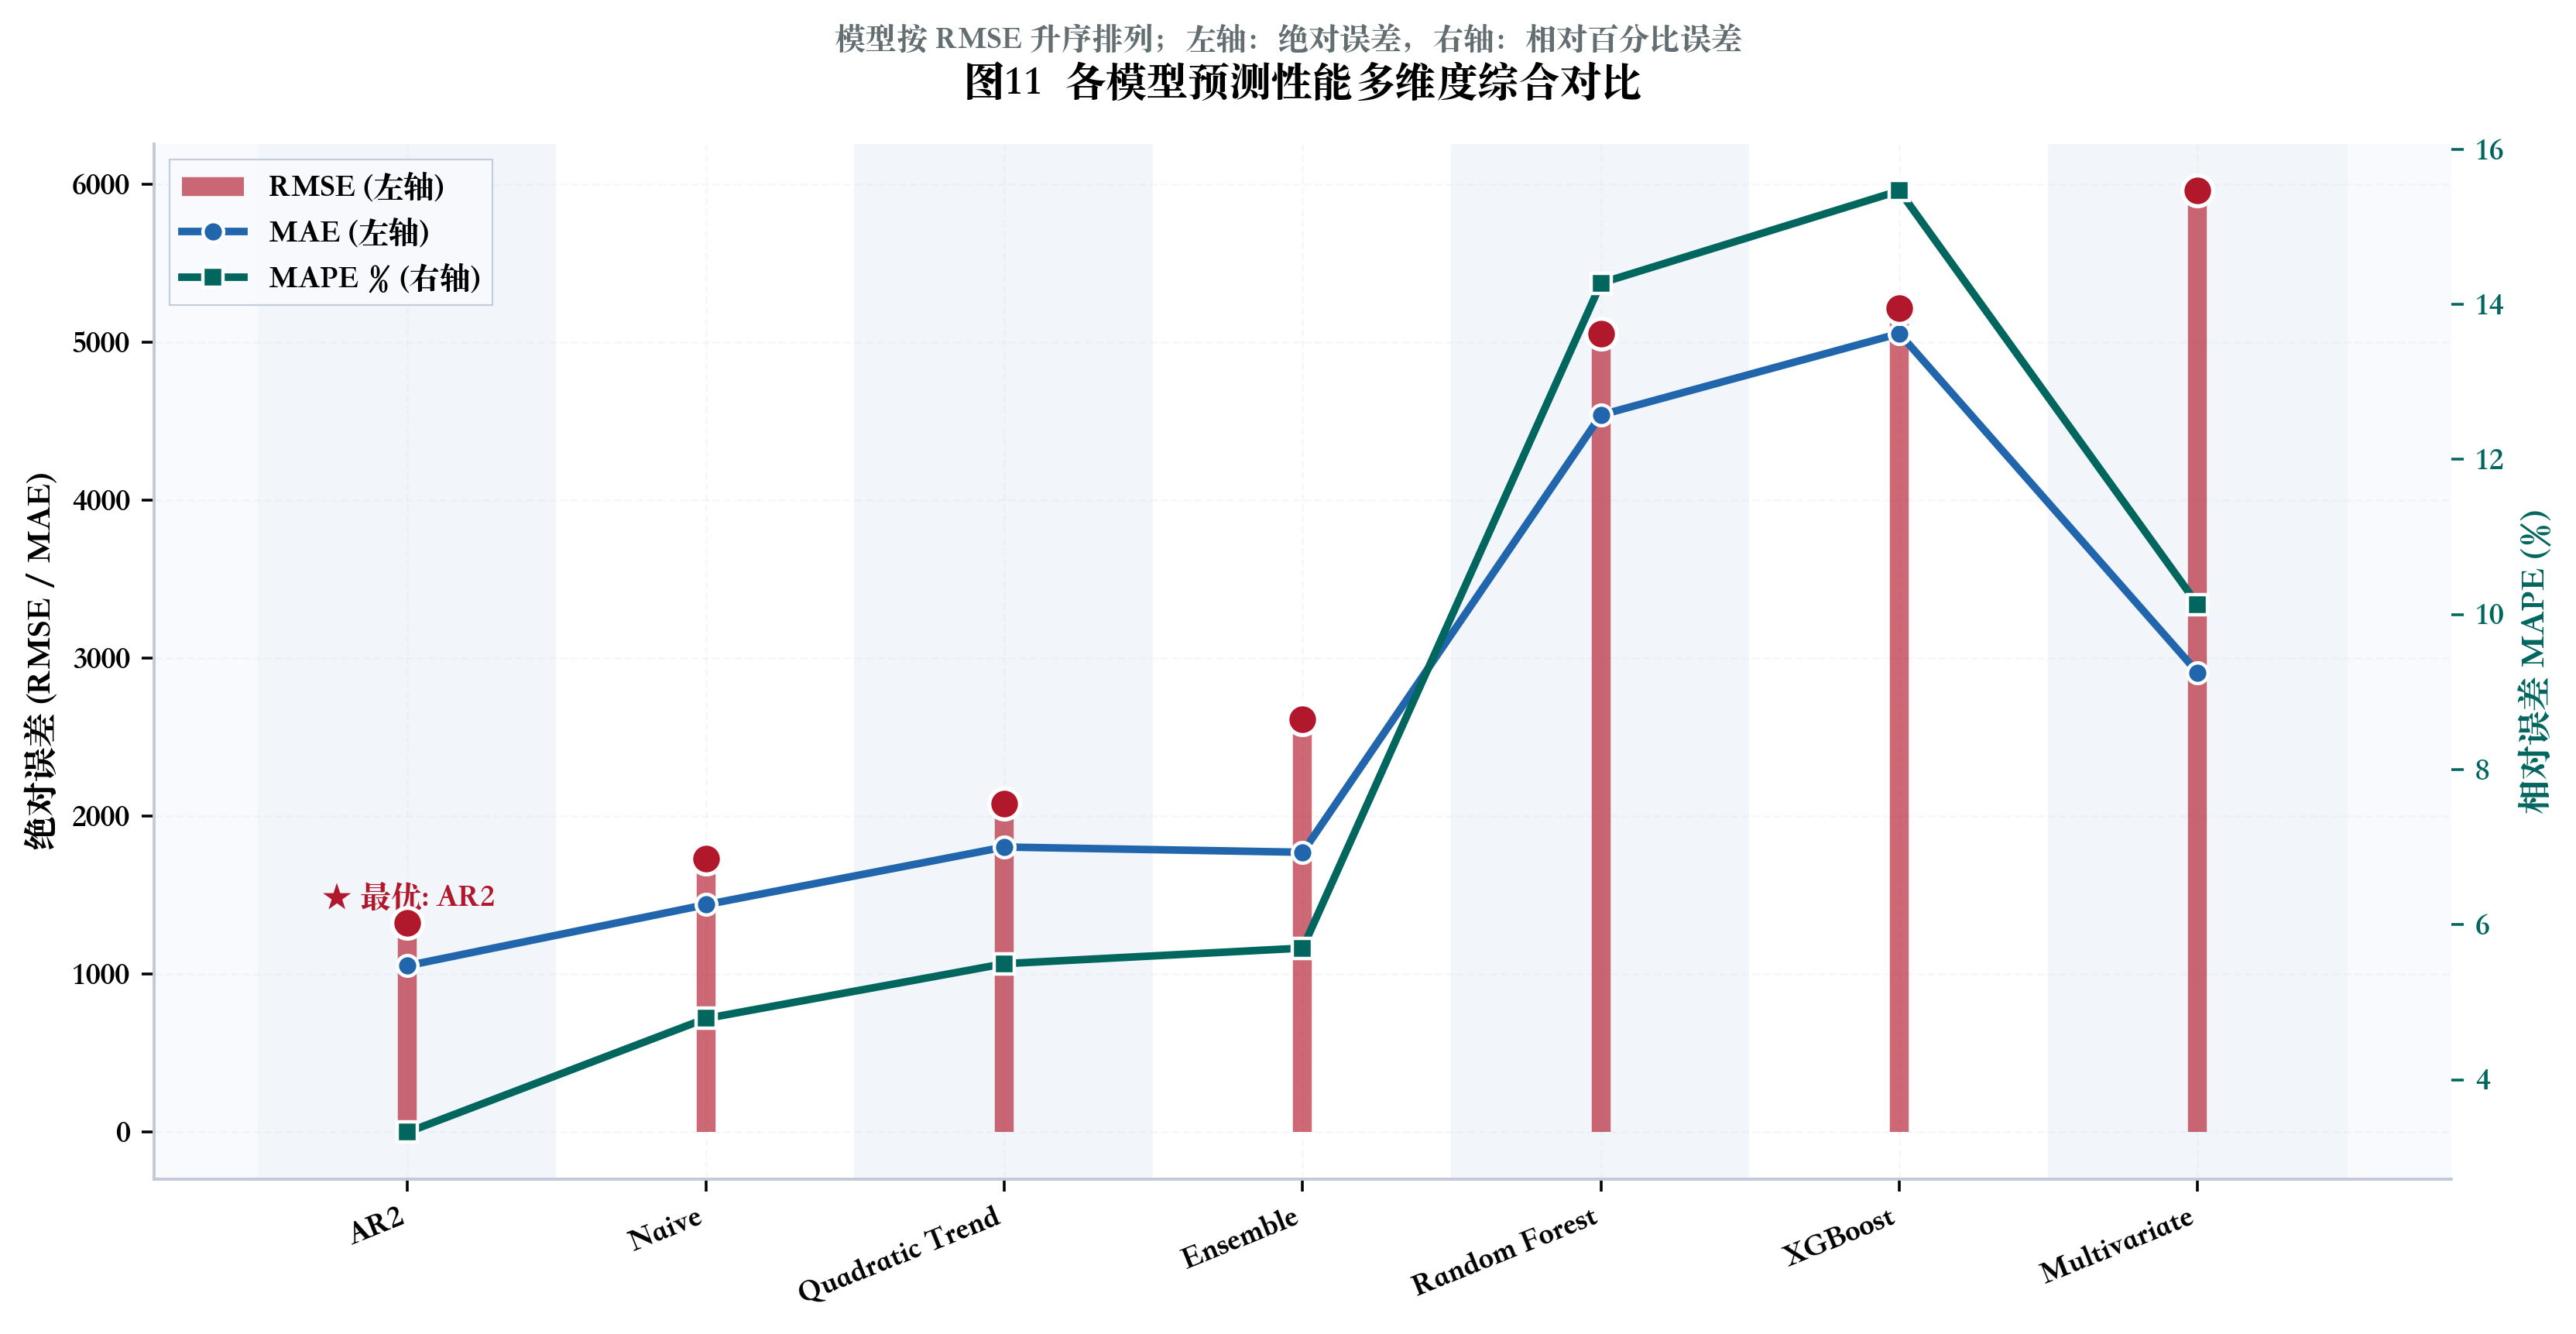
\includegraphics[width=0.80\textwidth]{../outputs/figures/Fig11_model_performance.png}
    \captionof{figure}{多模型滚动预测误差比较}
    \label{fig:model_perf}
\end{center}
图\ref{fig:model_perf}显示，在统一可比窗口下，AR2 模型误差最低（RMSE=1323.36，MAPE=3.32\%），朴素模型次之；二次趋势模型表现尚可。然而，值得关注的现象是，引入高维特征或多树集成的复杂模型出现了显著的性能崩塌：XGBoost（RMSE=5214.83）与随机森林（RMSE=5054.08）的误差远高于传统基准，多变量回归也表现不佳。这一“复杂度失效”现象并非算法本身的缺陷，而是由国家级时序样本量极小（仅18期观测值）导致的严重过拟合——树模型无法在极少样本中提取稳健的分裂规则，导致外推方差急剧放大。该结果以直观的对比形式，有力地支撑了本文“模型适配性优先于模型复杂度”的核心论断。

单位根检验表明序列为 I(1) 过程，解释了为何依赖序列动态的 AR 模型更稳健，而水平拟合的高复杂度模型易累积误差。
\begin{center}
    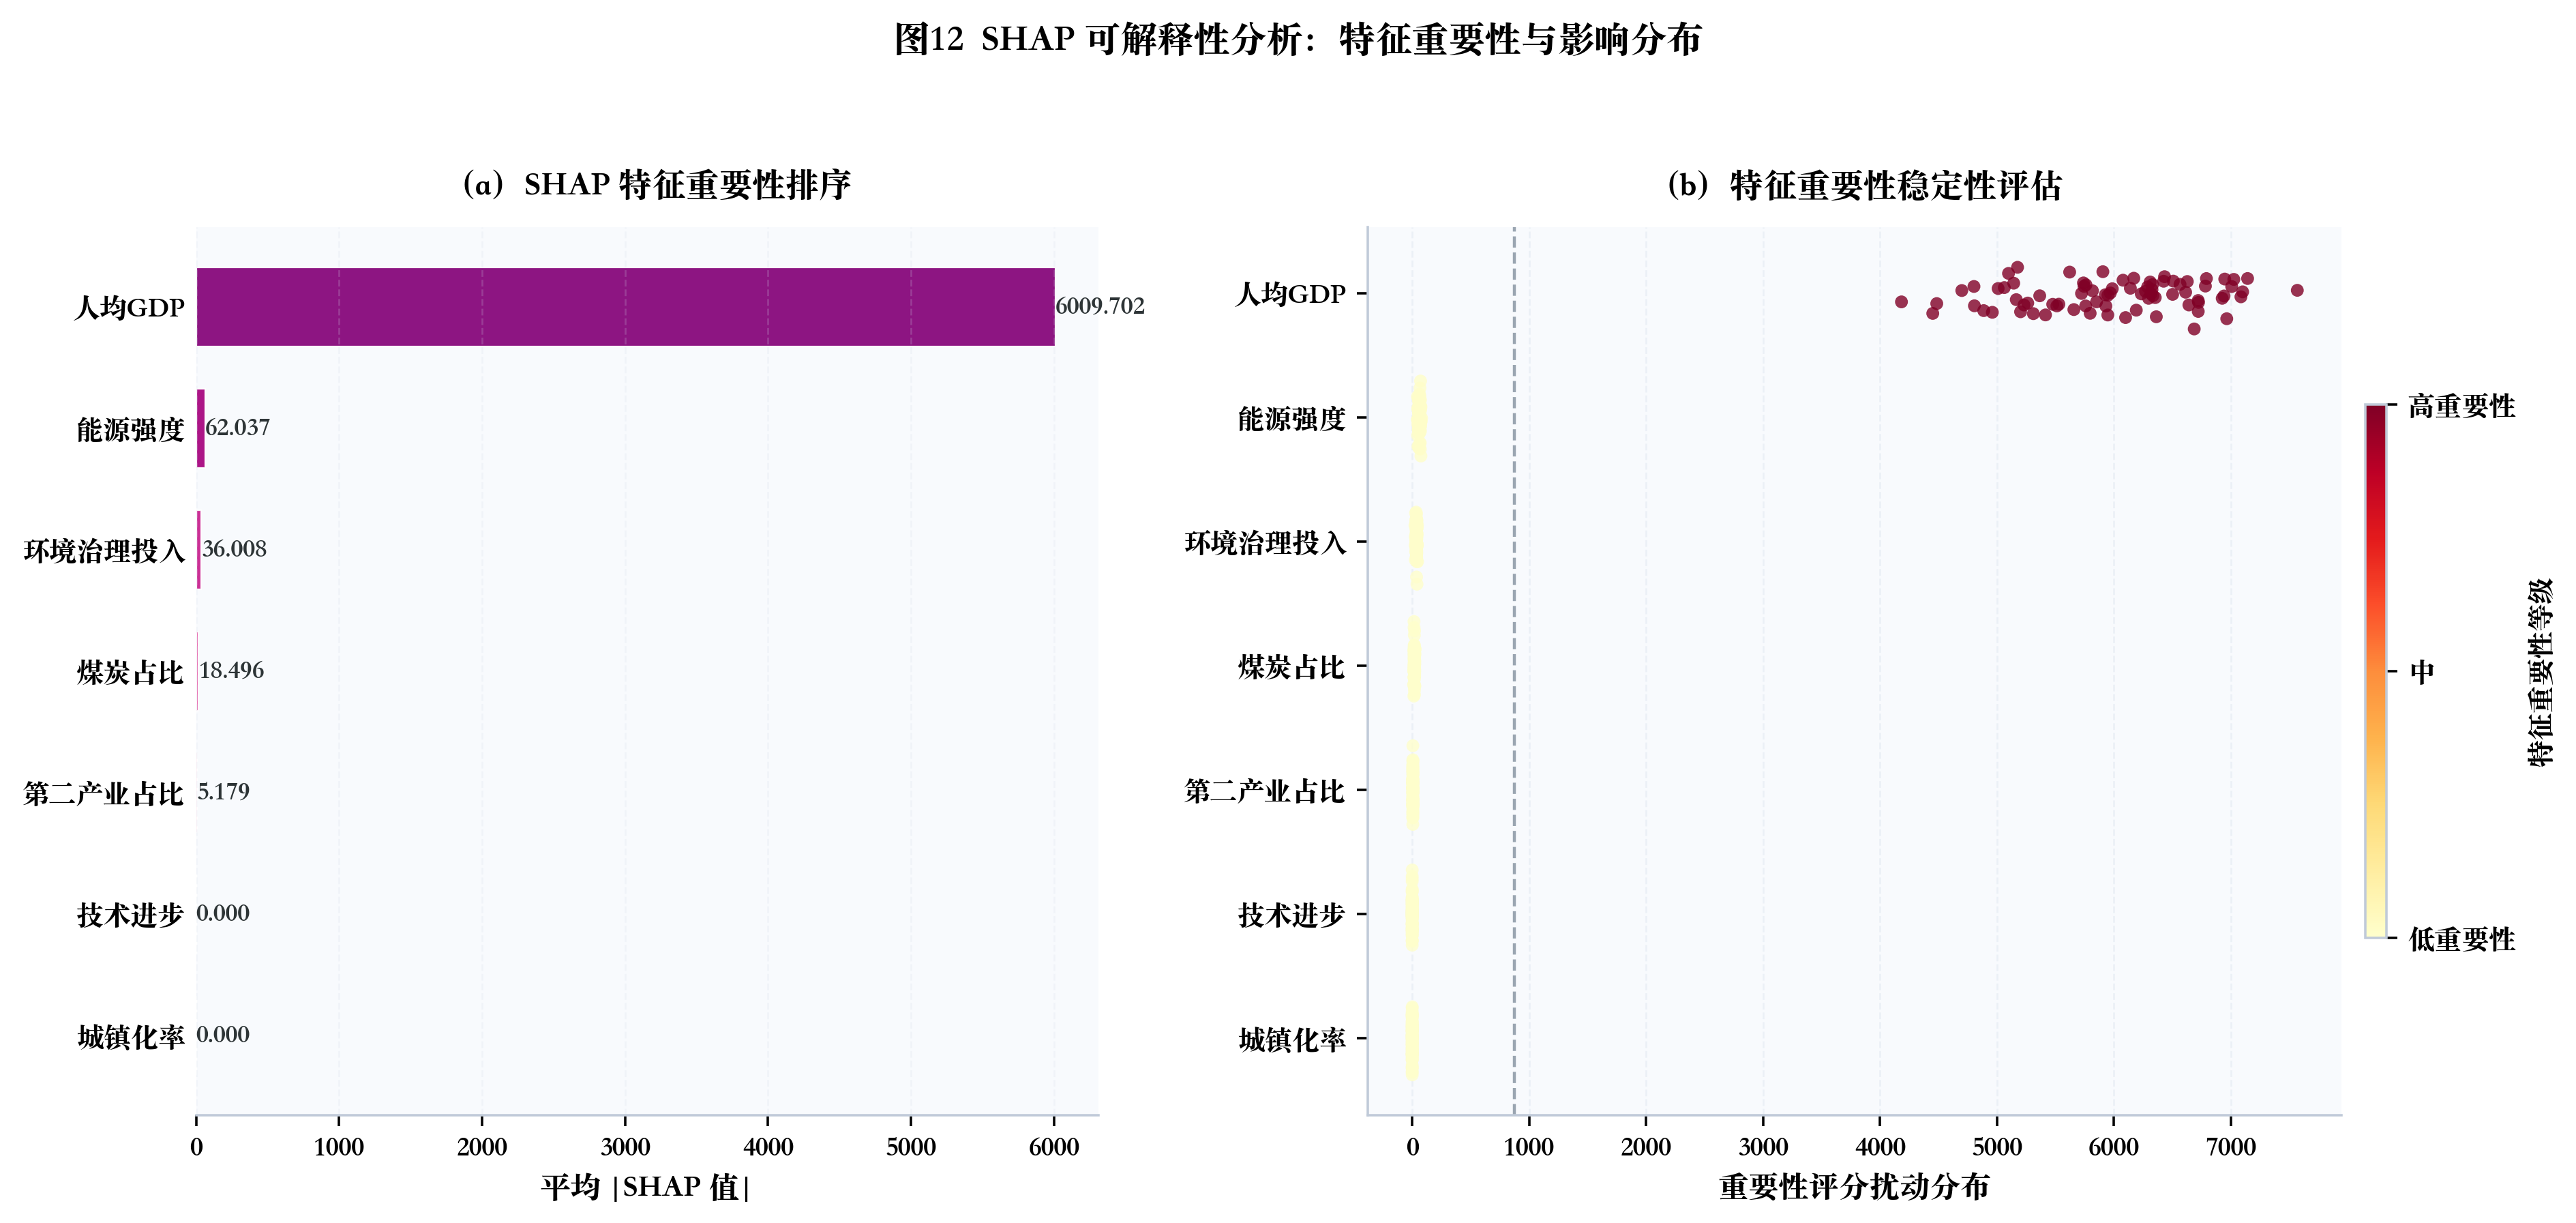
\includegraphics[width=0.92\textwidth]{../outputs/figures/Fig12_shap_summary.png}
    \captionof{figure}{基于XGBoost模型的特征重要性SHAP分析}
    \label{fig:shap}
\end{center}
图\ref{fig:shap}a）展示了基于 XGBoost 模型的真实 SHAP 全局特征重要性排序。结果显示，人均 GDP 的平均绝对 SHAP 值远超其他变量，呈现出明显的``主导地位''，而城镇化率与技术进步的特征重要性为 0。

这一结果看似与前文STIRPAT中“煤炭占比最显著”的结论相左，实则反映了小样本下复杂模型在特征选择上的局限性。具体而言，在仅有18期的宏观时序中，人均GDP与碳排放高度共线。XGBoost在节点分裂时，直接被该主导特征主导，导致其他变量的特征重要性被完全掩盖。

反观前文的 STIRPAT 模型，其本质是多元线性回归，强制要求所有变量在同一方程中竞争解释力（控制了共线性与规模效应）。正是这种机制，识别出了煤炭占比的独立正向弹性。此外，SHAP结果中城镇化与技术进步重要性为0，也与STIRPAT中二者未达统计显著的结果相互印证。

综合来看，SHAP分析从侧面证实了前文的判断：小样本下盲目追求算法复杂度，不仅损害预测外推性，还容易导致机制识别的失真。

\begin{table}[H]
\centering
\caption{主要模型预测误差比较}
\label{tab:model_perf}
\begin{tabular}{cccc}
\toprule
模型 & RMSE & MAE & MAPE(\%) \\
\midrule
AR2 & 1323.36 & 1054.50 & 3.32 \\
Naive & 1732.09 & 1440.44 & 4.79 \\
Quadratic Trend & 2081.10 & 1805.35 & 5.50 \\
Ensemble & 2612.10 & 1772.16 & 5.70 \\
Random Forest & 5054.08 & 4540.33 & 14.27 \\
XGBoost & 5214.83 & 5056.28 & 15.47 \\
Multivariate & 5959.72 & 2909.50 & 10.13 \\
\bottomrule
\end{tabular}
\end{table}

\begin{center}
    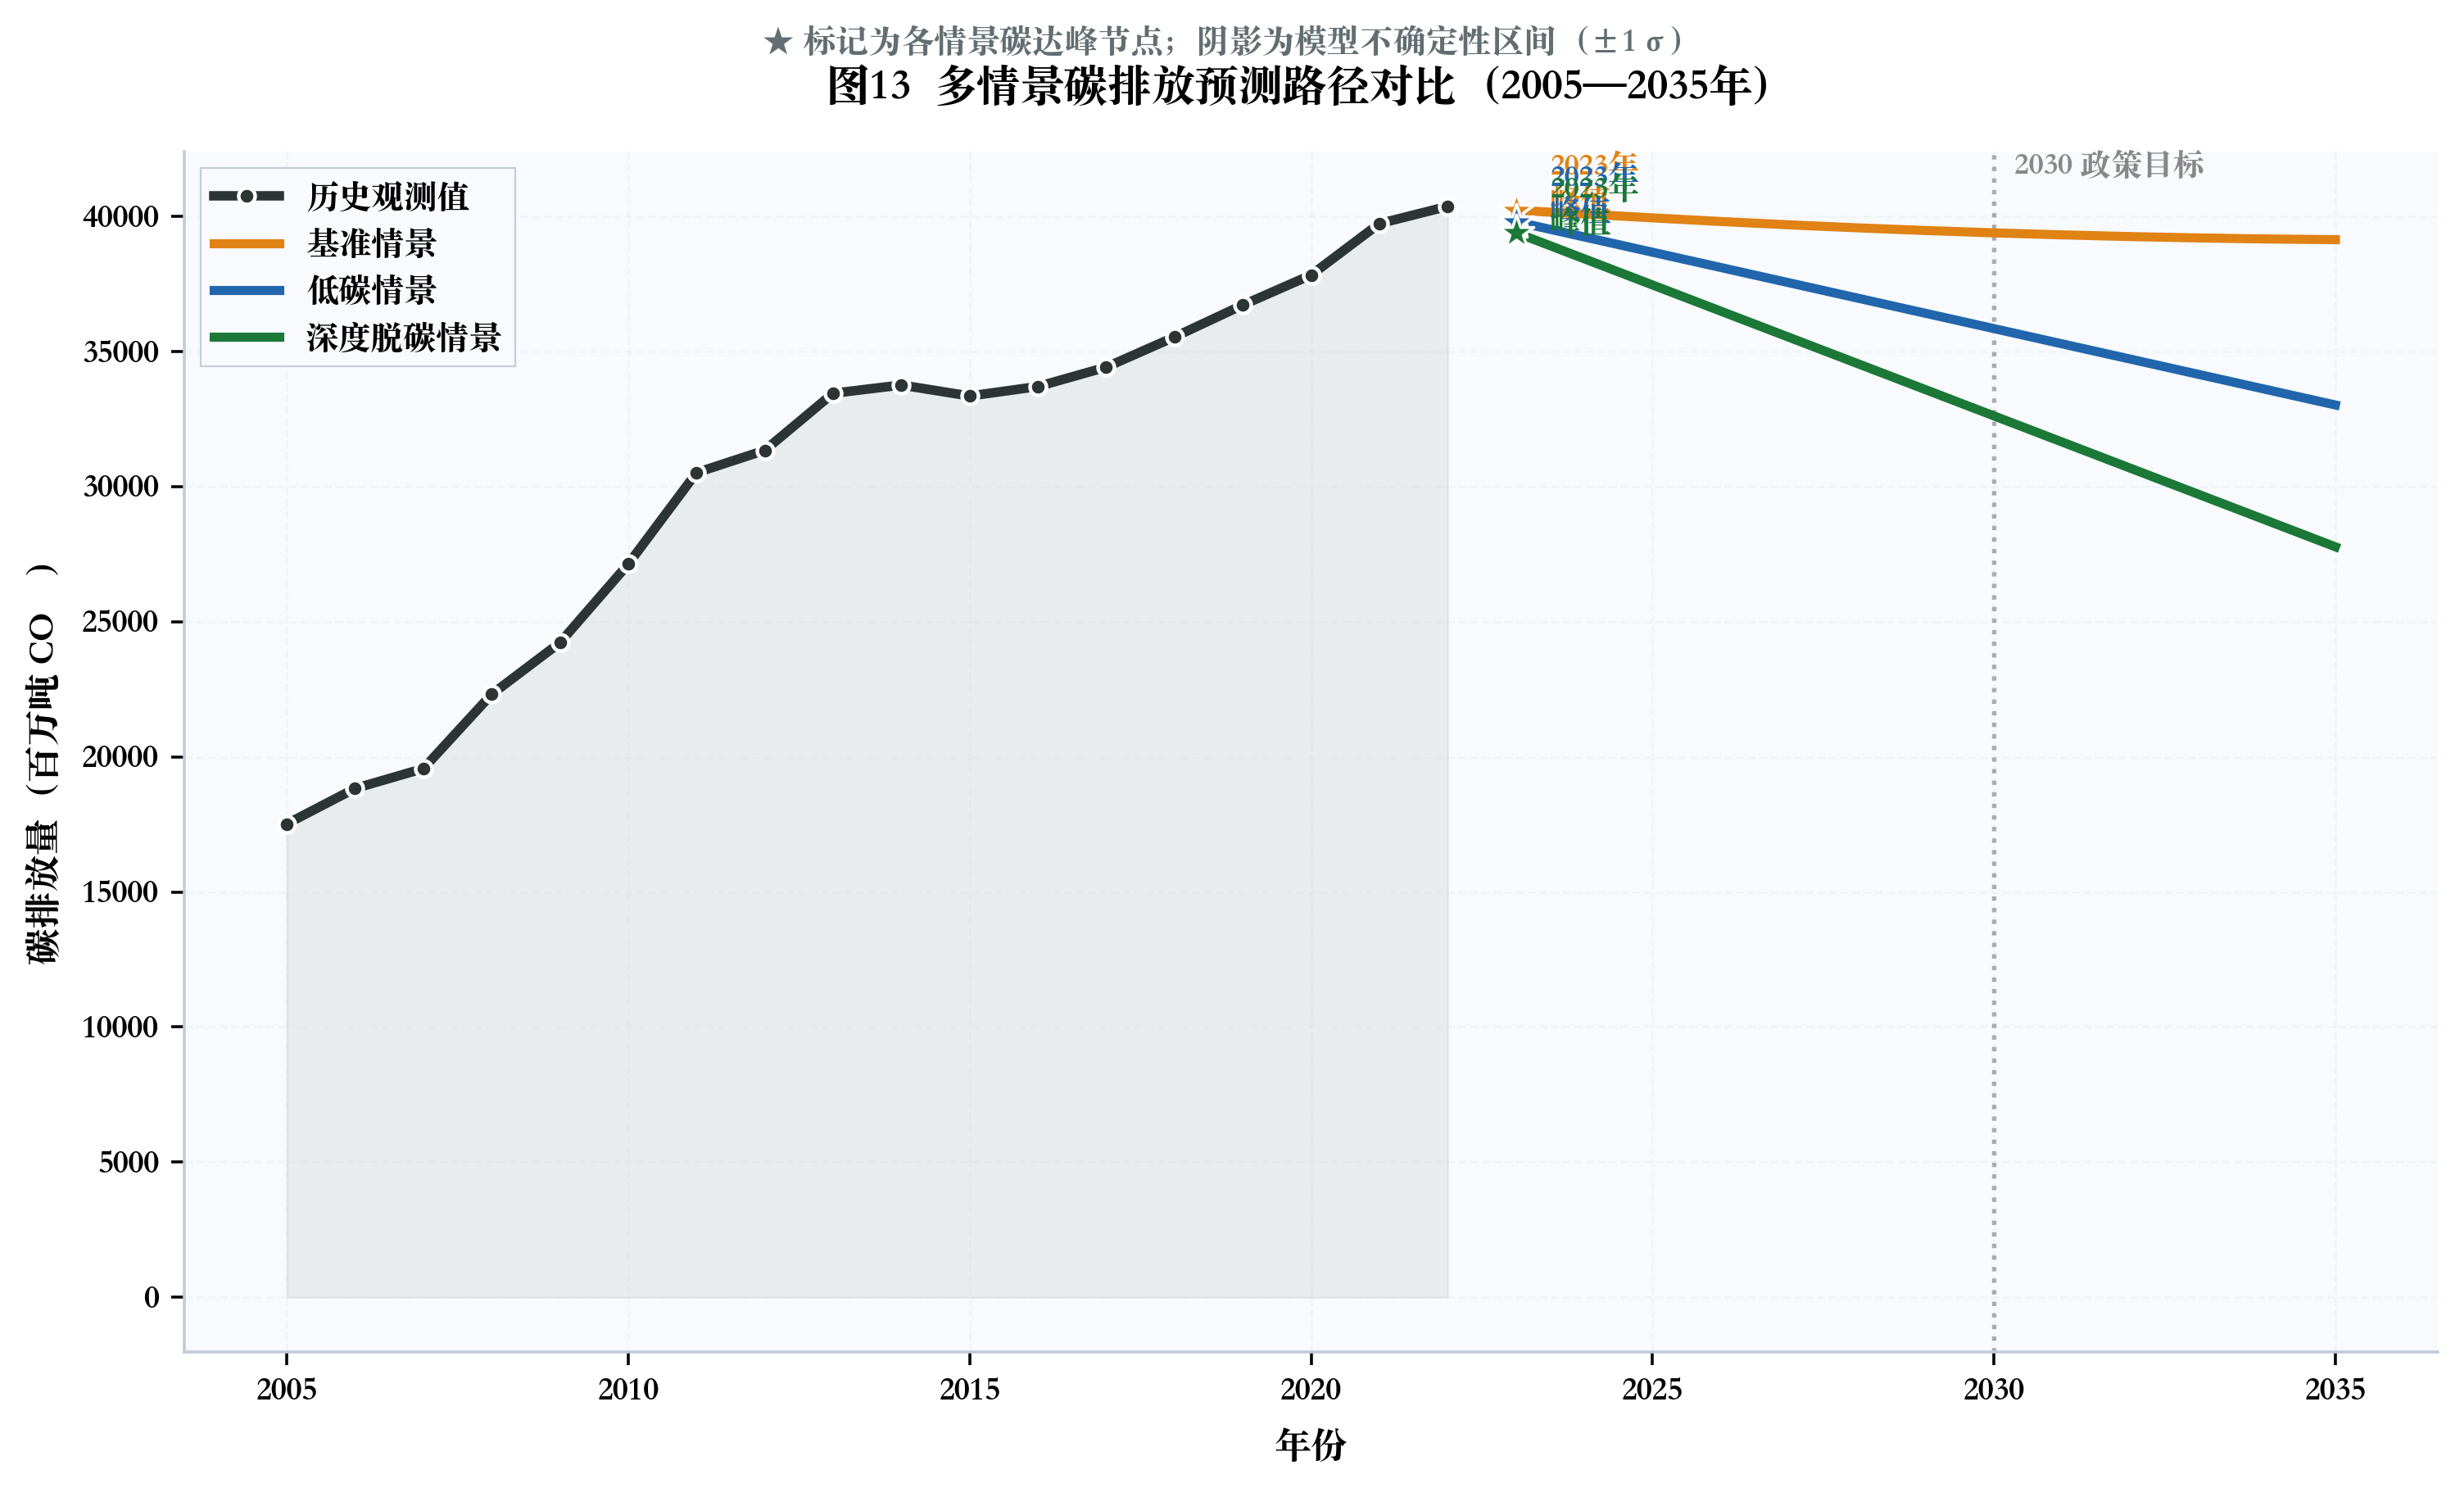
\includegraphics[width=0.82\textwidth]{../outputs/figures/Fig13_scenario_paths.png}
    \captionof{figure}{不同情景下碳排放路径预测比较（2025—2035）}
    \label{fig:scenario_paths}
\end{center}
从图\ref{fig:scenario_paths}可以看到，基准、低碳和深度脱碳三类情景在2025—2035年形成明显分叉。到2035年，基准约39127.33 Mt，低碳约33013.06 Mt，深度脱碳约27766.48 Mt。

\begin{center}
    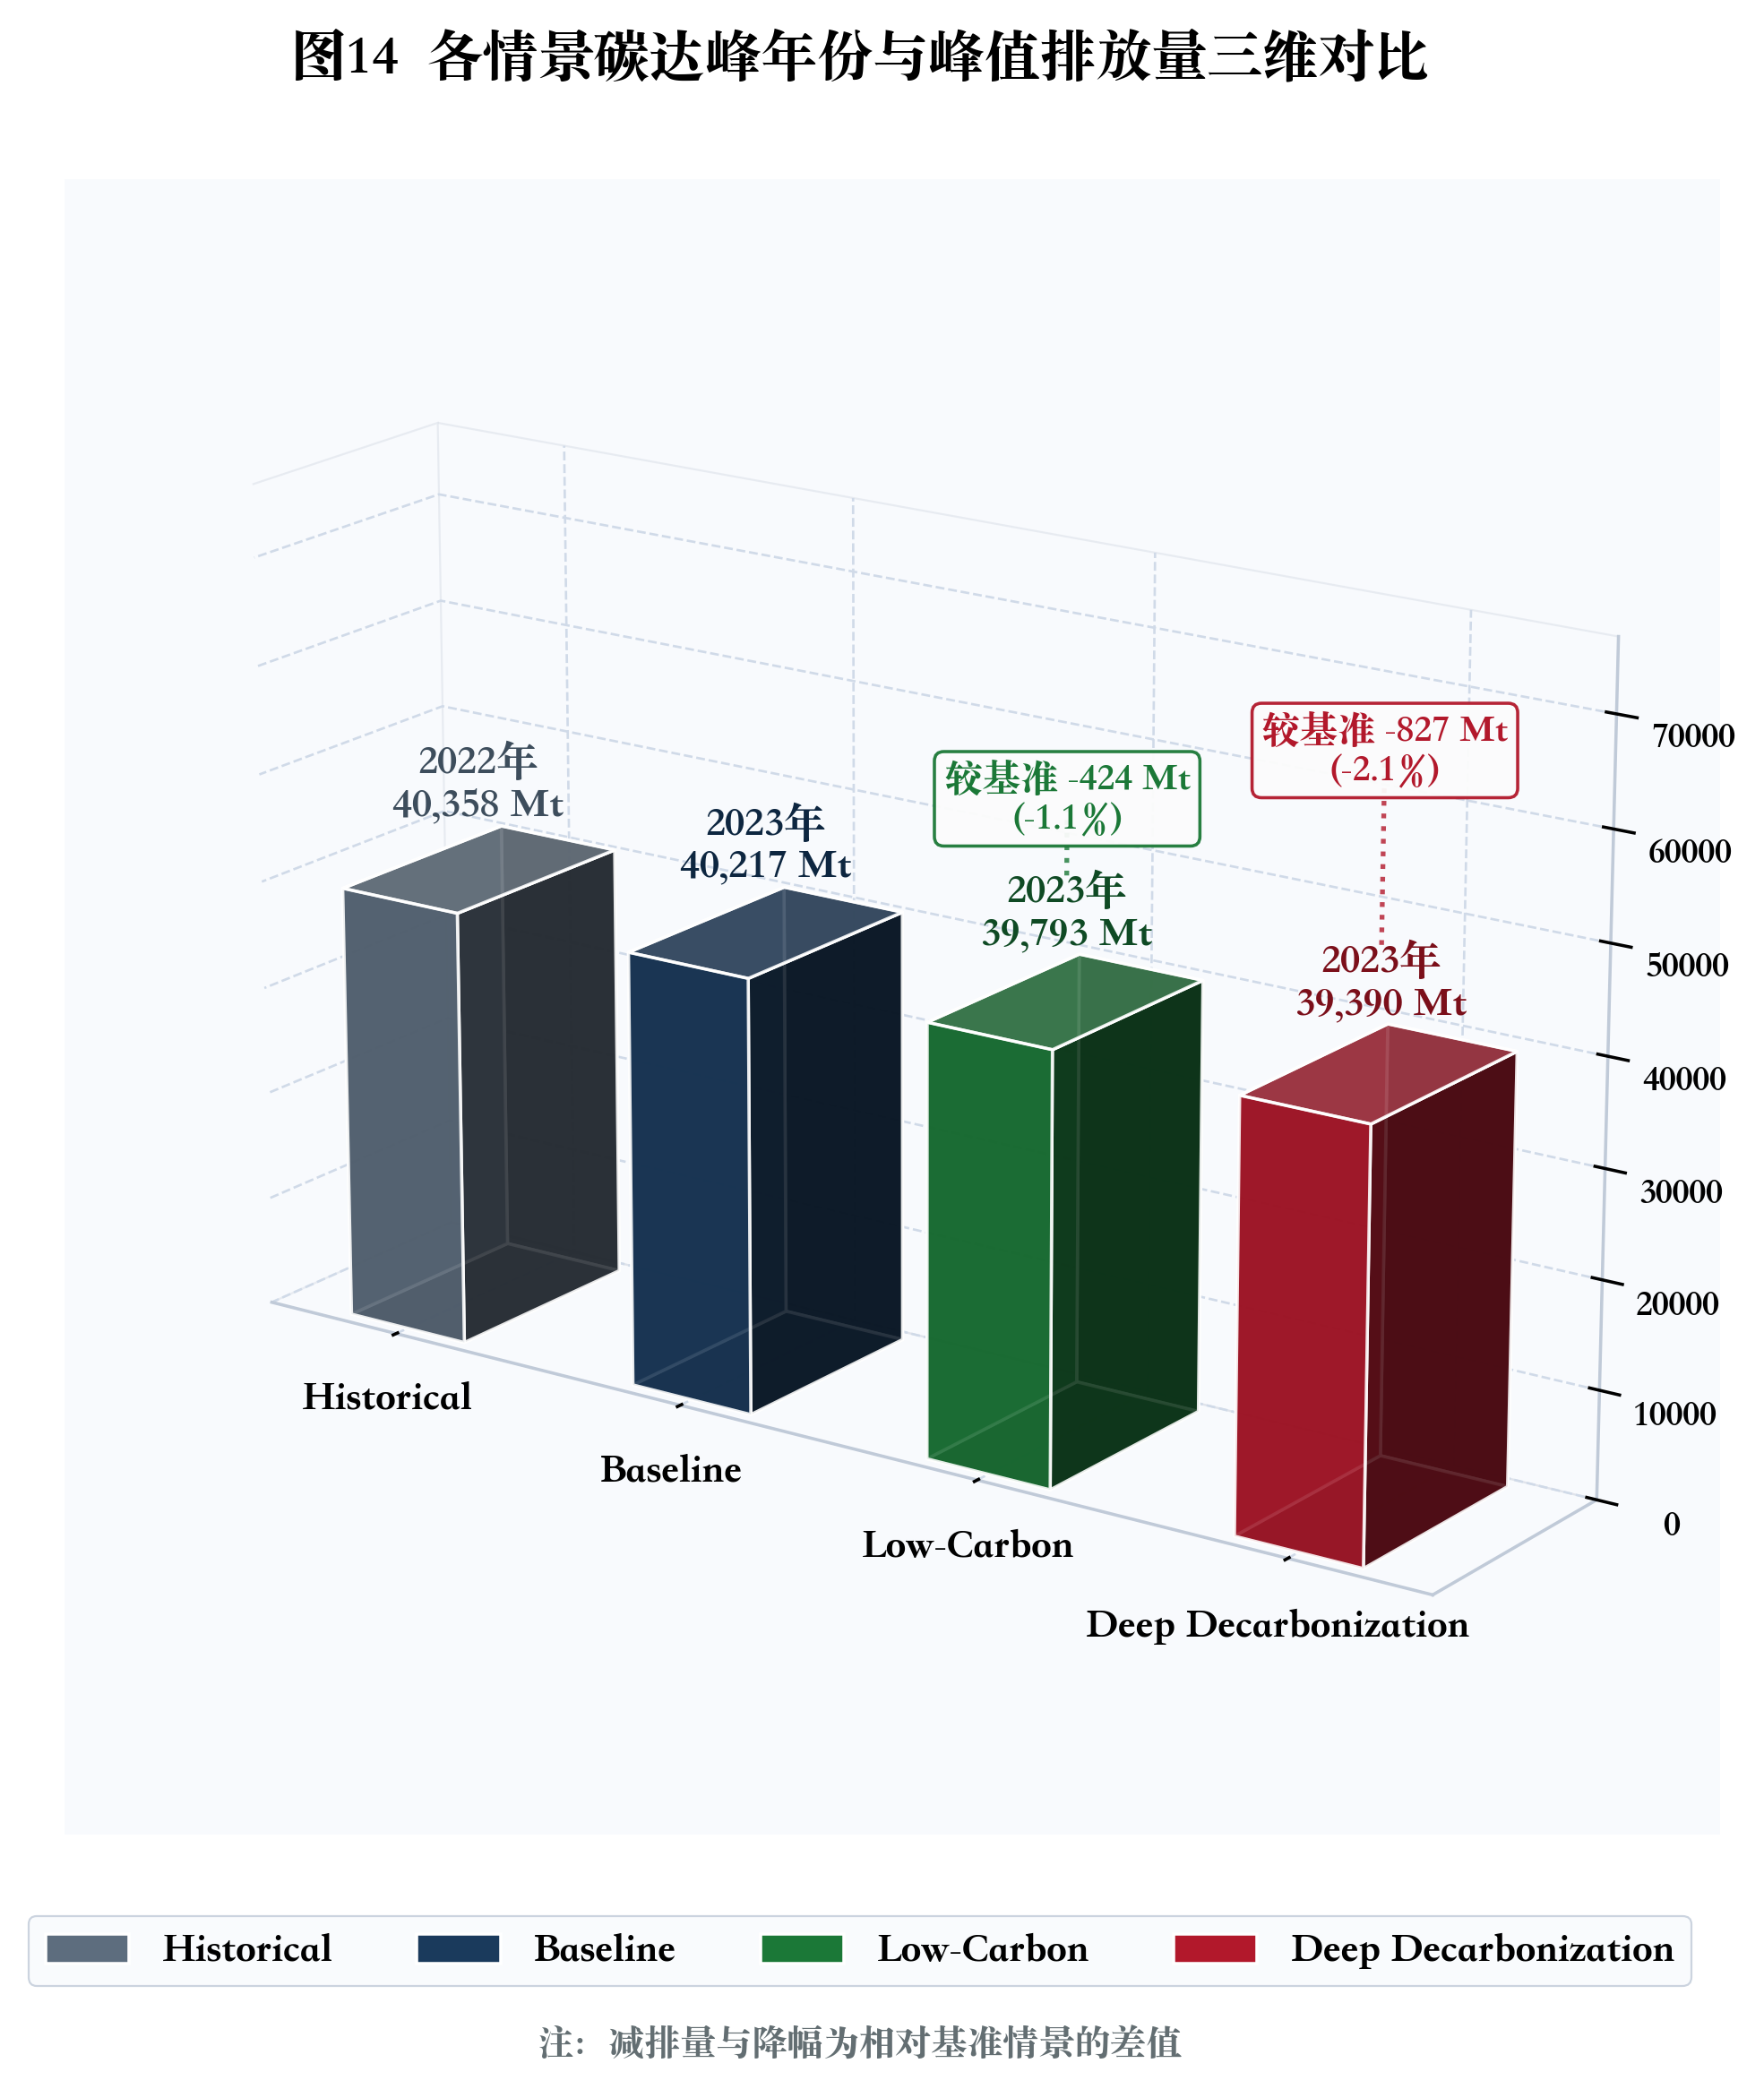
\includegraphics[width=0.80\textwidth]{../outputs/figures/Fig14_peak_bubble.png}
    \captionof{figure}{不同情景峰值年份与峰值规模三维比较}
    \label{fig:peak_3d}
\end{center}
图\ref{fig:peak_3d}显示，历史观测路径峰值约40358.26 Mt（2022年），三类政策情景下峰值均低于该历史高点。

\begin{table}[H]
\centering
\caption{多情景核心参数设定表}
\label{tab:scenario_params}
\small 
\begin{tabularx}{\textwidth}{lXXX} 
\toprule
情景 & GDP年均增速(\%) & 煤炭占比年均变动(百分点) & 能源强度年均下降(\%) \\
\midrule
Baseline & 5.0 & -0.6 & 2.3 \\
Low-Carbon & 4.6 & -1.1 & 2.8 \\
Deep Decarbonization & 4.4 & -1.6 & 3.6 \\
\bottomrule
\end{tabularx}

{\footnotesize 注：参数区间参考《“十四五”现代能源体系规划》与国家统计局近年宏观运行区间设定。}
\end{table}

\begin{table}[H]
\centering
\caption{2035年不同情景碳排放预测结果}
\label{tab:scenario_2035}
\begin{tabular}{cc}
\toprule
情景 & 2035年碳排放(Mt) \\
\midrule
Baseline & 39127.33 \\
Low-Carbon & 33013.06 \\
Deep Decarbonization & 27766.48 \\
\bottomrule
\end{tabular}
\end{table}

表\ref{tab:scenario_params}给出了三类情景的参数设定。参数锚定于国家能源结构优化与能效提升目标导向，并结合近年宏观运行区间设定，用于构造可比的政策强度梯度。表\ref{tab:scenario_2035}与图\ref{fig:scenario_paths}、图\ref{fig:peak_3d}相互印证：在能源替代、产业升级、技术扩散三方面同步加力，可将未来峰值压至更低平台，进而降低长期减排成本。

\section{结果讨论与政策含义}
\subsection{结果讨论}
结合实证章节结果可以看出，我国碳排放变化并非由单一变量决定，而是规模因素与结构因素共同作用的结果。扩展STIRPAT估计显示，在2005—2022年小样本条件下，仅煤炭占比在95\%置信水平下保持显著正向影响，是统计上最稳健的驱动因子。人均GDP、能源强度、城镇化率与第二产业比重等变量点估计方向虽与经济直觉一致，但区间较宽且跨越零，提示其作用强度识别仍受自由度约束。

与此同时，城镇化率与技术进步变量的估计结果并不稳健。城镇化系数虽为正，但置信区间较宽，提示其作用方向受模型设定和样本长度影响较大；技术进步变量在 STIRPAT 弹性估计中呈现极微弱的减排倾向，但在中介效应分析中却表现出微弱的正向关联。这种系数符号的不确定性，反映了在小样本约束下技术指标对碳排放的影响存在‘结构减排’与‘技术反弹’的复杂博弈， 同时也提示现有专利数据可能存在传导时滞或未能完全覆盖生产工艺的深度绿色化。因此，未来政策应更关注低碳技术的实质转化率而非单纯的数量扩张。

中介路径结果进一步支持协同机制判断。能源结构不仅直接影响碳排放，还可能通过技术进步形成间接作用链。换言之，能源替代并不是孤立政策动作，而是会牵引技术改造、设备更新和产业重构的系统过程。因此，若政策仅停留在末端治理，往往难以改变高碳路径惯性；只有将能源、产业、技术和治理政策协同推进，才能在中长期形成可持续的减排斜率。

预测比较结果揭示了小样本条件下的严重过拟合现象：在统一可比窗口下 AR2 模型表现最优，朴素模型次之；而 XGBoost 与随机森林等复杂机器学习模型因严重过拟合，误差反而比朴素模型高出数倍。这说明在国家级小样本时序条件下，盲目追求算法复杂度不仅无益，反而会引入较大的预测偏差。模型适配性（结构与数据规模的匹配度）才是决定外推可靠性的关键。

情景模拟进一步表明，不同政策强度下的路径差异主要体现为峰值高度与峰后下降速度差异，而不仅是名义达峰时点差异。低碳与深度脱碳情景均可显著压低2035年前后的排放水平，说明政策力度的提升能够有效降低未来减排成本并改善达峰后转型空间。由此可见，政策目标应从“是否达峰”进一步拓展为“以多低峰值达峰、以多稳斜率下降”。

\subsection{政策含义}
基于上述结果，国家层面政策设计可围绕三条主线展开。第一，将能源结构调整作为绝对主抓手，稳步降低煤炭依赖并提高新能源消纳能力。第二，推动第二产业绿色化与高端化，优先在高耗能行业实施节能改造与流程再造。第三，强化技术创新的减排转化效率，政策重点应从``投入规模扩张''转向``低碳技术的产业化应用''。

从政策时序看，应划分为``控强度—压峰值—稳下降''三个阶段：近期重点控制能源强度和高碳增量；中期重点降低煤炭占比以压低峰值平台；远期通过技术扩散和制度协同提高峰后下降稳定性。该分阶段思路将本文的统计量化结果转化为了可执行的政策节奏。

\subsection{稳健性与解释边界}
本文结论适用于国家总量层面，2023—2024年数据仅用于预测延展，不参与机制估计，以保证推断口径一致。

总体而言，本文的核心启示是：在保持经济稳定运行的约束下，我国碳达峰路径优化的关键不在单一指标改善，而在能源结构、产业结构、技术进步和治理之间实现协同发力。只有将“压峰值”与“稳下降”并重，才能提升达峰后的持续减排能力和长期转型质量。

\section{结论与展望}
\subsection{主要结论}
本文基于国家级时间序列数据，构建了融合EKC检验、扩展STIRPAT、中介分析、滚动一步预测与多情景模拟的综合框架，对我国碳达峰路径进行了系统研究。研究得到以下结论。

第一，煤炭占比在扩展STIRPAT估计中表现为统计上最稳健的正向驱动因素，说明在总量层面高碳能源依赖仍具较强耦合关系。

第二，人均GDP、能源强度、城镇化与产业结构等变量虽多呈正向点估计，但在2005—2022年小样本与多变量设定下置信区间较宽并跨越零，当前证据更适合支持“方向性判断”而非“强显著性断言”。

第三，技术进步变量在统计上不显著（置信区间跨越零），提示现有代理指标对减排技术扩散的刻画仍有限，未来需进一步优化技术指标体系。

第四，模型比较结果揭示了小样本约束下的“复杂度惩罚”现象。AR2 模型在滚动外推中表现最稳健，而 XGBoost、随机森林等复杂机器学习模型因严重过拟合导致误差急剧放大（MAPE 超过 14\%）。这进一步印证了预测评估应以真实外推表现为标准，在样本受限场景下盲目追求算法复杂度反而会损害预测可靠性。

第五，情景模拟表明政策强度决定峰值平台高度。低碳和深度脱碳情景均明显优于基准情景，意味着政策协同能够有效降低未来减排成本并改善峰后下降空间。

\subsection{研究贡献}
本文的贡献主要体现在三个方面。其一，在统一数据口径下将机制识别、预测比较和情景模拟贯通，形成完整证据链。其二，采用滚动一步预测检验模型外推能力，提高了预测比较的真实性和可复核性。其三，在实证结果呈现上注重图表与文字的紧密配合，使得统计结论的推导过程更具直观性

\subsection{局限与未来研究方向}
本文仍存在一定局限。首先，国家级时间序列样本长度有限，对复杂模型和严格因果识别形成约束。其次，技术进步与治理变量主要采用代理指标，尚不足以完整刻画创新质量、扩散效率与政策执行强度。再次，本文聚焦国家总量路径，未展开区域与行业异质性分解。

未来研究可沿三条路径深化：第一，延长观测样本并引入更高频、高连续性数据，以提升时序估计稳定性；第二，补充碳市场、绿色金融、能源价格和政策强度等制度变量，增强机制识别深度；第三，在国家级框架基础上向区域和行业层面递进拓展，构建“国家总量—区域差异—行业机制”联动研究体系。

在应用层面，本文框架可直接服务于达峰路径的年度复盘与政策校准。具体可将“滚动预测误差、结构变量变化率、情景偏离度”作为三类监测指标：当预测误差持续扩大时，说明模型假设与现实结构出现偏离，需要及时重估参数；当结构变量改善速度低于情景设定时，说明政策执行强度不足，应优化政策组合；当不同情景路径差距持续扩大时，可据此评估强化政策的边际收益并动态调整减排节奏。

总体来看，本文表明我国碳达峰路径优化的关键在于结构协同而非单点突破。未来政策需要在稳增长约束下持续推进能源替代、产业升级、技术扩散与治理协同，才能实现更低峰值、更稳下降和更高质量的绿色转型。


\bibliographystyle{plain}
\begin{thebibliography}{99}
\bibitem{zhou2016} 周志华. 机器学习[M]. 北京: 清华大学出版社, 2016.
\bibitem{gaotiemei2016} 高铁梅. 计量经济分析方法与建模：EViews应用及实例（第3版）[M]. 北京: 清华大学出版社, 2016.
\bibitem{york2003} York R, Rosa E A, Dietz T. STIRPAT, IPAT and ImPACT: Analytic tools for unpacking the driving forces of environmental impacts[J]. Ecological Economics, 2003, 46(3): 351-365.
\bibitem{grossman1991} Grossman G M, Krueger A B. Environmental impacts of a North American free trade agreement[R]. Cambridge: NBER Working Paper No.3914, 1991.
\bibitem{chen2016} Chen T, Guestrin C. XGBoost: A scalable tree boosting system[C]//Proceedings of the 22nd ACM SIGKDD International Conference on Knowledge Discovery and Data Mining. New York: ACM, 2016: 785-794.
\bibitem{lundberg2017} Lundberg S M, Lee S I. A unified approach to interpreting model predictions[C]//Advances in Neural Information Processing Systems 30. Red Hook: Curran Associates, 2017: 4765-4774.
\bibitem{su2020} Su K, Lee C M. When will China achieve its carbon emission peak? A scenario analysis based on optimal control and the STIRPAT model[J]. Ecological Indicators, 2020, 112: 106138.
\bibitem{zhang2019} Zhang Y L, Zhang Q Y, Pan B B. Impact of affluence and fossil energy on China carbon emissions using STIRPAT model[J]. Environmental Science and Pollution Research, 2019, 26(18): 18814-18824.
\bibitem{jiang2017} Jiang J J, Ye B, Xie D J, et al. Provincial-level carbon emission drivers and emission reduction strategies in China: Combining multi-layer LMDI decomposition with hierarchical clustering[J]. Journal of Cleaner Production, 2017, 169: 178-190.
\bibitem{dong2013} Dong F, Long R Y, Chen H, et al. Factors affecting regional per-capita carbon emissions in China based on an LMDI factor decomposition model[J]. PLoS ONE, 2013, 8(12): e80888.
\bibitem{zhang2017} Zhang P Y, He J J, Hong X, et al. Regional-level carbon emissions modelling and scenario analysis: A STIRPAT case study in Henan Province, China[J]. Sustainability, 2017, 9(12): 2342.
\bibitem{zhang2023energy} Zhang B L, Wang Q, Wang S X, et al. Coal power demand and paths to peak carbon emissions in China: A provincial scenario analysis oriented by CO2-related health co-benefits[J]. Energy, 2023, 282: 128830.
\bibitem{sun2019} Sun Z R, Liu Y D, Yu Y N. China's carbon emission peak pre-2030: Exploring multi-scenario optimal low-carbon behaviors for China's regions[J]. Journal of Cleaner Production, 2019, 231: 963-979.
\bibitem{feng2023} Feng D W, Xu W C, Gao X Y, et al. Carbon emission prediction and the reduction pathway in industrial parks: A scenario analysis based on the integration of the LEAP model with LMDI decomposition[J]. Energies, 2023, 16(21): 7356.
\bibitem{lin2023} Lin Z R, Wang H, Li W, et al. Impact of green finance on carbon emissions based on a two-stage LMDI decomposition method[J]. Sustainability, 2023, 15(17): 12808.
\bibitem{xu2023} Xu C F, Zhang Y, Yang Y M N, et al. Carbon peak scenario simulation of manufacturing carbon emissions in Northeast China: Perspective of structure optimization[J]. Energies, 2023, 16(13): 5227.
\bibitem{pang2023} Pang G Q, Ding Z Q, Shen X Y. Spillover effect of energy intensity reduction targets on carbon emissions in China[J]. Frontiers in Environmental Science, 2023, 11: 1054272.
\bibitem{jiang2021} Jiang Q Q, Khattak S I, Rahman Z U. Measuring the simultaneous effects of electricity consumption and production on carbon dioxide emissions (CO2e) in China: New evidence from an EKC-based assessment[J]. Energy, 2021, 229: 120616.
\bibitem{tao2025} Tao M M, Lin B Q, Poletti S. Deciphering the impact of electric vehicles on carbon emissions: Some insights from an extended STIRPAT framework[J]. Energy, 2025, 316: 134473.
\bibitem{niu2024} Niu H P, Chen S, Xiao D Y. Multi-scenario land cover changes and carbon emissions prediction for peak carbon emissions in the Yellow River Basin, China[J]. Ecological Indicators, 2024, 168: 112794.
\bibitem{hou2024} Hou J, Yang S Y, Fan G L, et al. The impact of energy consumption on carbon emissions intensity in China: Evidence from a dynamic panel quantile regression model[J]. International Journal of Low-Carbon Technologies, 2024, 19: 268-288.
\bibitem{naminse2018} Naminse E, Zhuang J C. Economic growth, energy intensity, and carbon dioxide emissions in China[J]. Polish Journal of Environmental Studies, 2018, 27(5): 2193-2201.
\bibitem{liddle2015} Liddle B. What are the carbon emissions elasticities for income and population? Bridging STIRPAT and EKC via robust heterogeneous panel estimates[J]. Global Environmental Change, 2015, 31: 62-73.
\bibitem{wooldridge2019} Wooldridge J M. Introductory econometrics: A modern approach[M]. 7th ed. Boston: Cengage, 2019.
\end{thebibliography}

\section{附录：增强图与补充结果}
\subsection{附录增强图说明}
为增强正文分析的稳健性，本文补充图15至图21共7张附录增强图，涵盖模型残差诊断、增速脱钩、变量联动及情景分解等维度。附录图遵循``模型检验—结构观察—情景分解''逻辑组织，作为稳健性补强，不改变正文核心结论。

\begin{figure}[H]
    \centering
    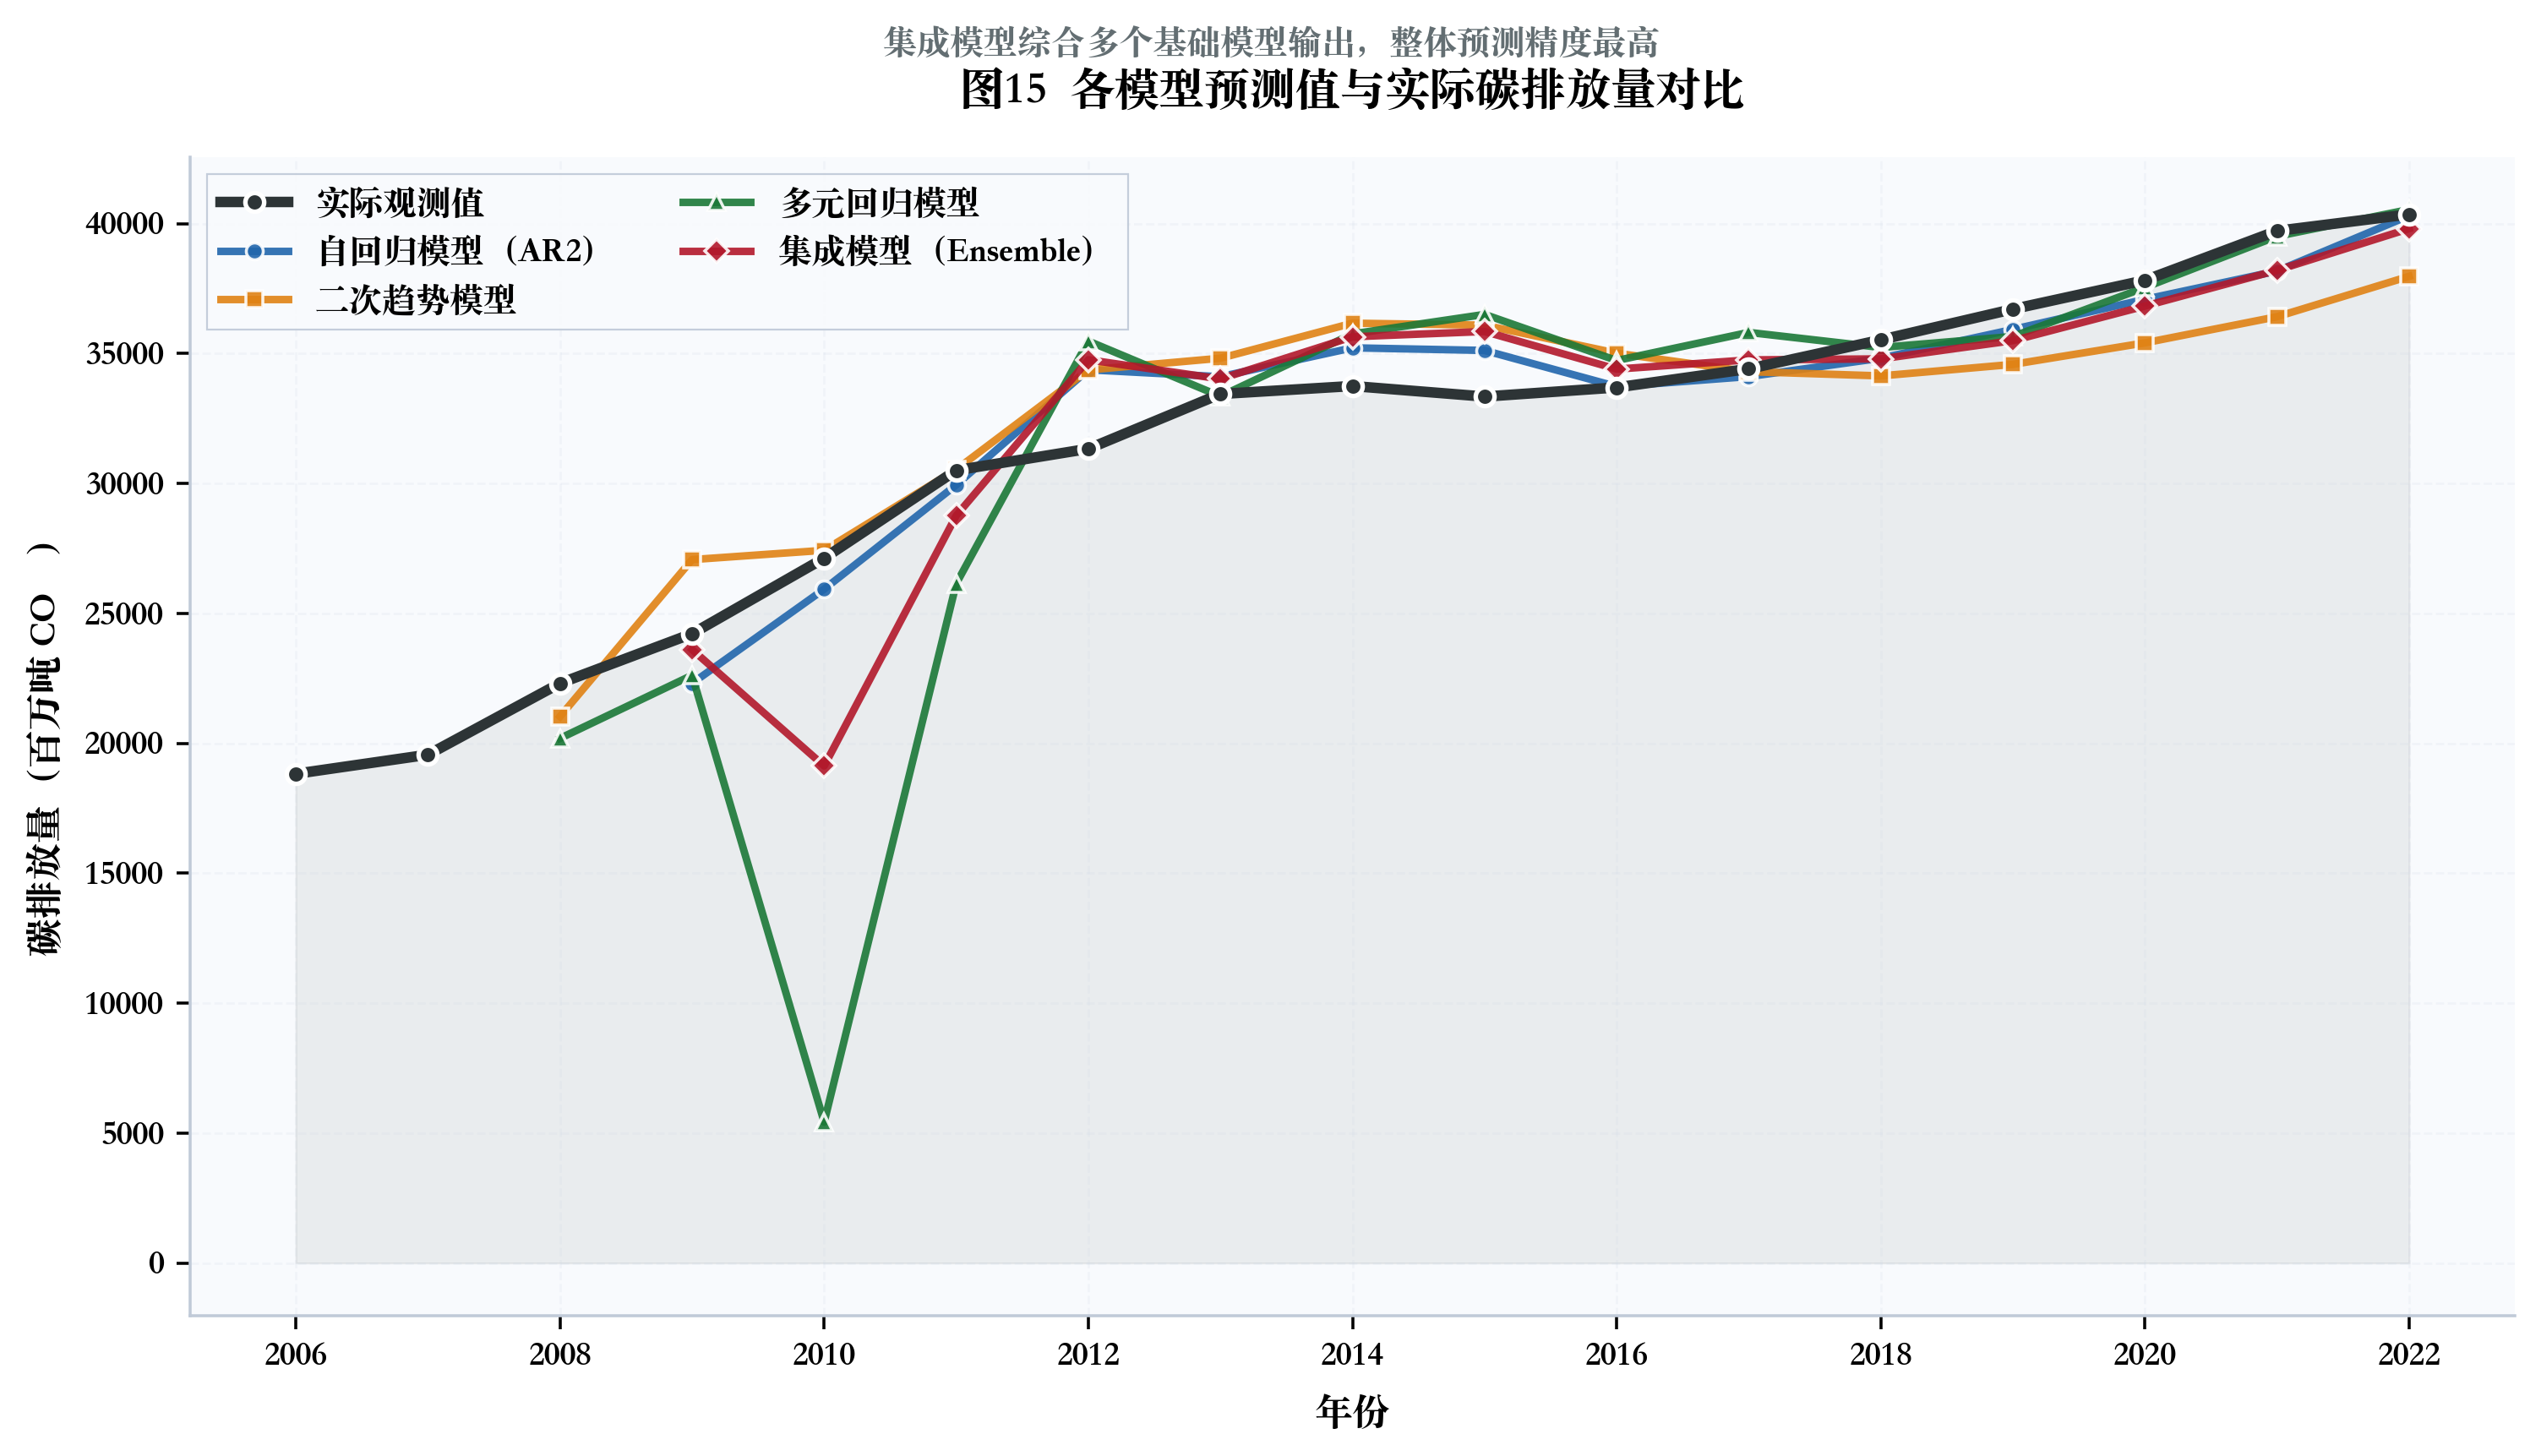
\includegraphics[width=0.82\textwidth]{../outputs/figures/Fig15_actual_vs_predicted.png}
    \caption{实际值与预测值对比图}
\end{figure}



\begin{figure}[H]
    \centering
    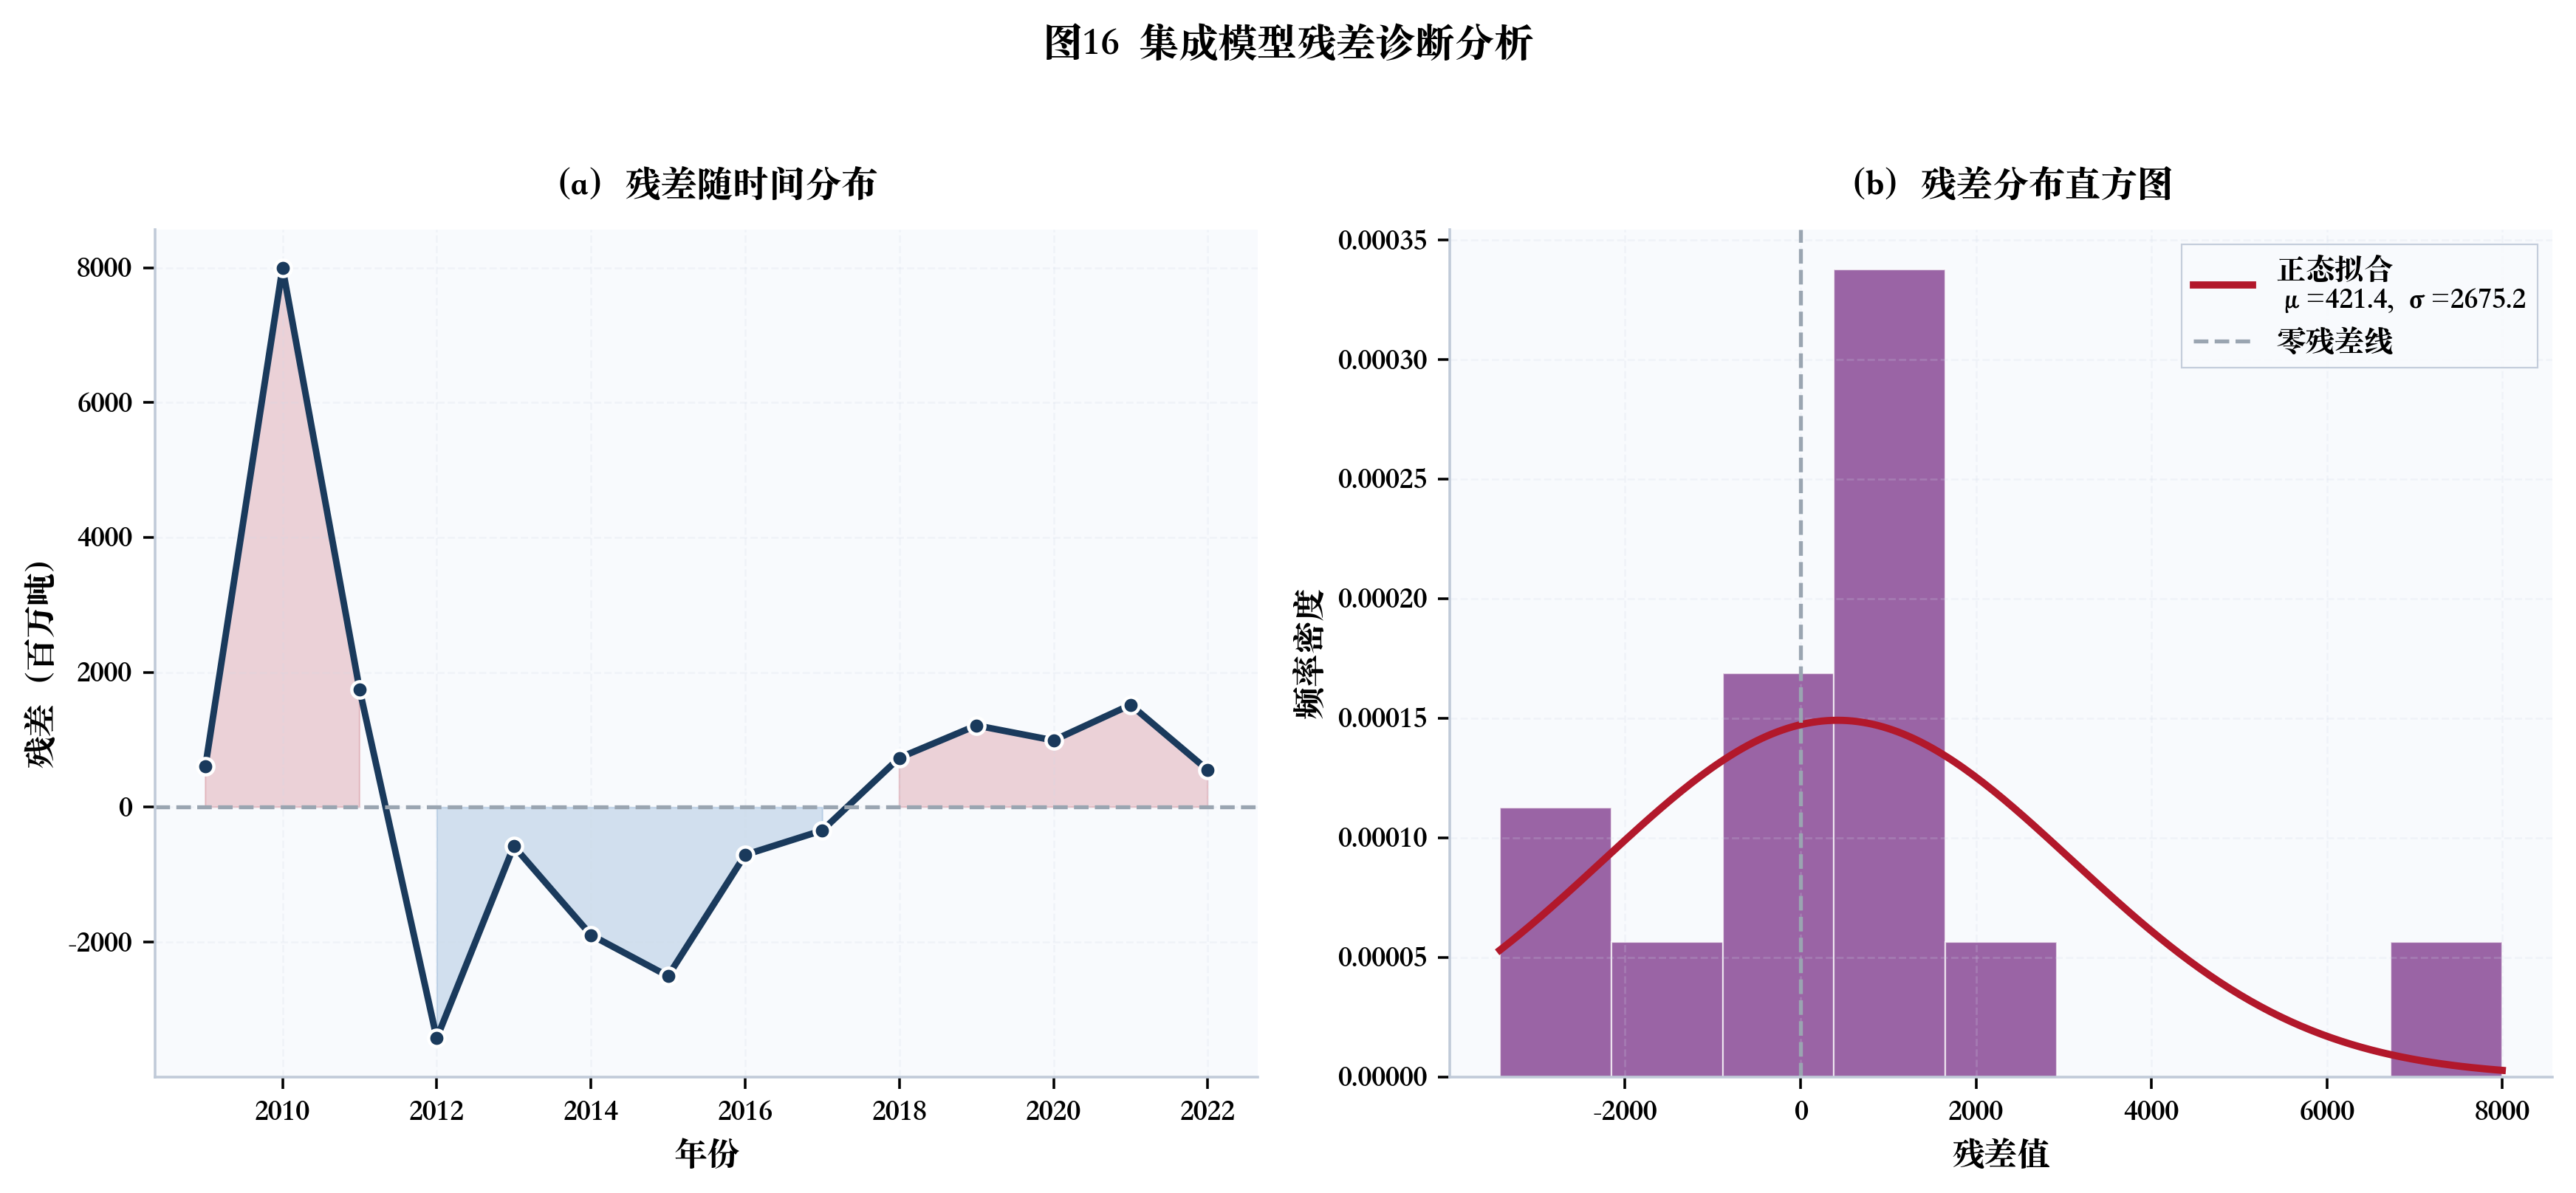
\includegraphics[width=0.92\textwidth]{../outputs/figures/Fig16_residual_diagnostics.png}
    \caption{集成模型残差诊断图}
\end{figure}



\begin{figure}[H]
    \centering
    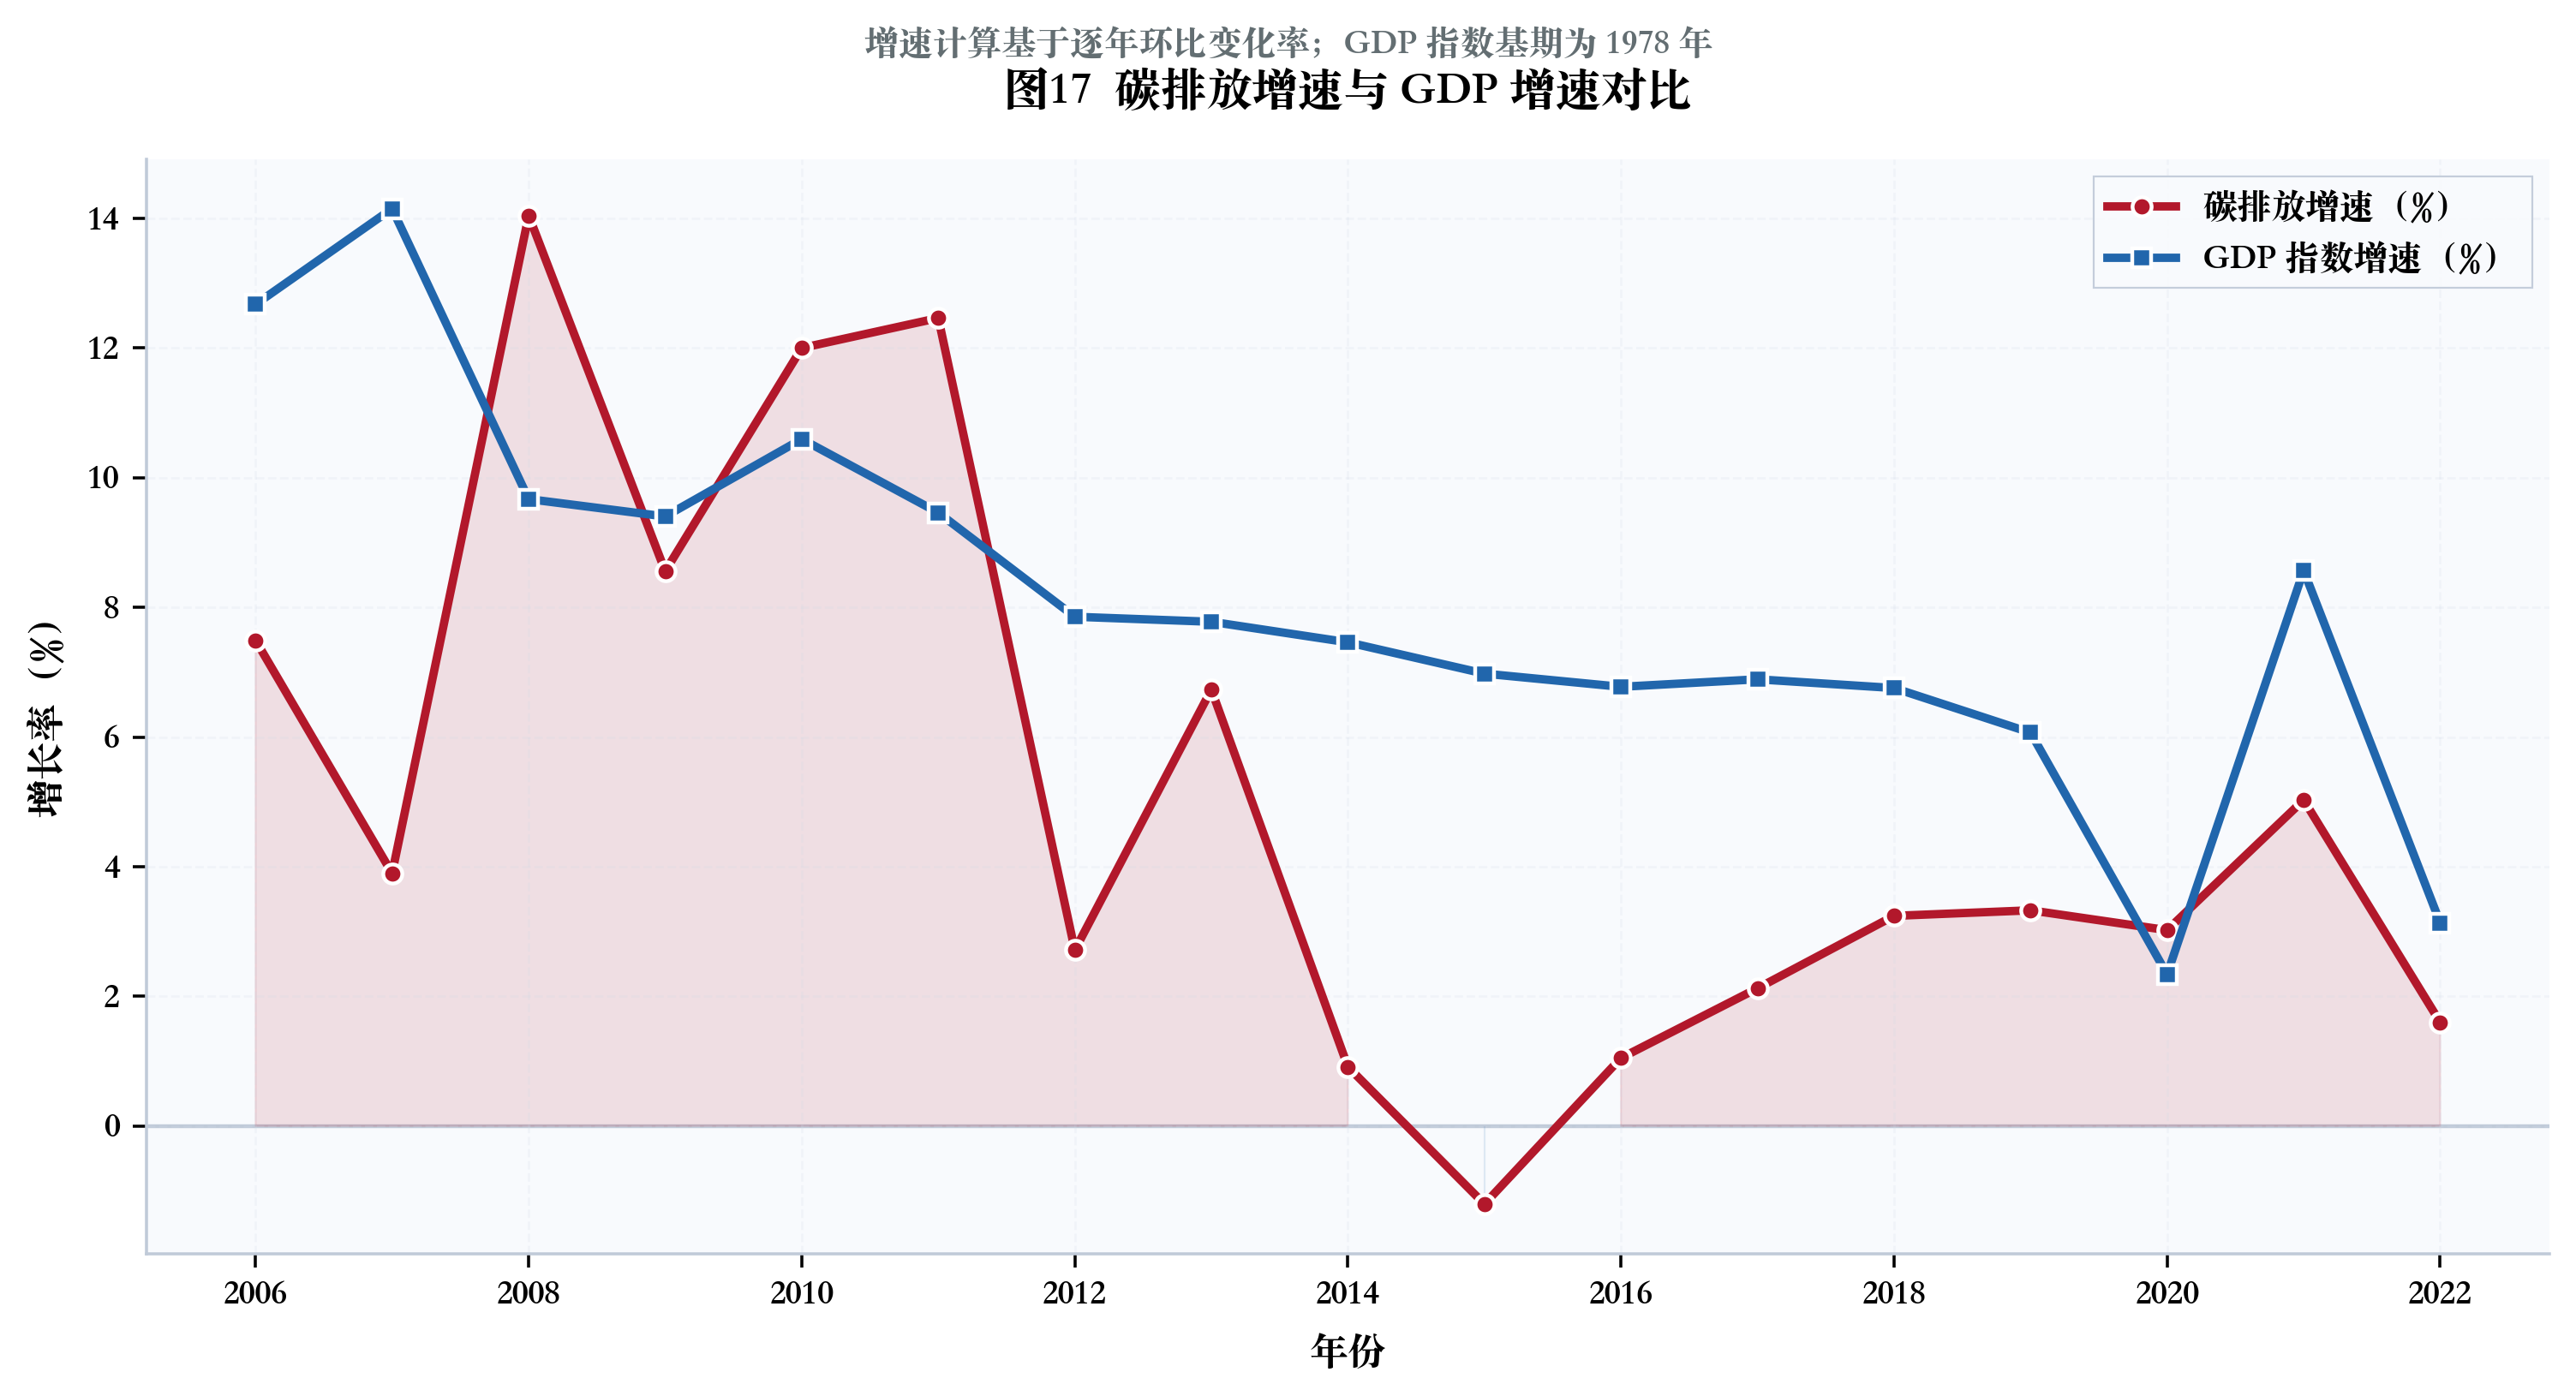
\includegraphics[width=0.82\textwidth]{../outputs/figures/Fig17_growth_rate_comparison.png}
    \caption{碳排放与GDP增速对比图}
\end{figure}



\begin{figure}[H]
    \centering
    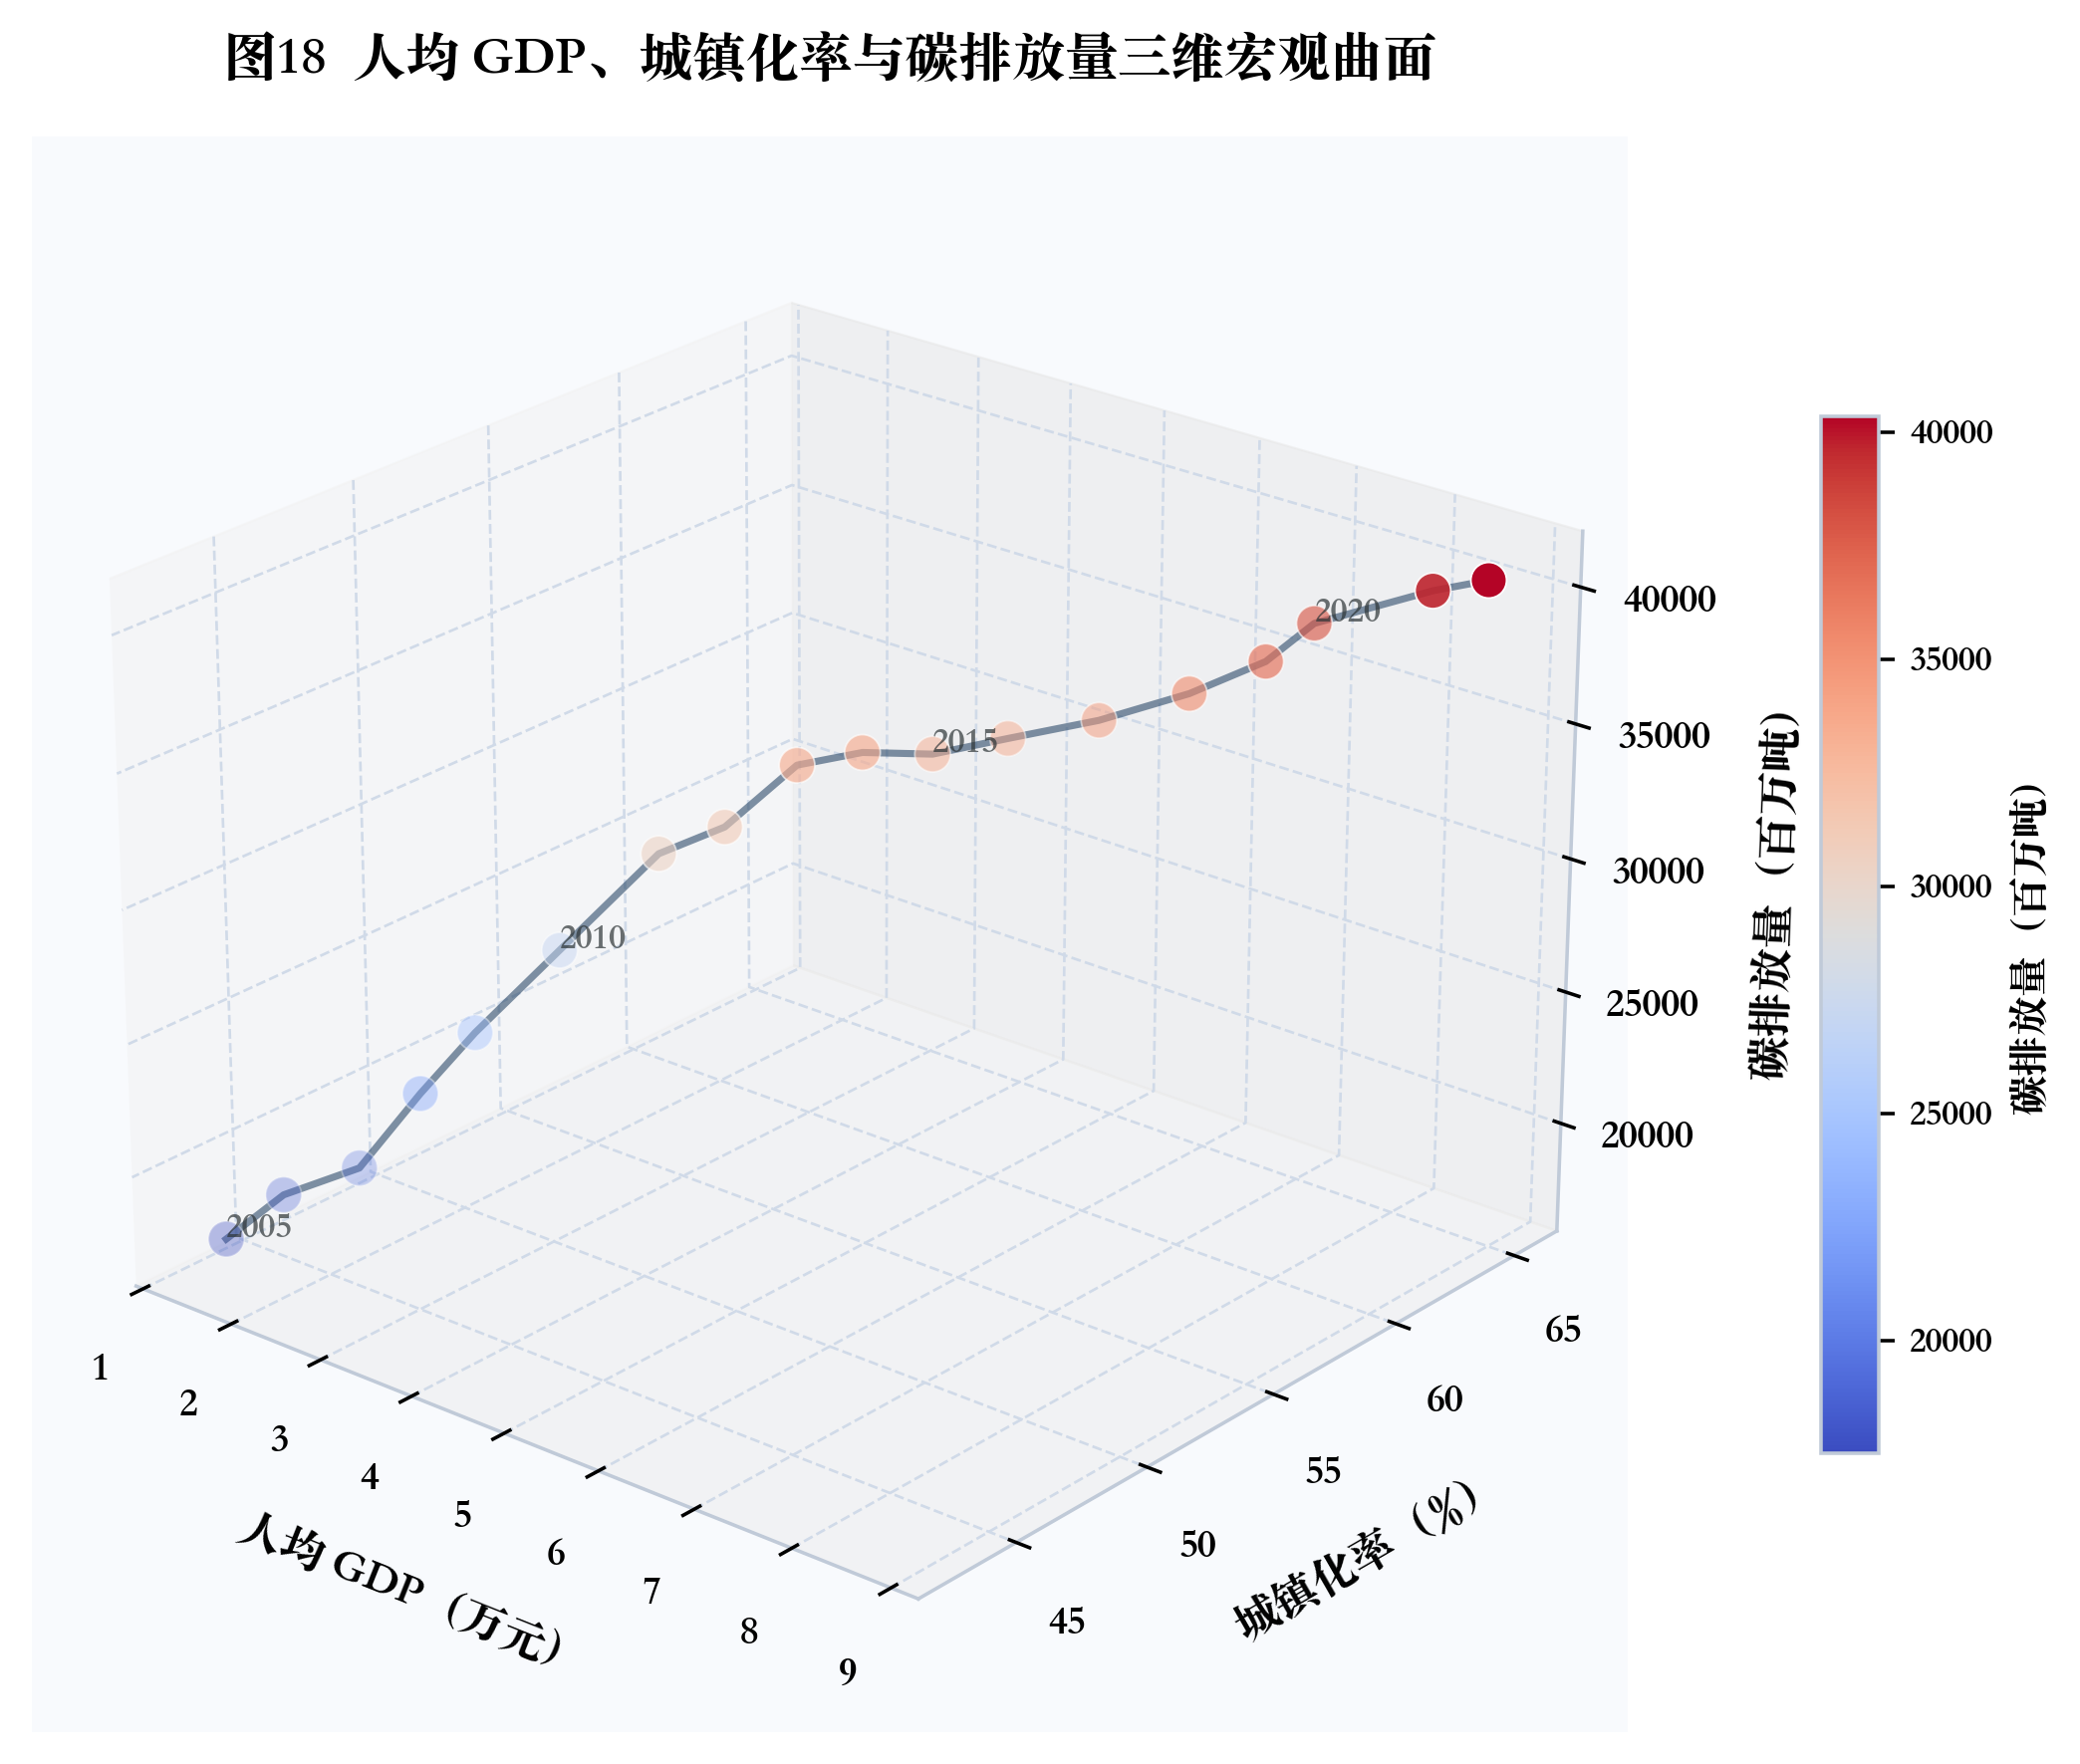
\includegraphics[width=0.78\textwidth]{../outputs/figures/Fig18_3d_macro_surface.png}
    \caption{GDP、城镇化与碳排放三维响应图}
\end{figure}



\begin{figure}[H]
    \centering
    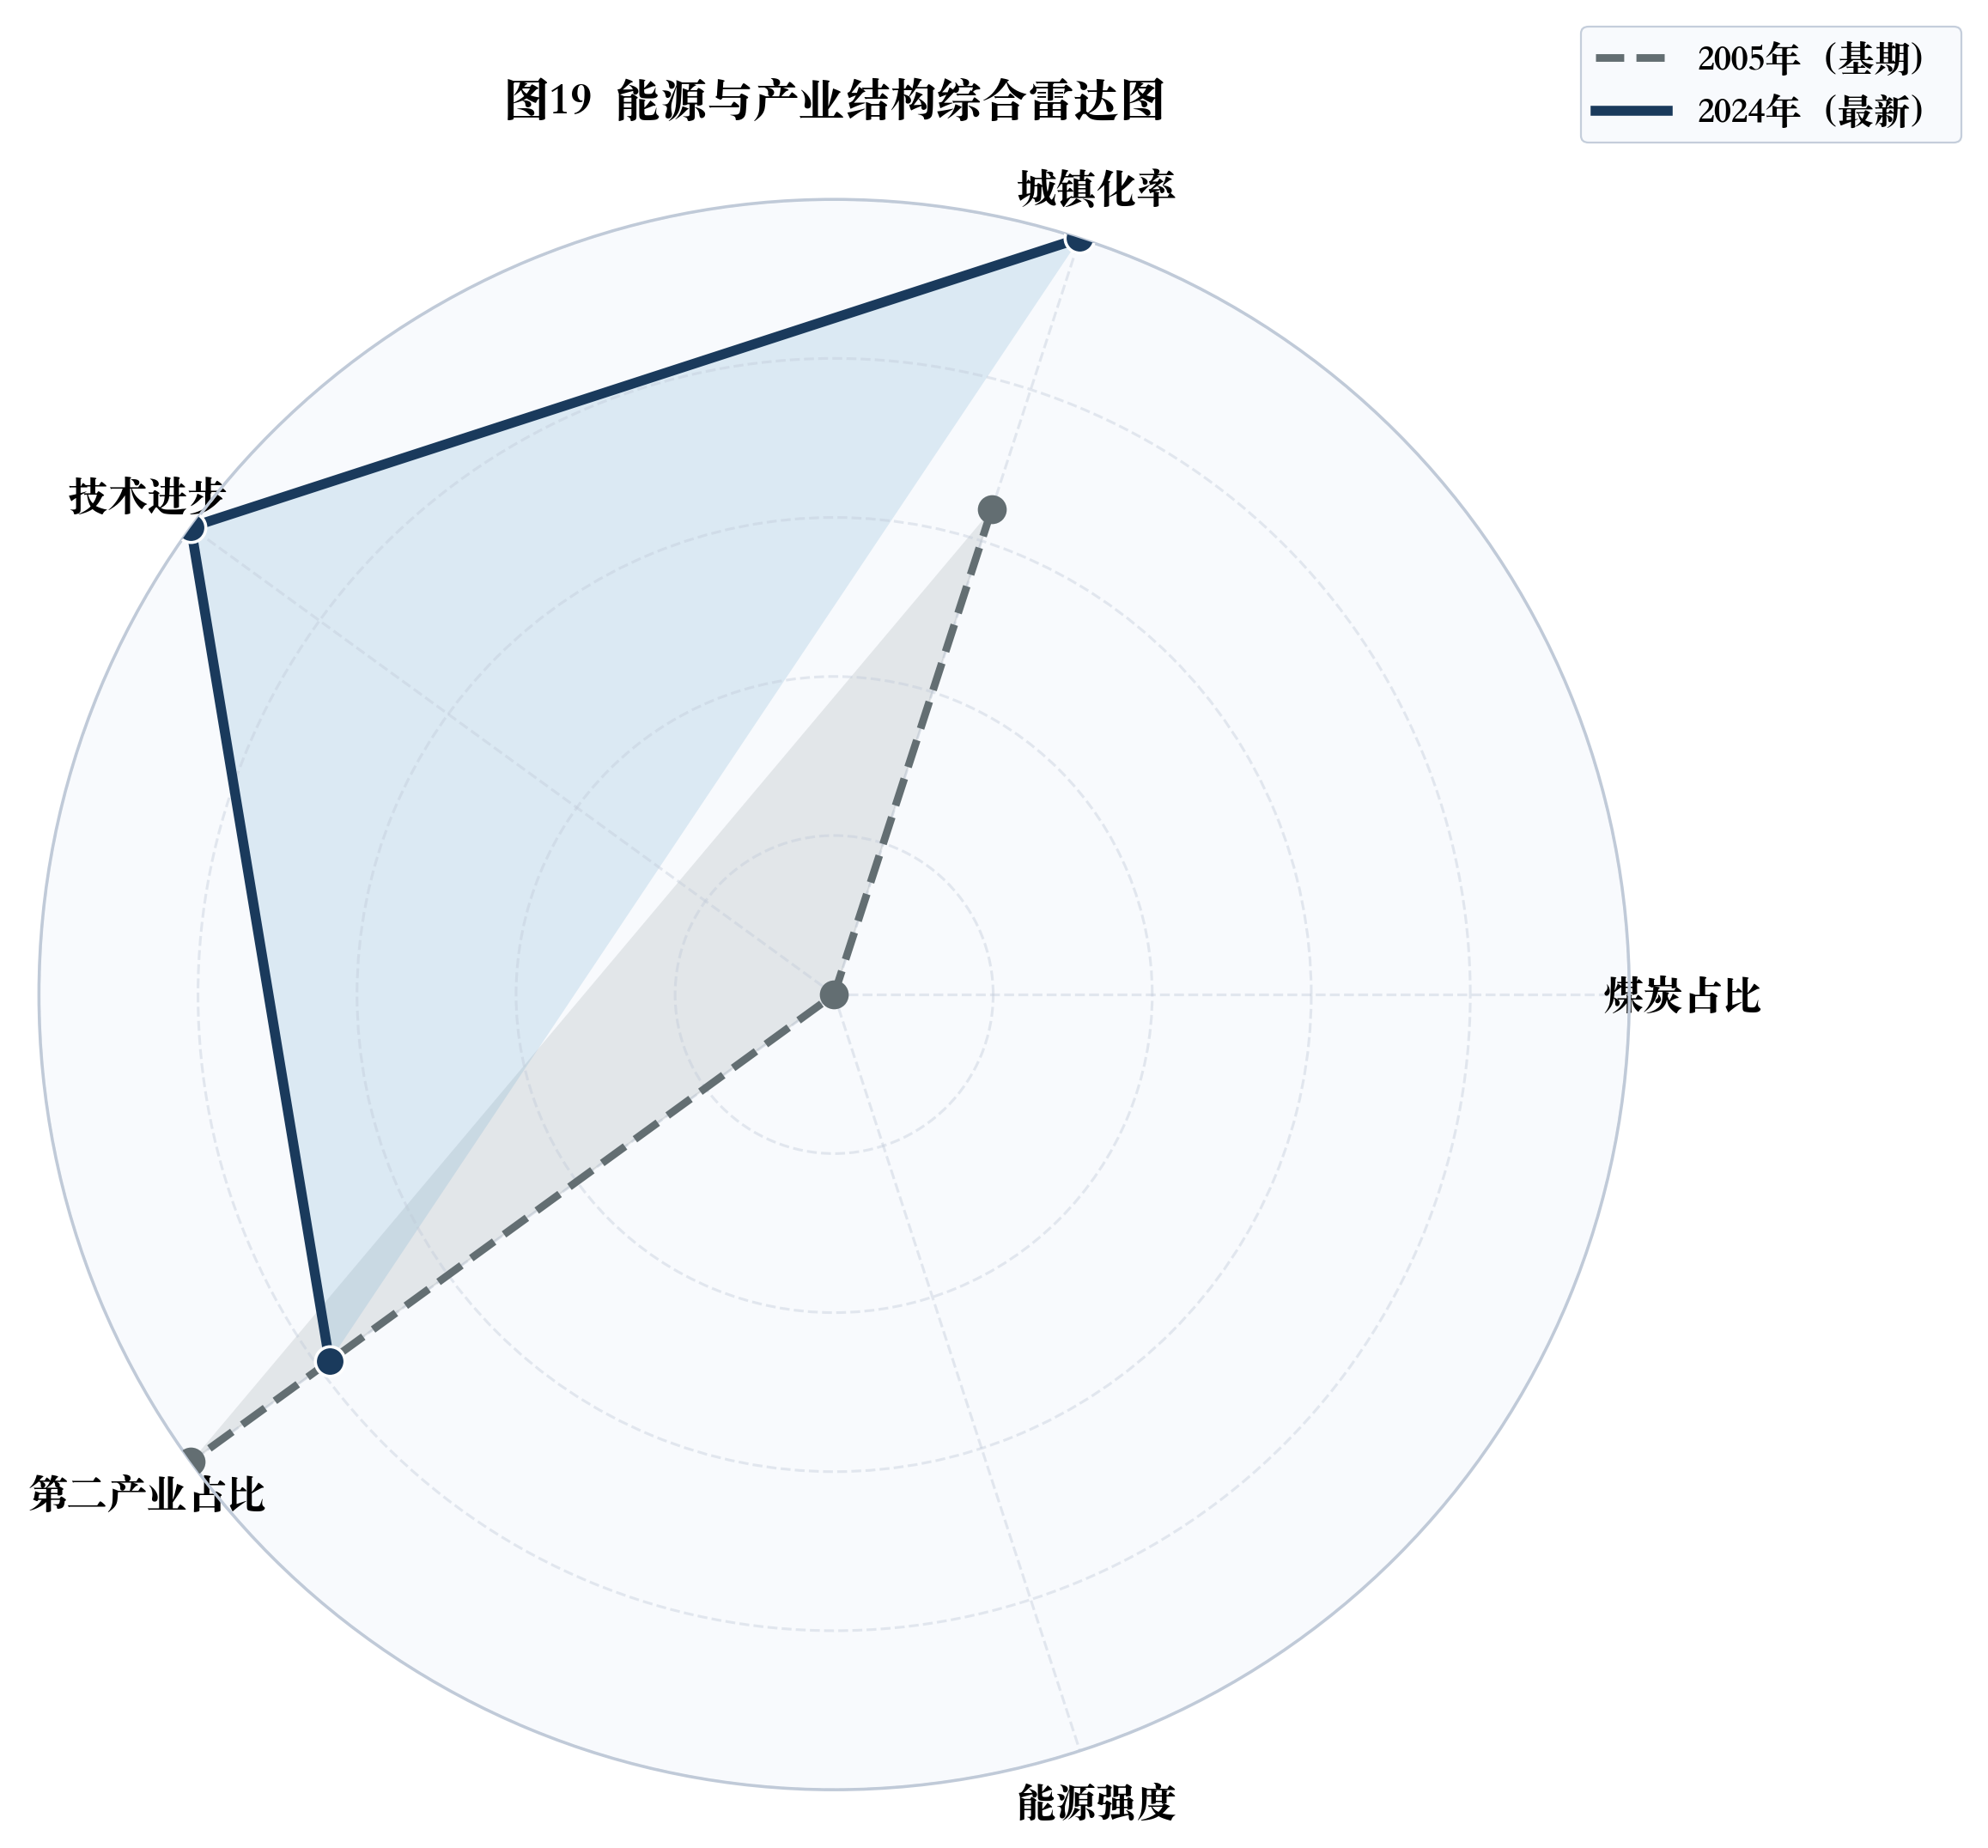
\includegraphics[width=0.62\textwidth]{../outputs/figures/Fig19_energy_radar.png}
    \caption{能源与结构特征雷达图}
\end{figure}



\begin{figure}[H]
    \centering
    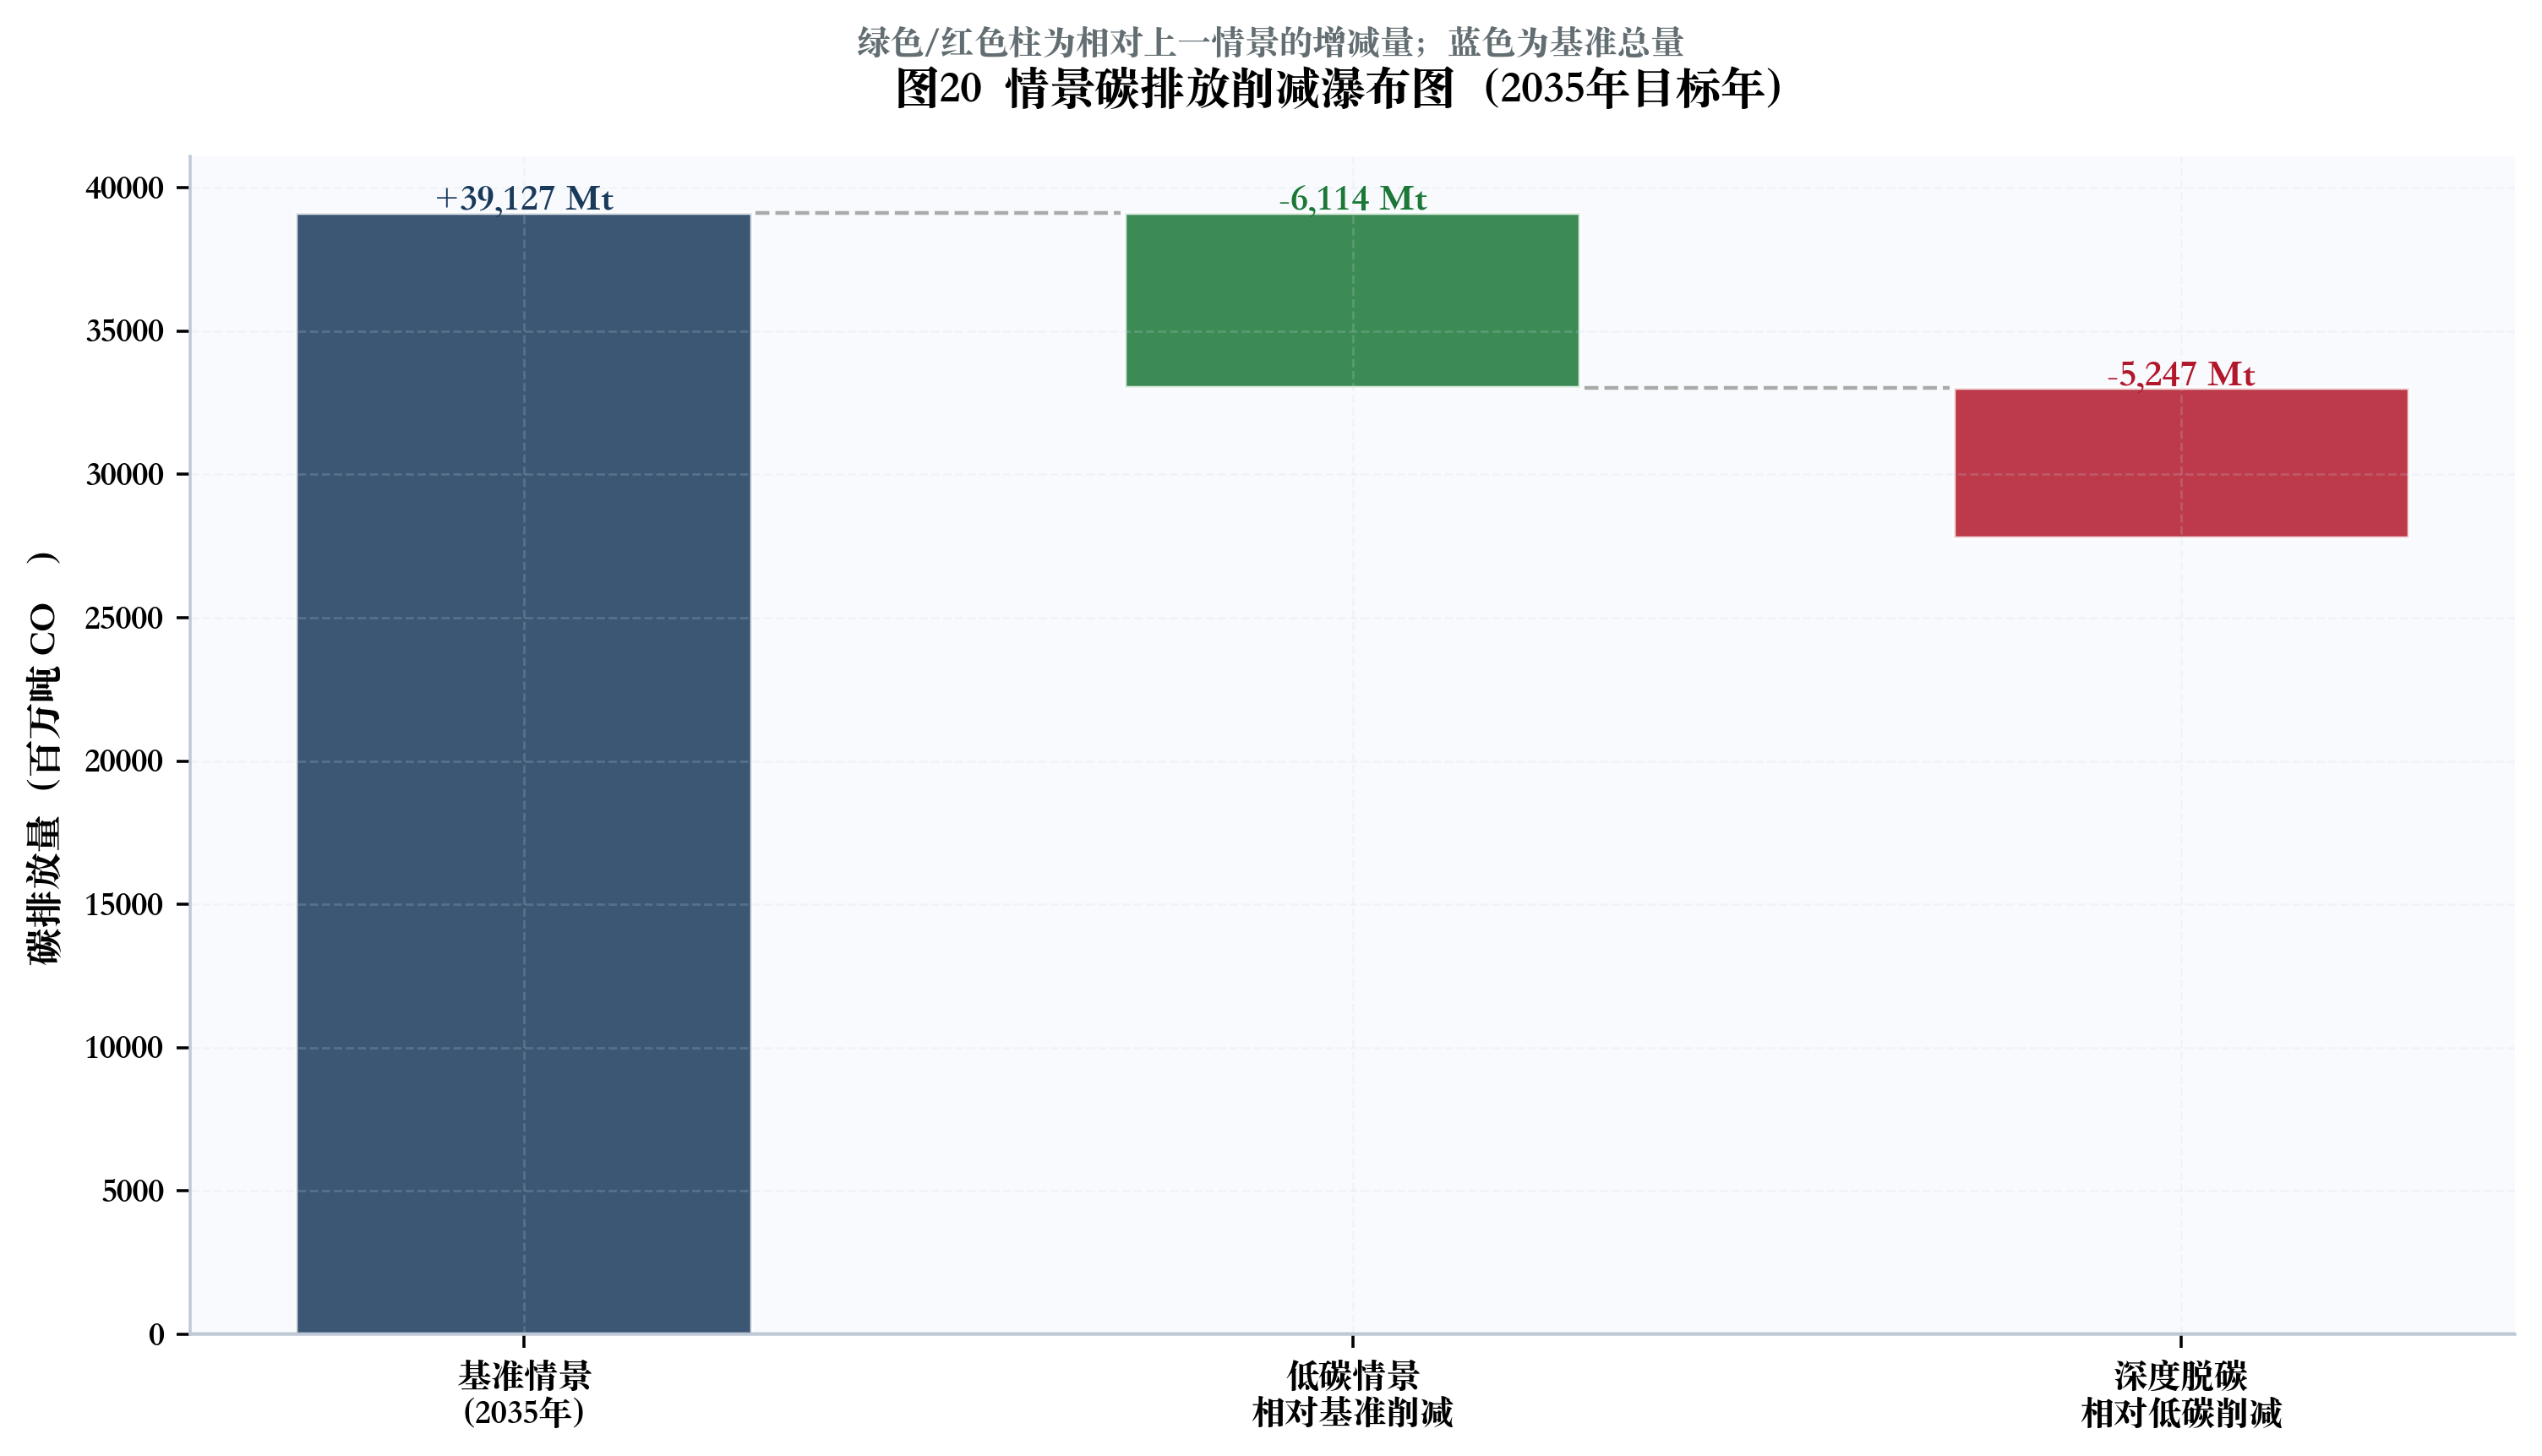
\includegraphics[width=0.82\textwidth]{../outputs/figures/Fig20_scenario_waterfall.png}
    \caption{2035年情景差异瀑布分解图}
\end{figure}



\begin{figure}[H]
    \centering
    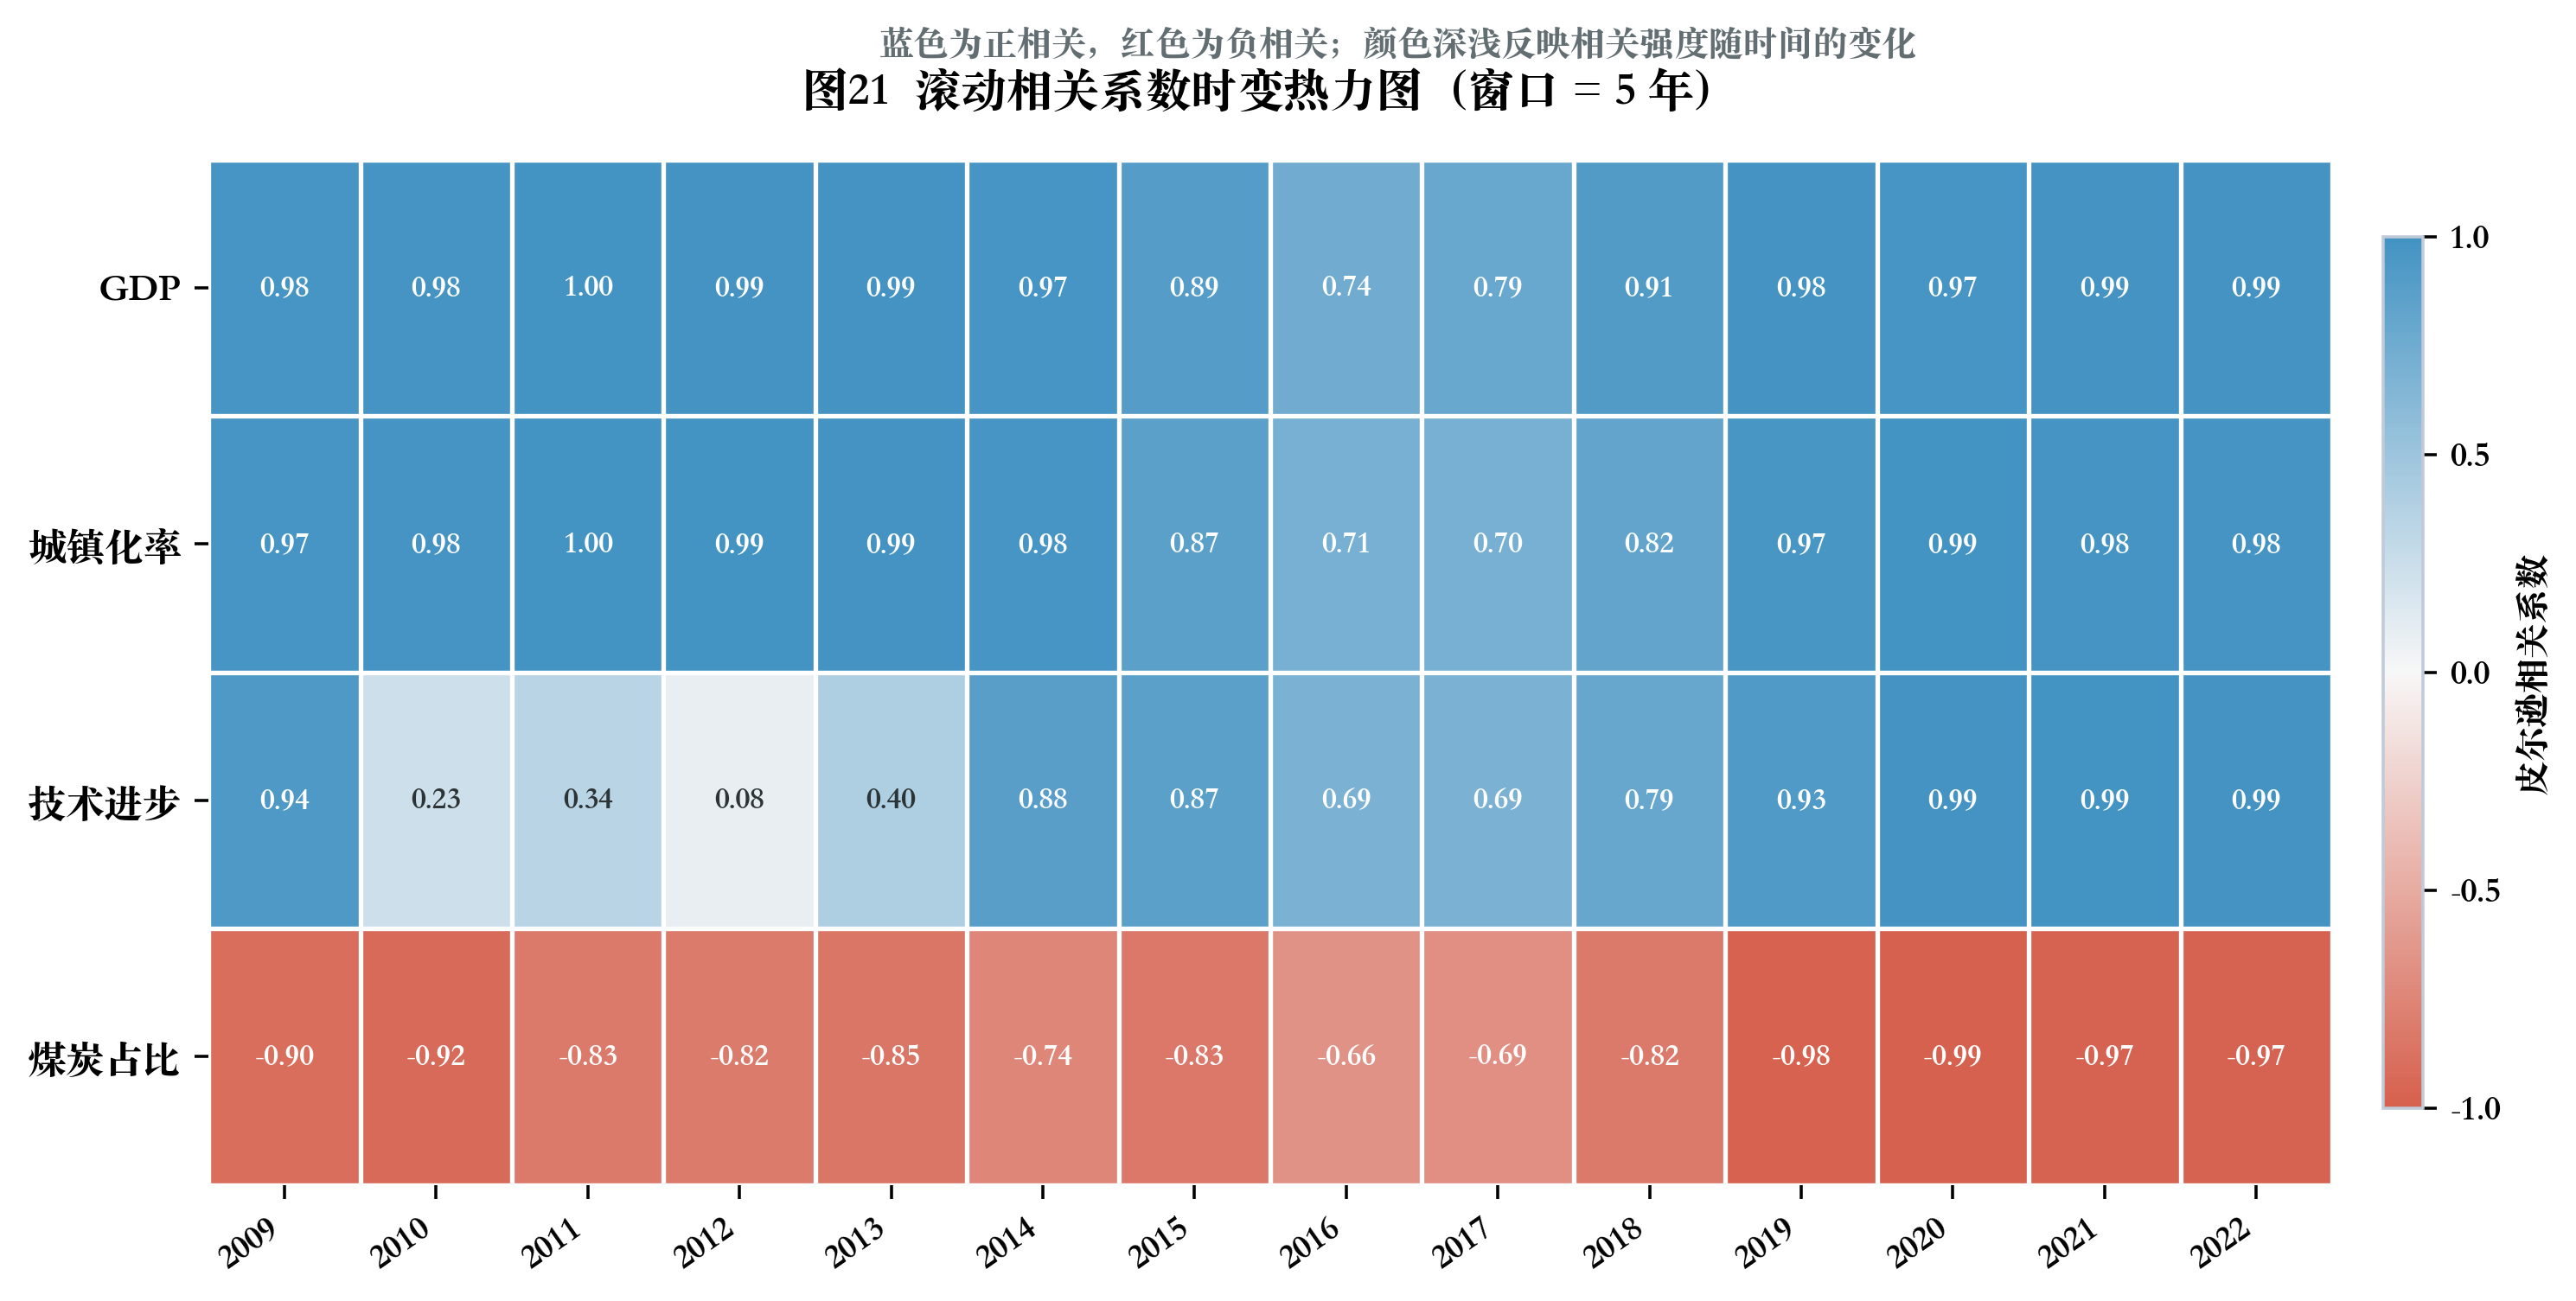
\includegraphics[width=0.88\textwidth]{../outputs/figures/Fig21_rolling_correlation_heatmap.png}
    \caption{滚动相关热力图}
\end{figure}



\subsection{附录表与补充解释}
附录表集中呈现样本描述性统计，明确变量量级与波动范围，为正文弹性系数解释与情景设定提供量纲支撑。综合附录图表，本文主结论在不同诊断视角下保持一致，附录结果视为对正文结论的稳健性补强。

\begin{table}[H]
\centering
\caption{样本描述性统计}
\begin{tabular}{ccccc}
\toprule
变量 & 均值 & 标准差 & 最小值 & 最大值 \\
\midrule
CO2 emissions & 30566.50 & 7257.68 & 17516.39 & 40358.26 \\
Population & 1368.14 & 37.21 & 1307.56 & 1412.60 \\
GDP & 654617.21 & 329391.17 & 189907.50 & 1234029.40 \\
GDP per capita & 4.73 & 2.28 & 1.45 & 8.74 \\
Urbanization & 0.55 & 0.07 & 0.43 & 0.65 \\
Secondary share & 42.24 & 3.70 & 36.90 & 46.90 \\
Coal share & 0.65 & 0.06 & 0.56 & 0.73 \\
\bottomrule
\end{tabular}
\end{table}

\subsection{附录结论性说明}
综合附录图表，本文主结论在不同可视化和诊断视角下保持一致：一是规模效应仍然存在，但结构优化已开始改变增长轨迹；二是模型外推能力受样本规模约束明显，稳健性优先于复杂度；三是政策路径差异主要体现在峰值平台和下降斜率，而非单一年份变化。附录结果因此可视为对正文结论的稳健性补强，而非替代性结论。



\end{document}
